\section{Results for $\pi, K, p$} 
In this section
, we show the results of $v_{1}$ and $v_{2}$ for pions, kaons, and proton. The $p_{T}$ and rapidity dependence will be discussed and performed in three centrality classes 0-10\%, 10-40\% and 40-60\%. These results will be comparison to STAR BES-I results and the physics meaning will be discussed.

\subsection{$v_{1}$ results for $\pi, K, p$}
In this chapter, we will show the $v_{1}$ as a function of $p_{T}$ and rapidity(y) in fine centrality bins for $\pi^{\pm}, K^{\pm}$ and proton. In the $v_{1}$  vs. rapidity distribution, in order to quantify the strength of  $v_{1}$, we will fit the $v_{1}$ vs. y distribution with this equation \ref{fit_v1_formula}. As can see, pion's $v_{1}$ is positive in the central collision while is negative in the mid-central and peripheral collision.

\begin{equation} \label{fit_v1_formula}
	v_{1}(y) = F*y + C*y^{3} +b 
\end{equation}
Where parameter F is the $v_{1}$ slop $dv_{1}/dy$, parameter C is the fluctuation term and parameter b is the offset to origin point.

\subsubsection{pions $v_{1}$ as a function of $p_{T}$ and rapidity}
Figure \ref{pion_v1y_cent} shows $\pi^{+}, \pi^{-}$ $v_{1}$ as a function of y for different centrality bins from 0-5\% to 50-60\%,  the red line is fitting function \ref{fit_v1_formula}, the $p_{T}$ range is [0.2, 1.6] GeV/c, which is same with STAR BES-I results. We also write down the fitted results $v_{1}$ slope $dv_{1}/dy$. As we can see, the magnitude of pions' $v_{1}$ has centrality dependence, figure \ref{pion_dv1dy_cent} shows $\pi^{+}, \pi^{-}$ $dv_{1}/dy$ as a function of centrality, we can clear see that the $v_{1}$ sign change from central to peripheral collision. This can be explained by the shadowing effect from spectators, because at 3 GeV, the passage time is comparable or larger than medium expansion time. So, the spectators will shadow the expansion of mediums, which will cause negative $v_{1}$ value, and this effect larger with collisions from central collision to peripheral collision.

Since STAR's BES-I directed flow results focus on the intermediate centrality interval 10-40\%. In this analysis, we also have $v_{1}$ results in such centrality bins for these particle species, and, we will calculate the energy dependence for all particles' $v_{1}$. Figure \ref{pion_v1y_widecent} shows $\pi^{+}$ and $\pi^{-}$ $v_{1}$ as a function of y in 0-10\%, 10-40\% and 40-60\% bins. We can see in the 0-10\%, the pions' $v_{1}$ is positive, and the the pions' $v_{1}$ is negative in the 10-40\% and 40-60\% centrality, which can be explained by the spectator shadowing effect.

\begin{figure}[h]
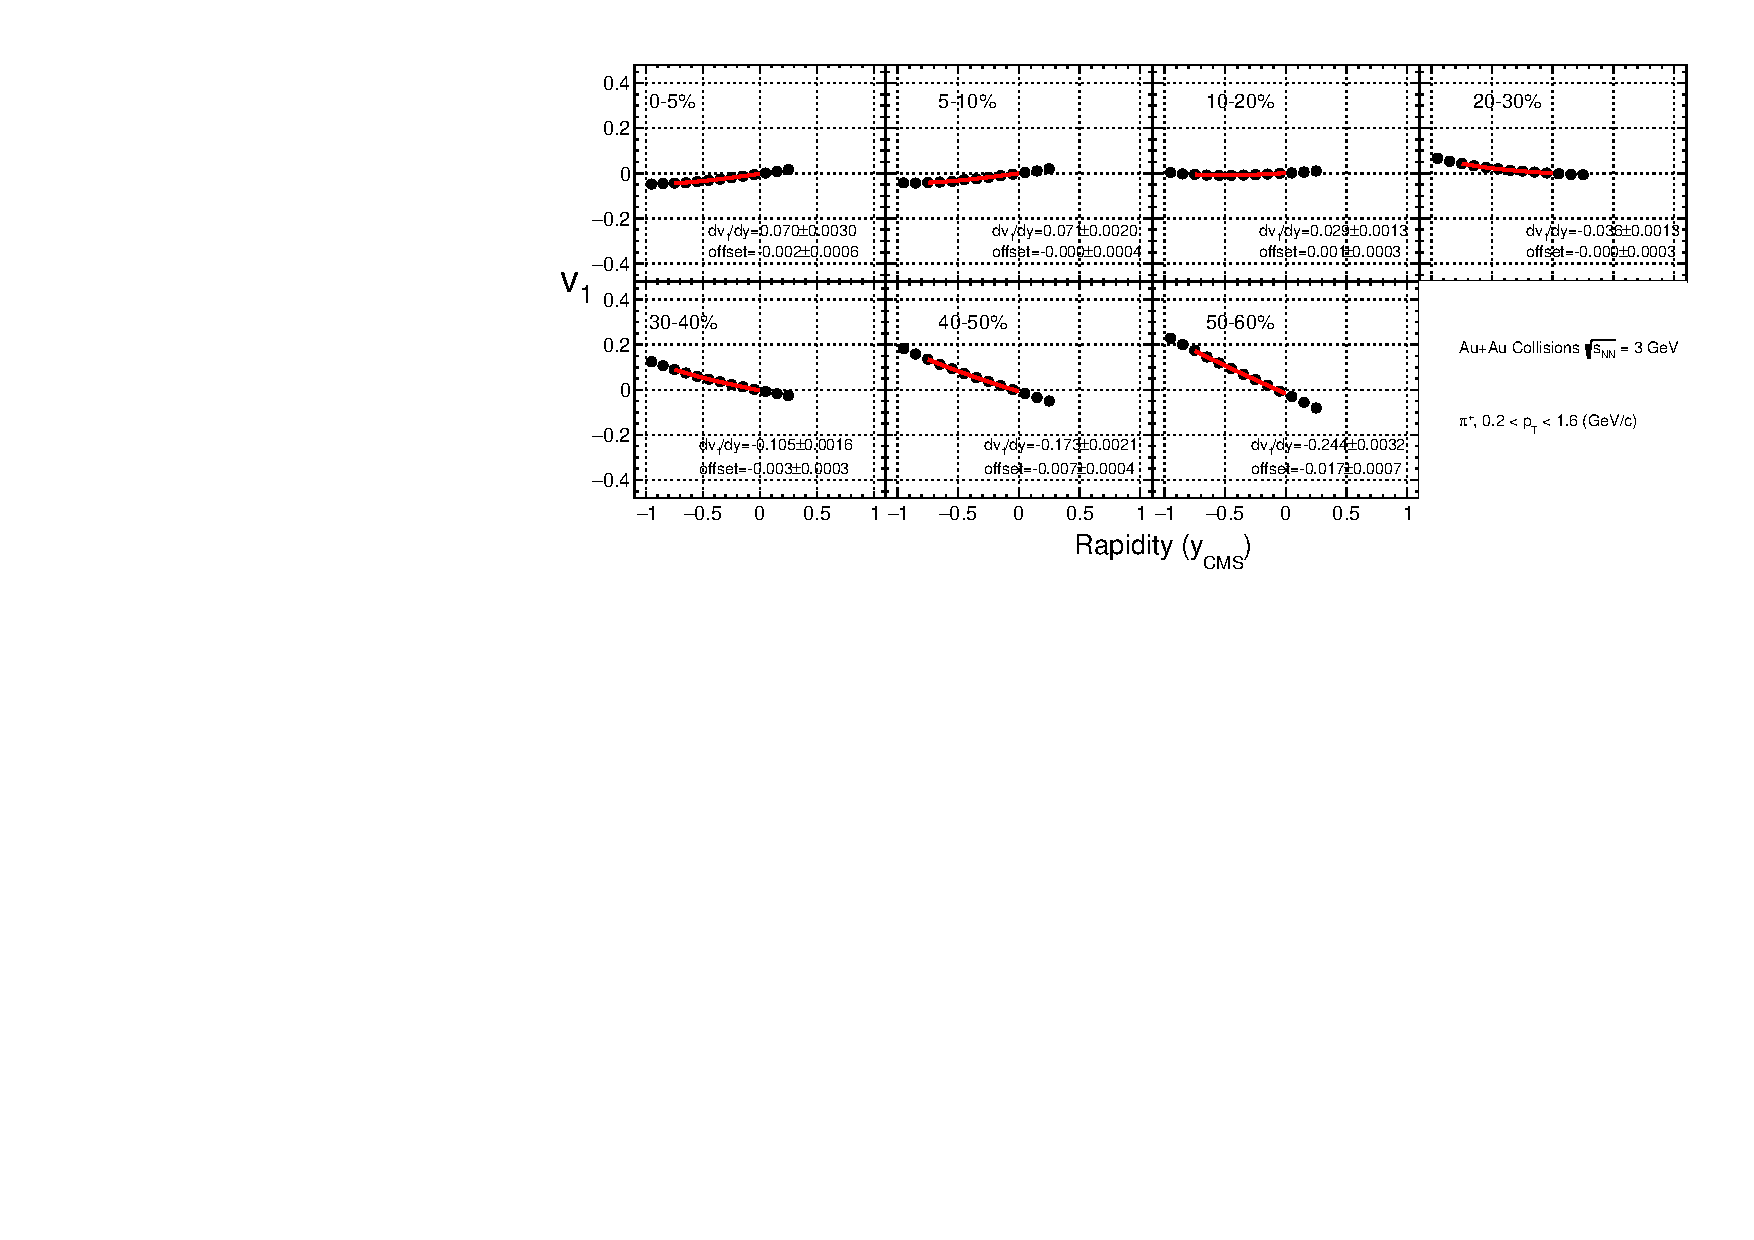
\includegraphics[scale=0.6]{chapter3/fig/v1ypikp/v1pionp_cent.pdf}
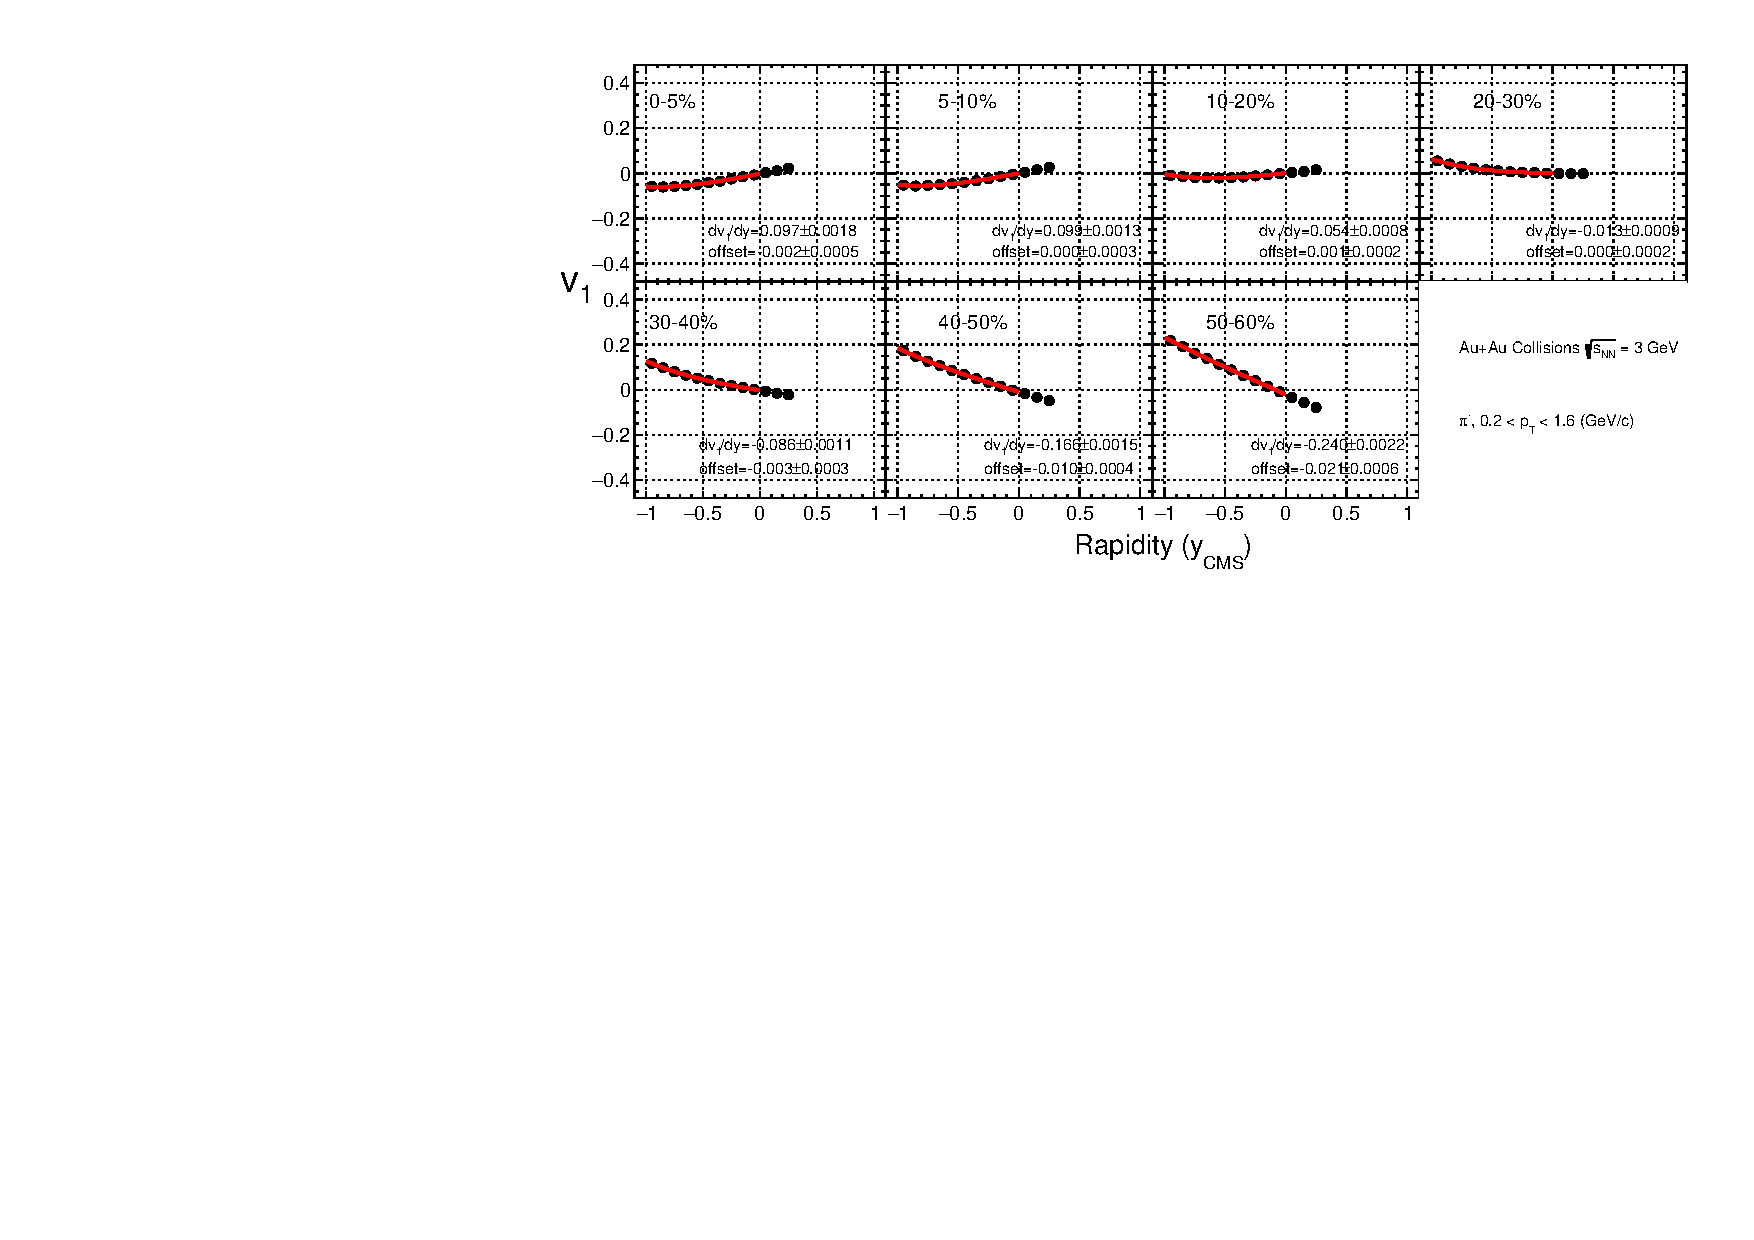
\includegraphics[scale=0.6]{chapter3/fig/v1ypikp/v1pionm_cent.pdf}
\caption{\label{pion_v1y_cent} $v_{1}$ as a function of rapidity(y) in different centrality bins for $\pi^{+}$ and $\pi^{-}$ in Au+Au collisions at $\sqrt{s_{NN}}$. The red line is fitting function.}
\end{figure}

\begin{figure}[h]
\centering
\subfigure{   
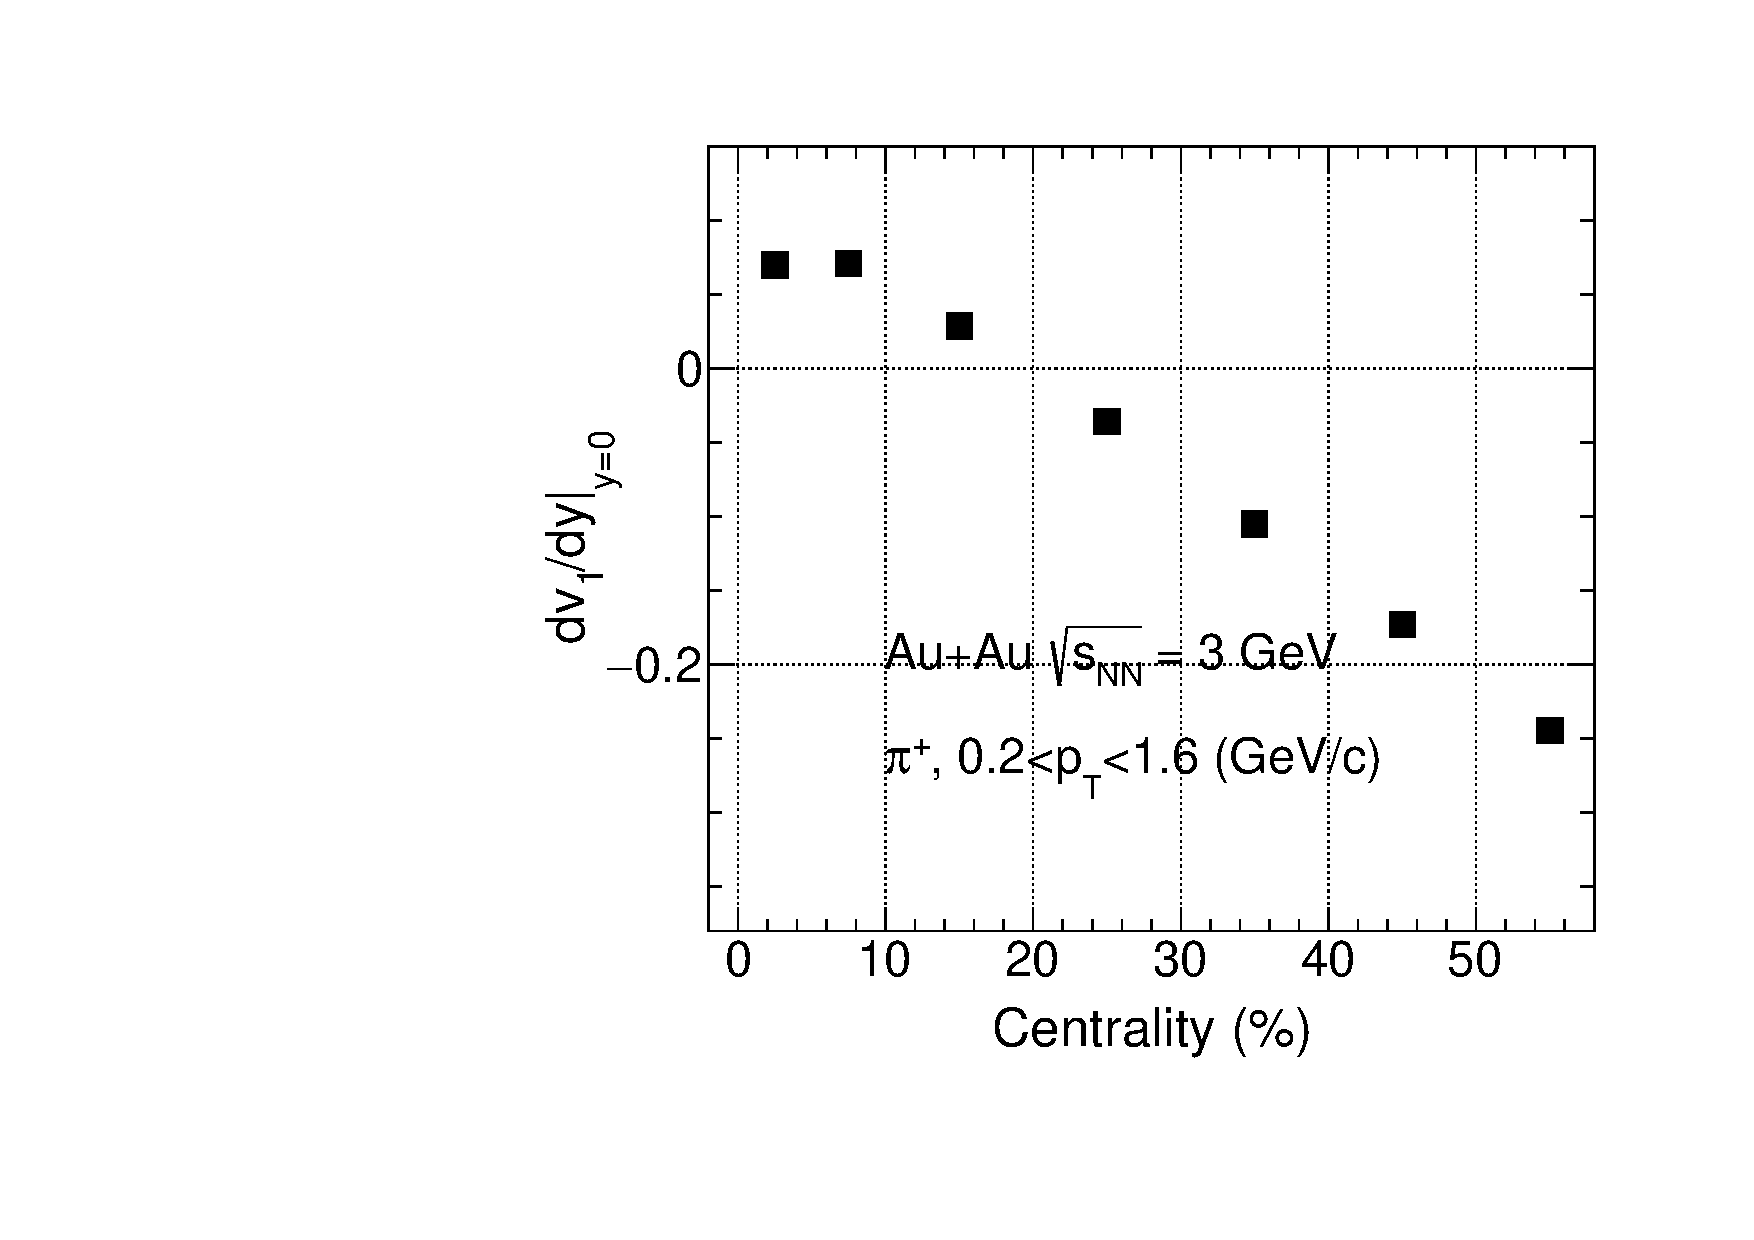
\includegraphics[width=0.45\textwidth]{chapter3/fig/v1ypikp/dv1dy_pionp.pdf}}
\subfigure{
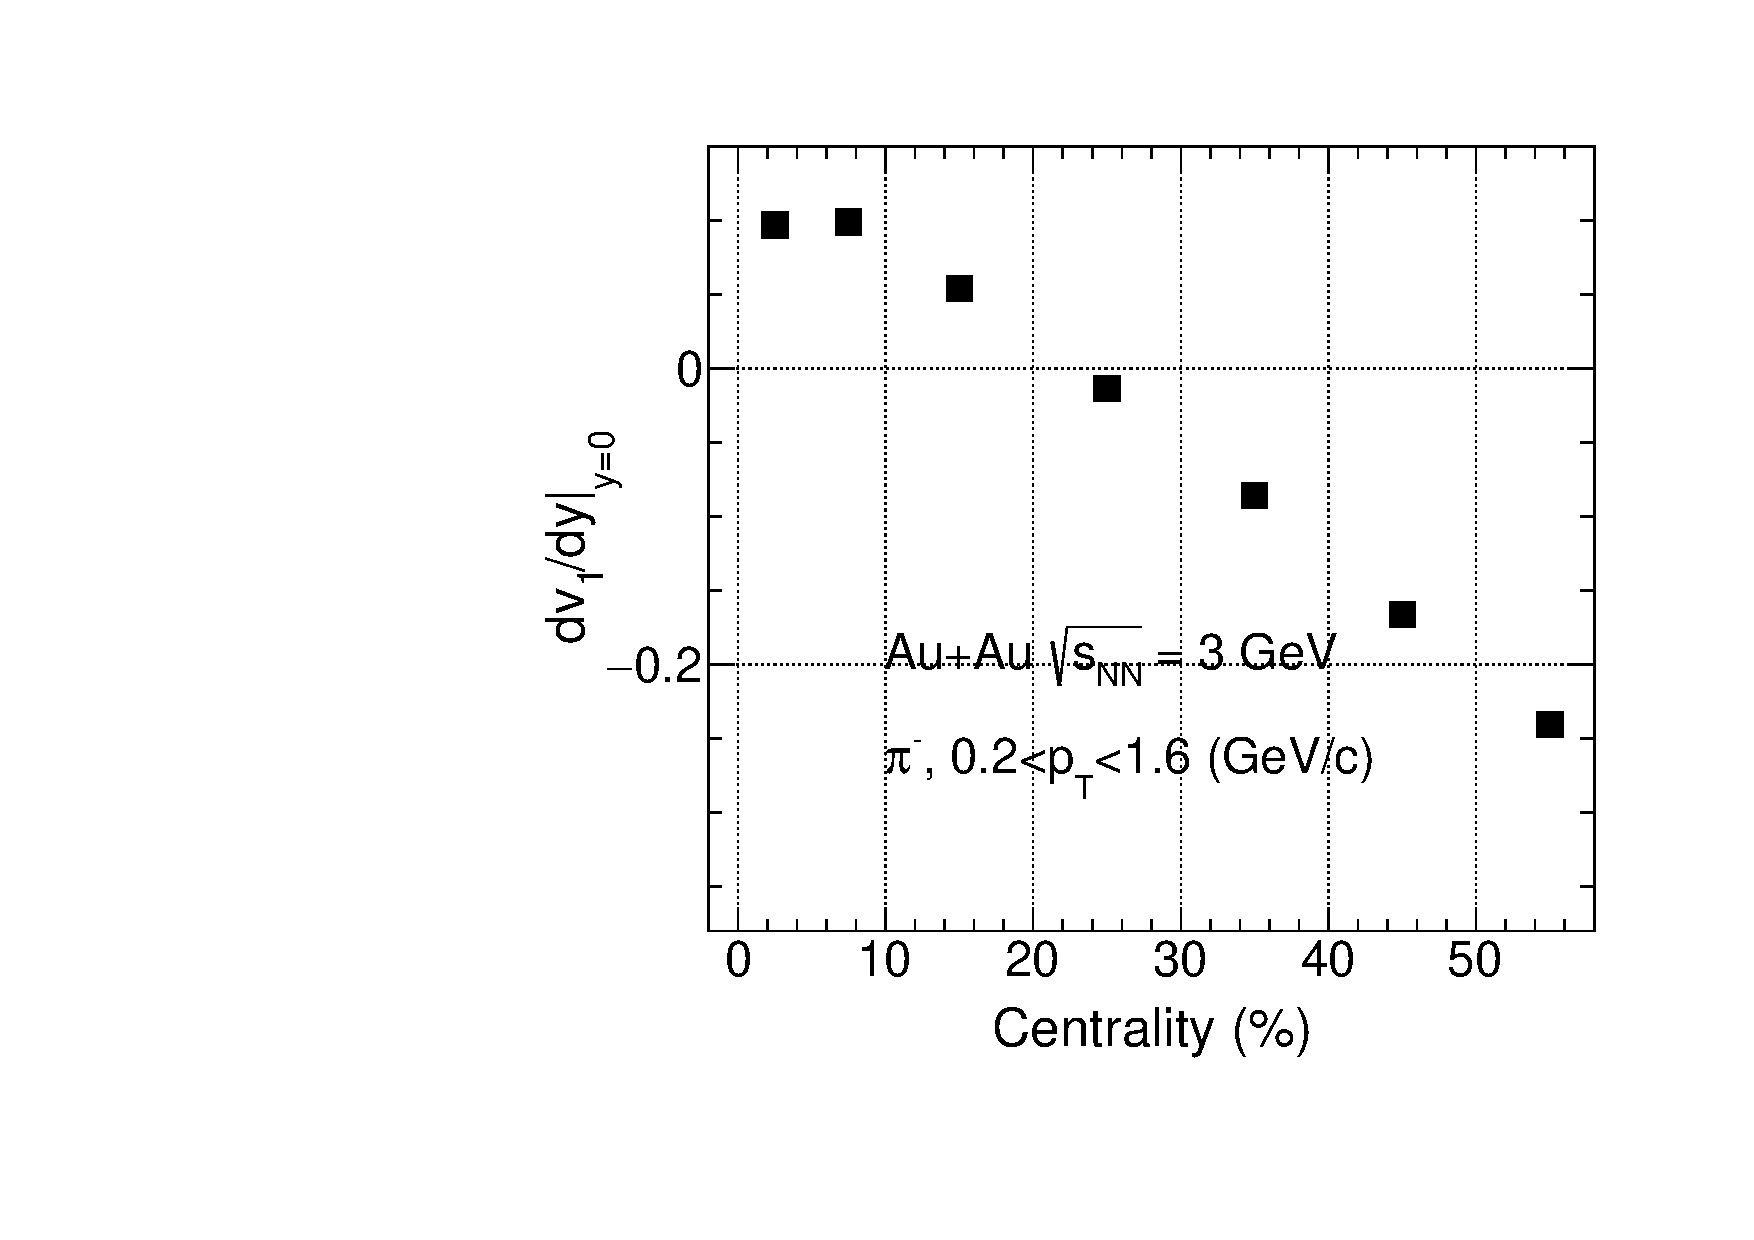
\includegraphics[width=0.45\textwidth]{chapter3/fig/v1ypikp/dv1dy_pionm.pdf}}
\caption{\label{pion_dv1dy_cent} pions' $v_{1}$ slope $dv_{1}/dy$ as a function of centrality, (left) $\pi^{+}$ (right) $\pi^{-}$ in Au+Au collisions $\sqrt{s_{NN}}$ = 3GeV.}
\end{figure}

\begin{figure}[h]
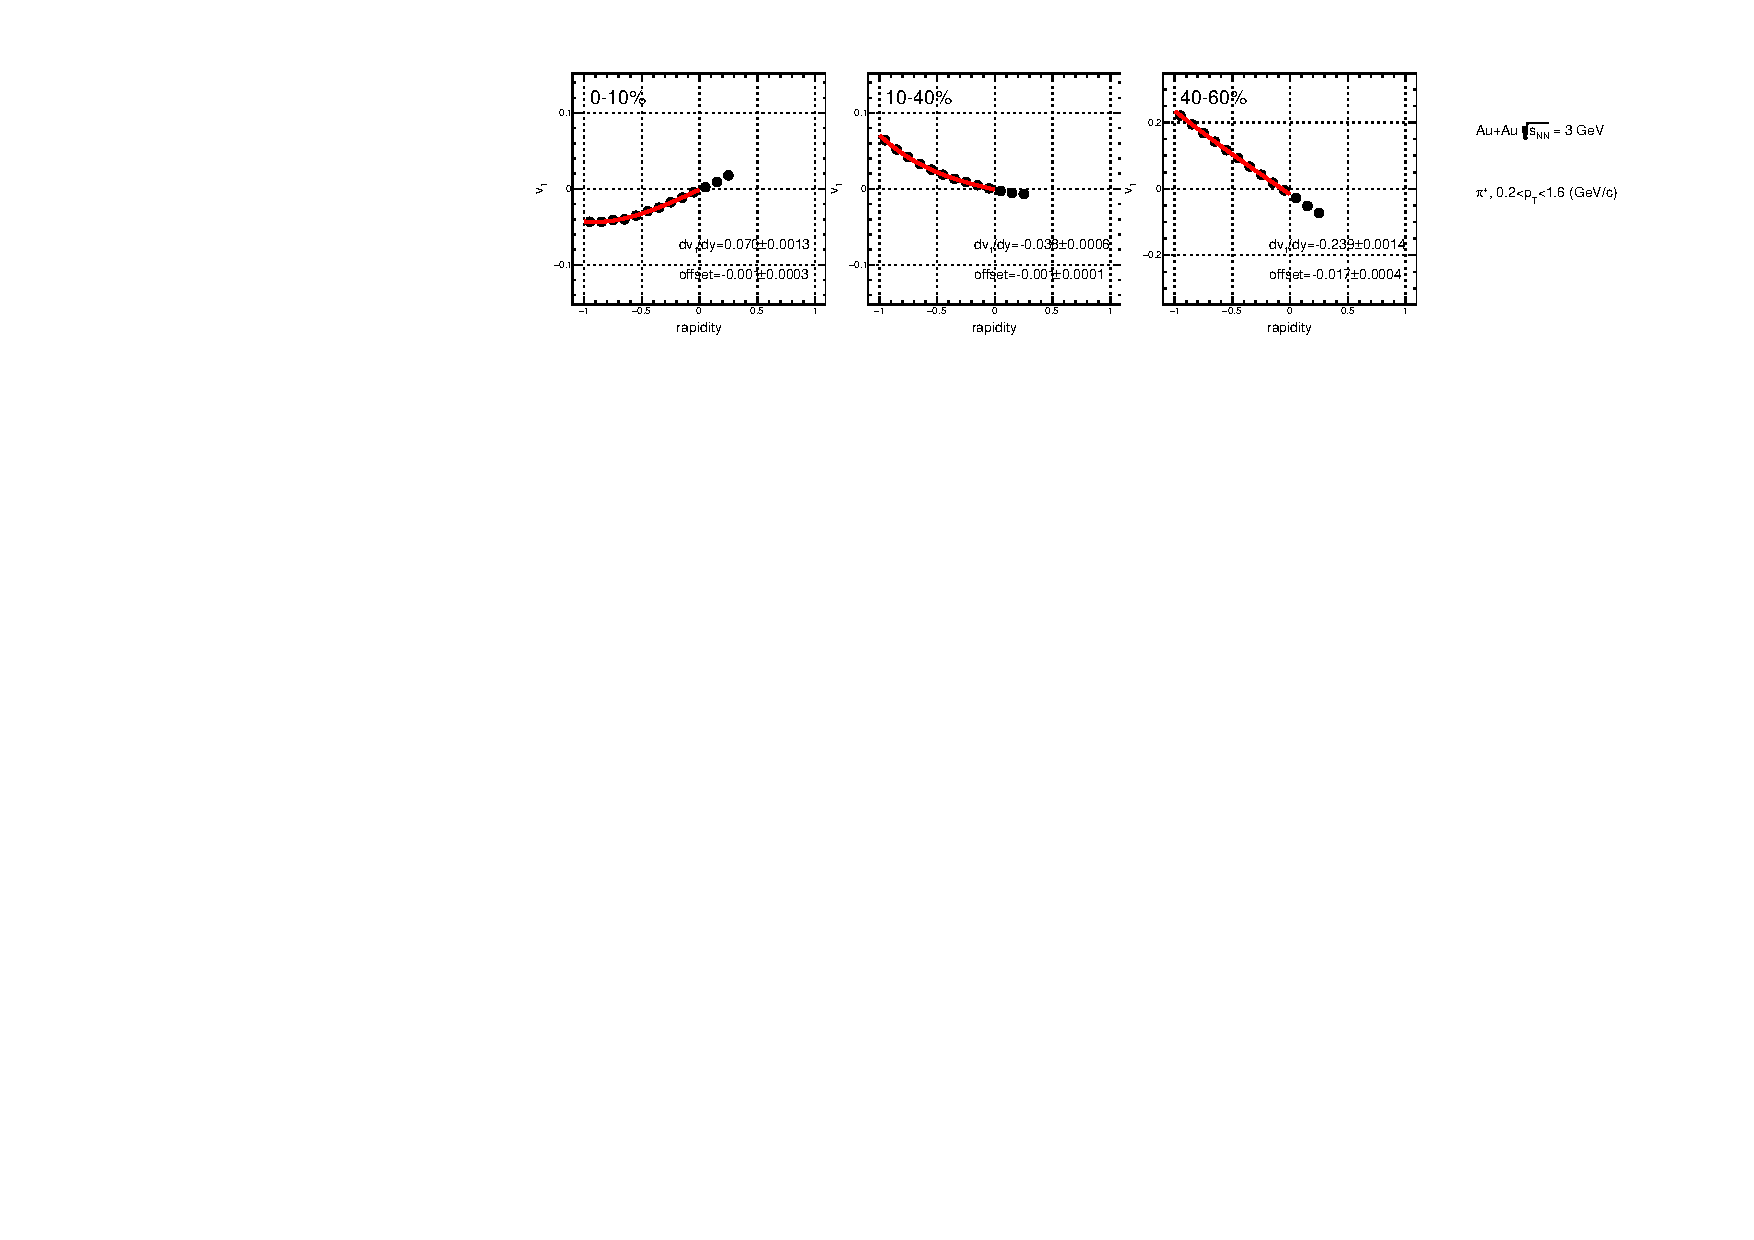
\includegraphics[scale=0.8]{FXT3gev/chapter3/fig/v1ypikp/pionp_v1y_wide_cent.pdf}
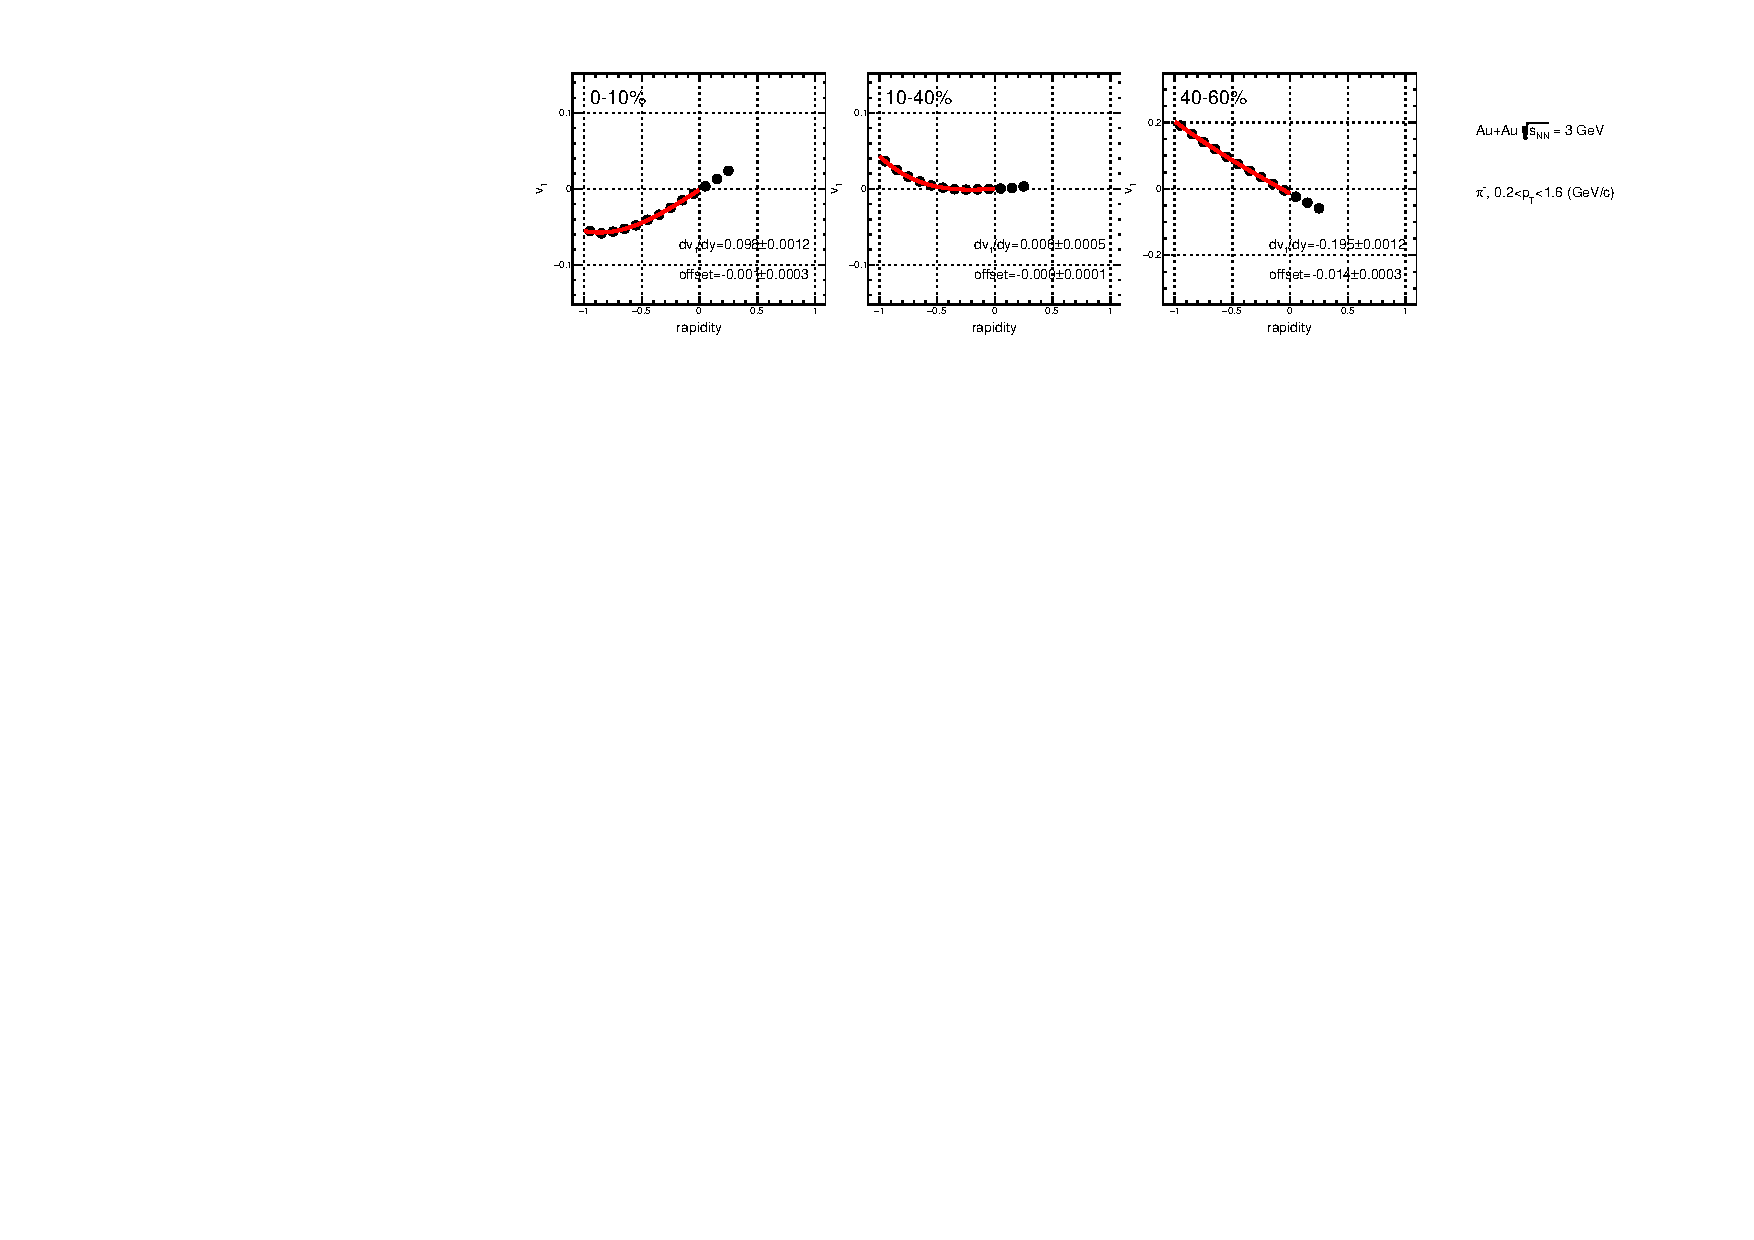
\includegraphics[scale=0.8]{FXT3gev/chapter3/fig/v1ypikp/pionm_v1y_wide_cent.pdf}
\caption{\label{pion_dv1y_widecent} pions' $v_{1}$ as a function of rapidity(y) in Au+Au collision at $\sqrt{s_{NN}}$=3GeV in 0-10\%, 10-40\% and 40-60\% bins.}
\end{figure}

\clearpage

Figure \ref{pion_dv1pt_widecent} shows the  $\pi^{+}$ and $\pi^{-}$ $v_{1}$ slope as a function of $p_{T}$, the fitting formula is from \ref{fit_v1_formula}, which is performed in each $p_{T}$ bin to extract the $v_{1}$ slope. As we can see, the $v_{1}$ slope increases with $p_{T}$ increasing.

\begin{figure}[h]
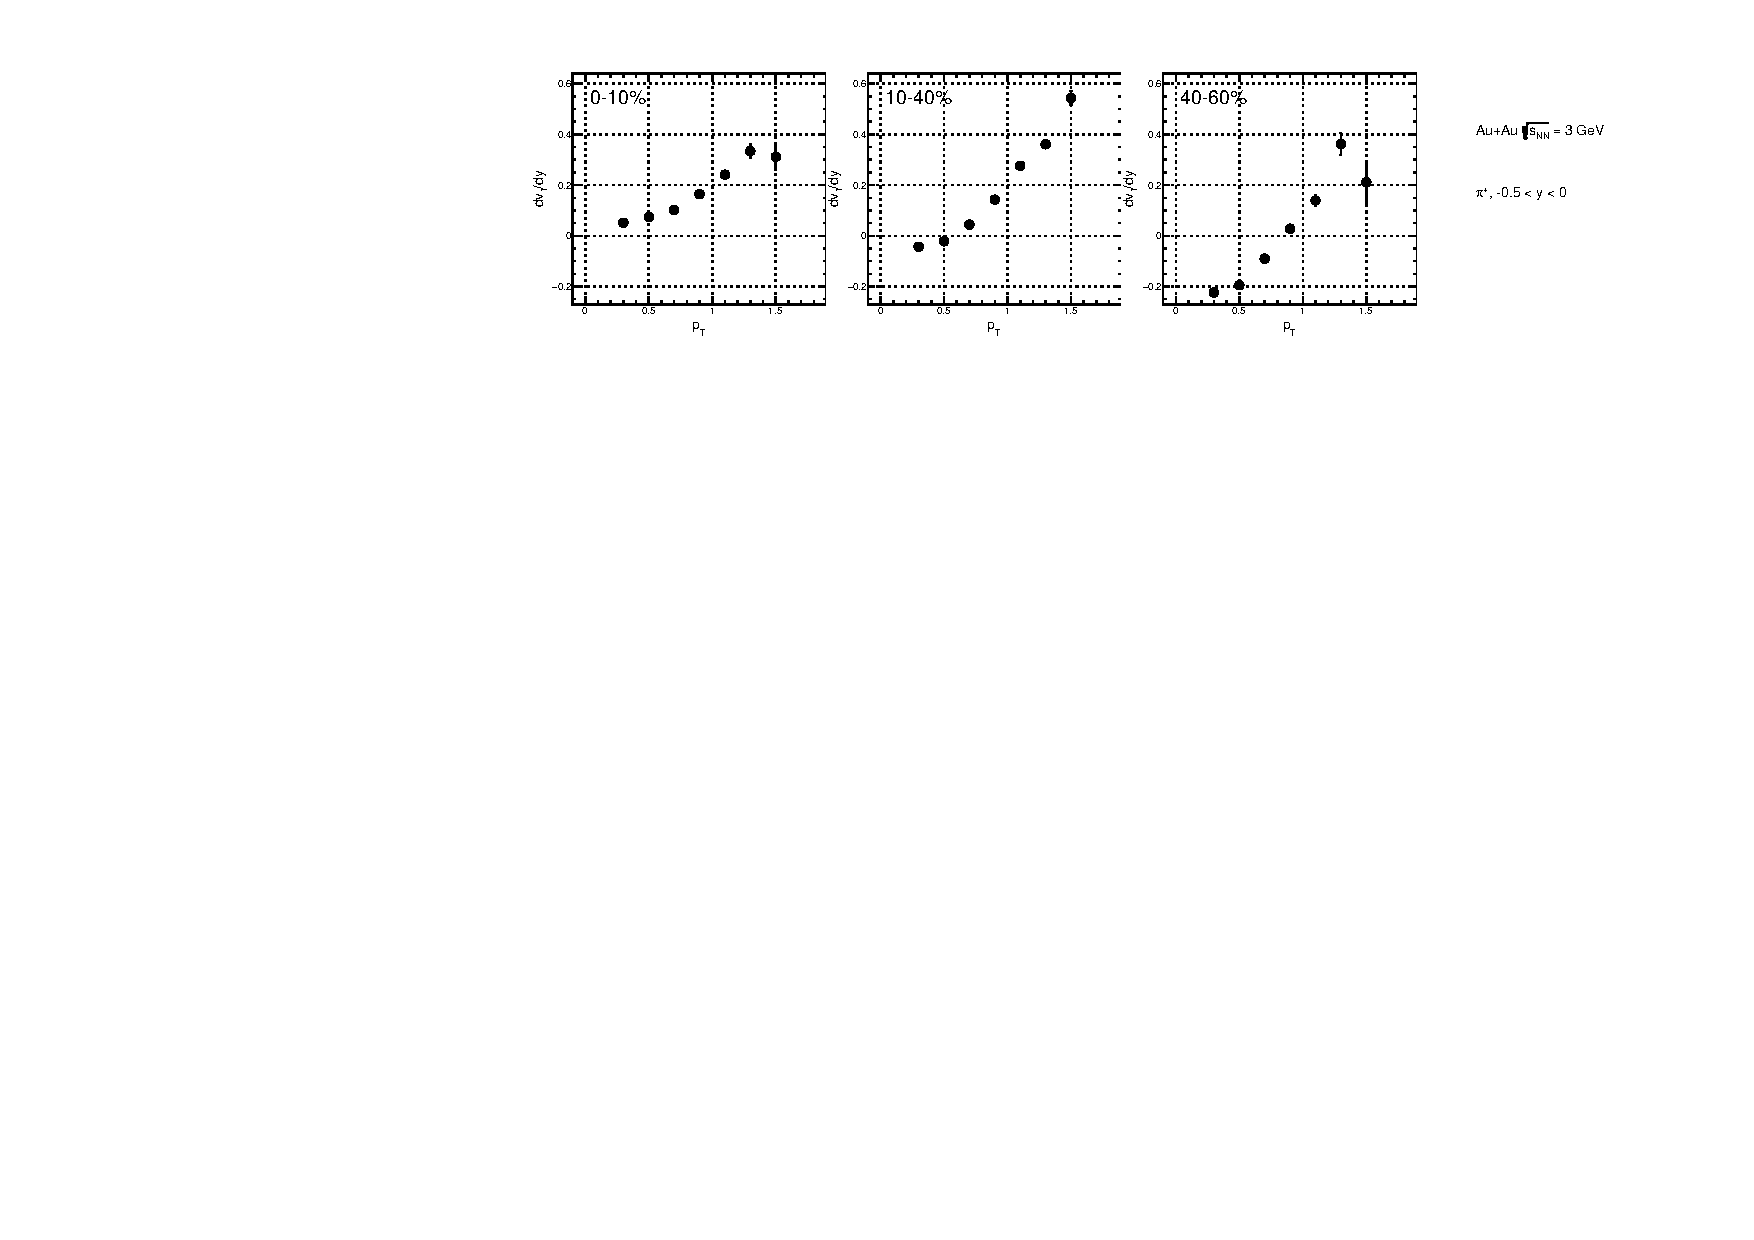
\includegraphics[scale=0.5]{FXT3gev/chapter3/fig/v1ptpikp/pip_dv1pt_widecent.pdf}
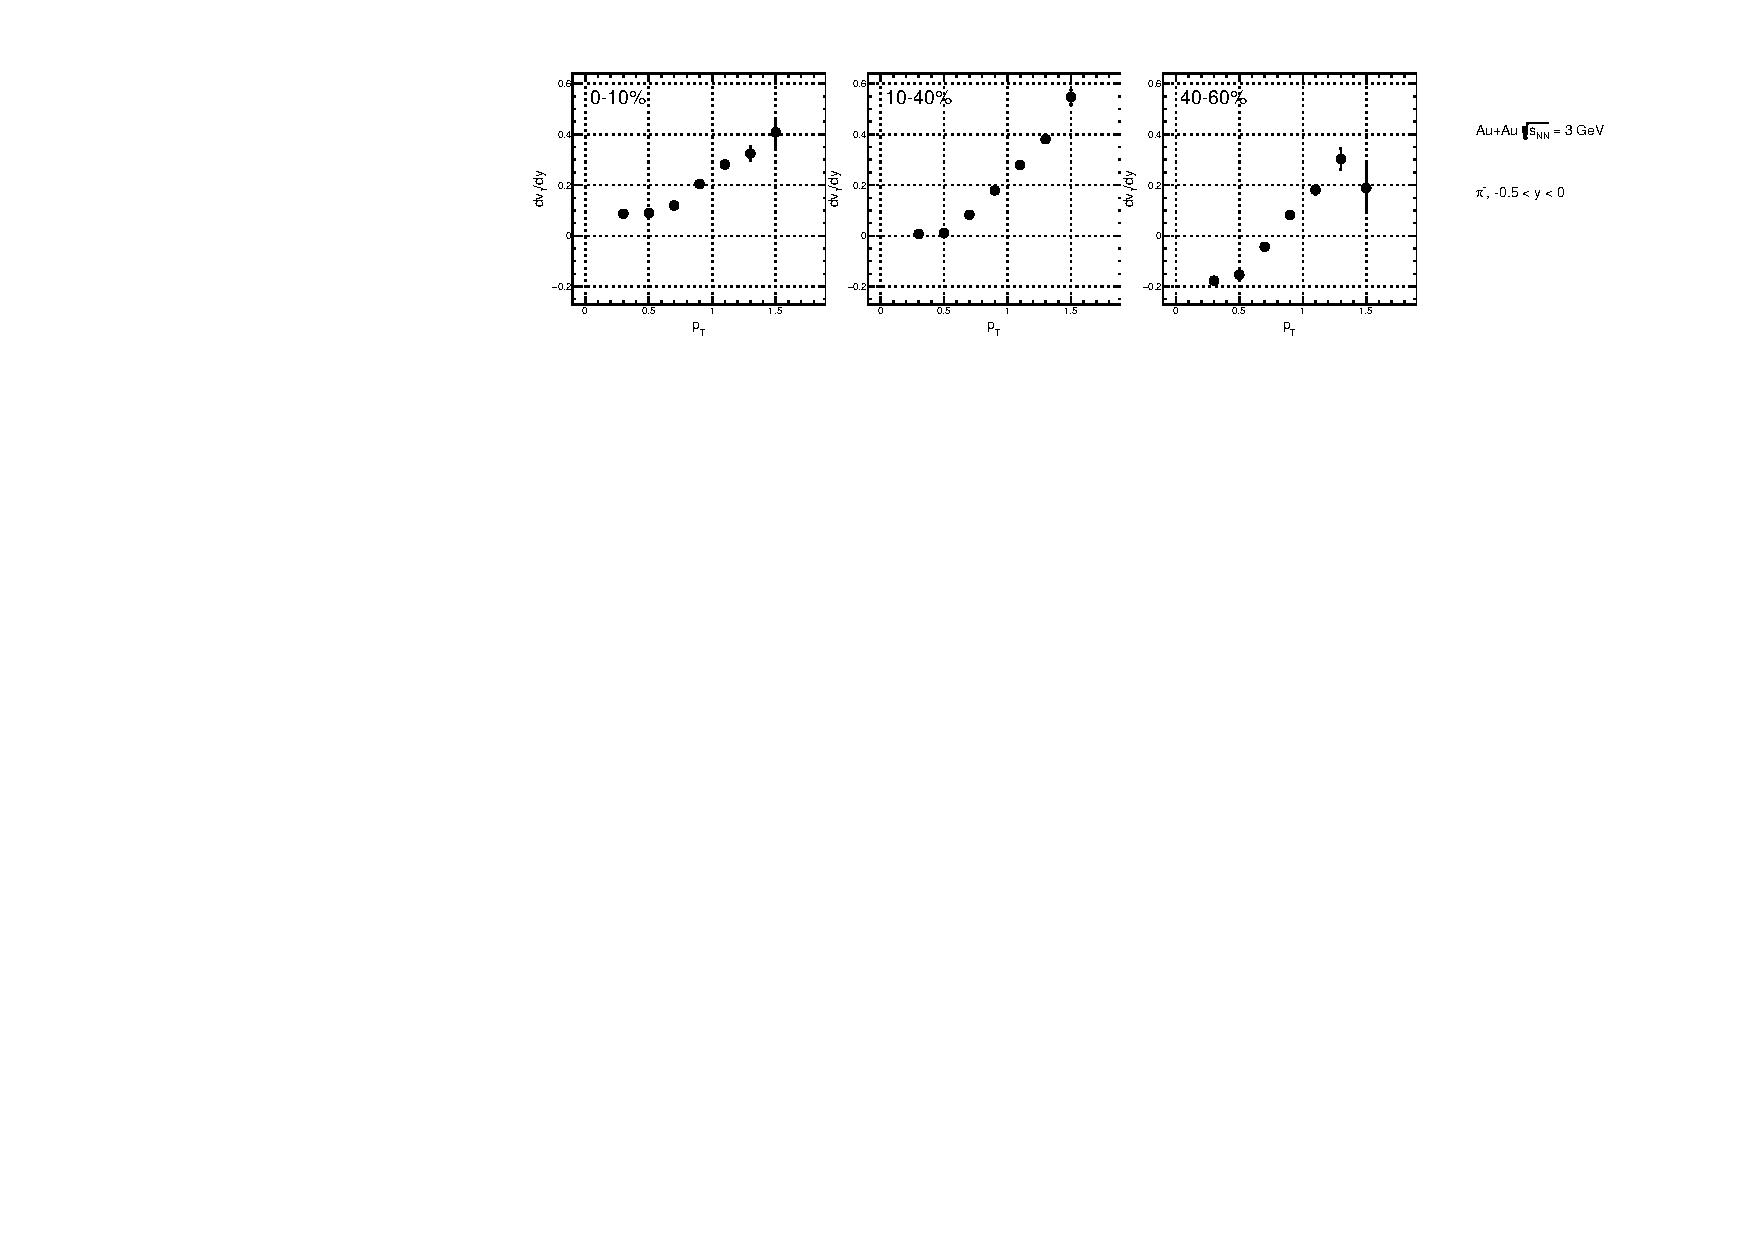
\includegraphics[scale=0.5]{FXT3gev/chapter3/fig/v1ptpikp/pim_dv1pt_widecent.pdf}
\caption{pions' $dv_{1}/dy$ as a function of transverse momentum ($p_{T}$) in Au+Au collisions at $\sqrt{s_{NN}}$ = 3 GeV in 0-10\%, 10-40\% and 40-60\% centrality bins.}
\label{pion_dv1pt_widecent}
\end{figure}

\clearpage

\subsubsection{kaons' $v_{1}$ as a function of $p_{T}$ and rapidity}
Figure \ref{kaon_v1y_cent} shows $K^{+}, K^{-}$ $v_{1}$ as a function of y for different centrality bins from 0-5\% to 50-60\%, The red line is fitting function \ref{fit_v1_formula}, $p_{T}$ range is [0.4, 1.6] GeV/c, which is same with STAR BES-I results. As we can see, the magnitude of kaons' $v_{1}$ has weak centrality dependence, which is not same with pions' case, this might be due to kaon has smaller hadronic scattering cross section than pions, and the $v_{1}$ between $K^{+}$ and $K^{-}$ is very similar, figure \ref{kaon_dv1dy_cent} shows $K^{+}, K^{-}$ $dv_{1}/dy$ as a function of centrality. In order to make comparison to STAR BES-I results, we have these results in wider centrality bin in the figure \ref{kaon_v1y_widecent}. And their $v_{1}$ slope is decreasing from central collision to peripheral collision.


\begin{figure}[h]
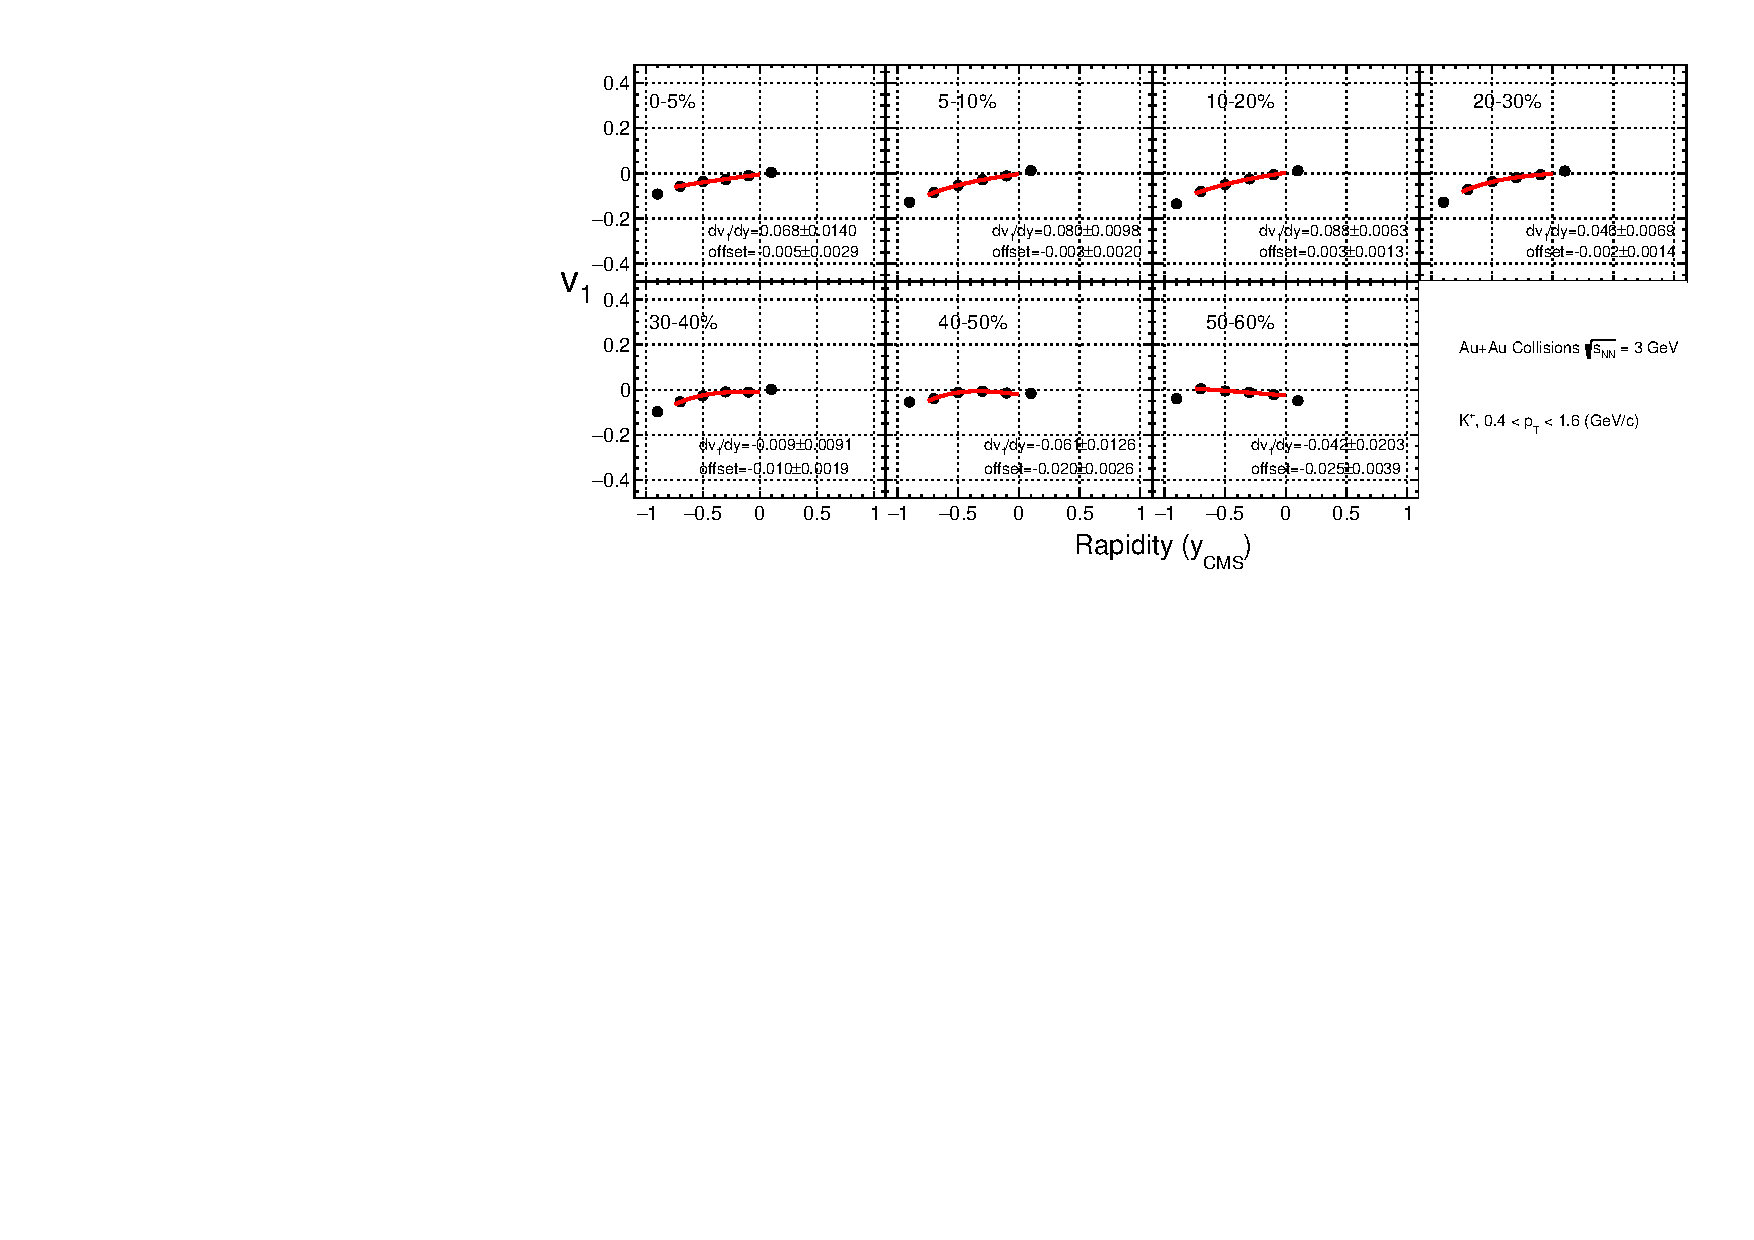
\includegraphics[scale=0.5]{chapter3/fig/v1ypikp/v1kaonp_cent.pdf}
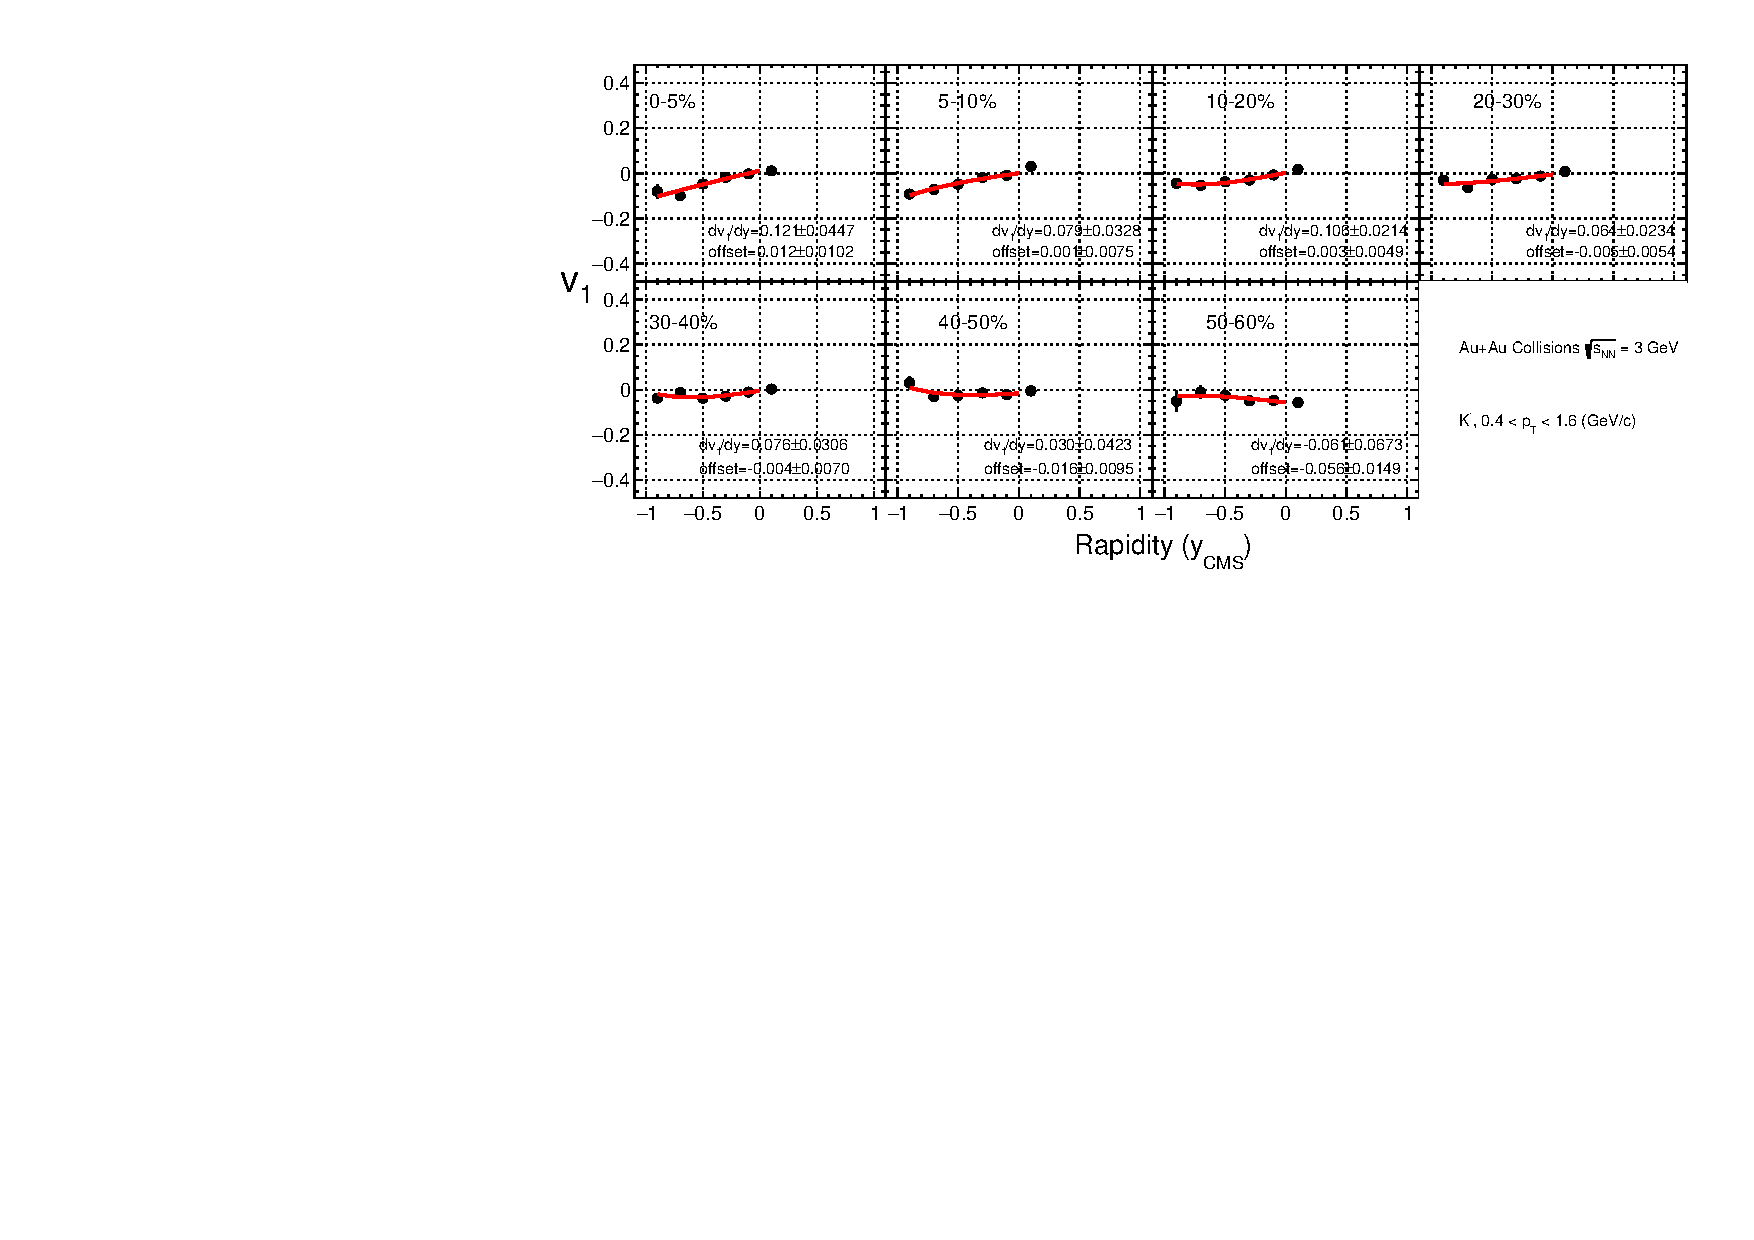
\includegraphics[scale=0.5]{chapter3/fig/v1ypikp/v1kaonm_cent.pdf}
\caption{\label{kaon_v1y_cent} $v_{1}$ as a function of rapidity(y) in different centrality bins for $K^{+}$ and $K^{-}$ in Au+Au collisions at $\sqrt{s_{NN}}$. The red line is fitting function.}
\end{figure}

\begin{figure}[h]
\centering
\subfigure{   
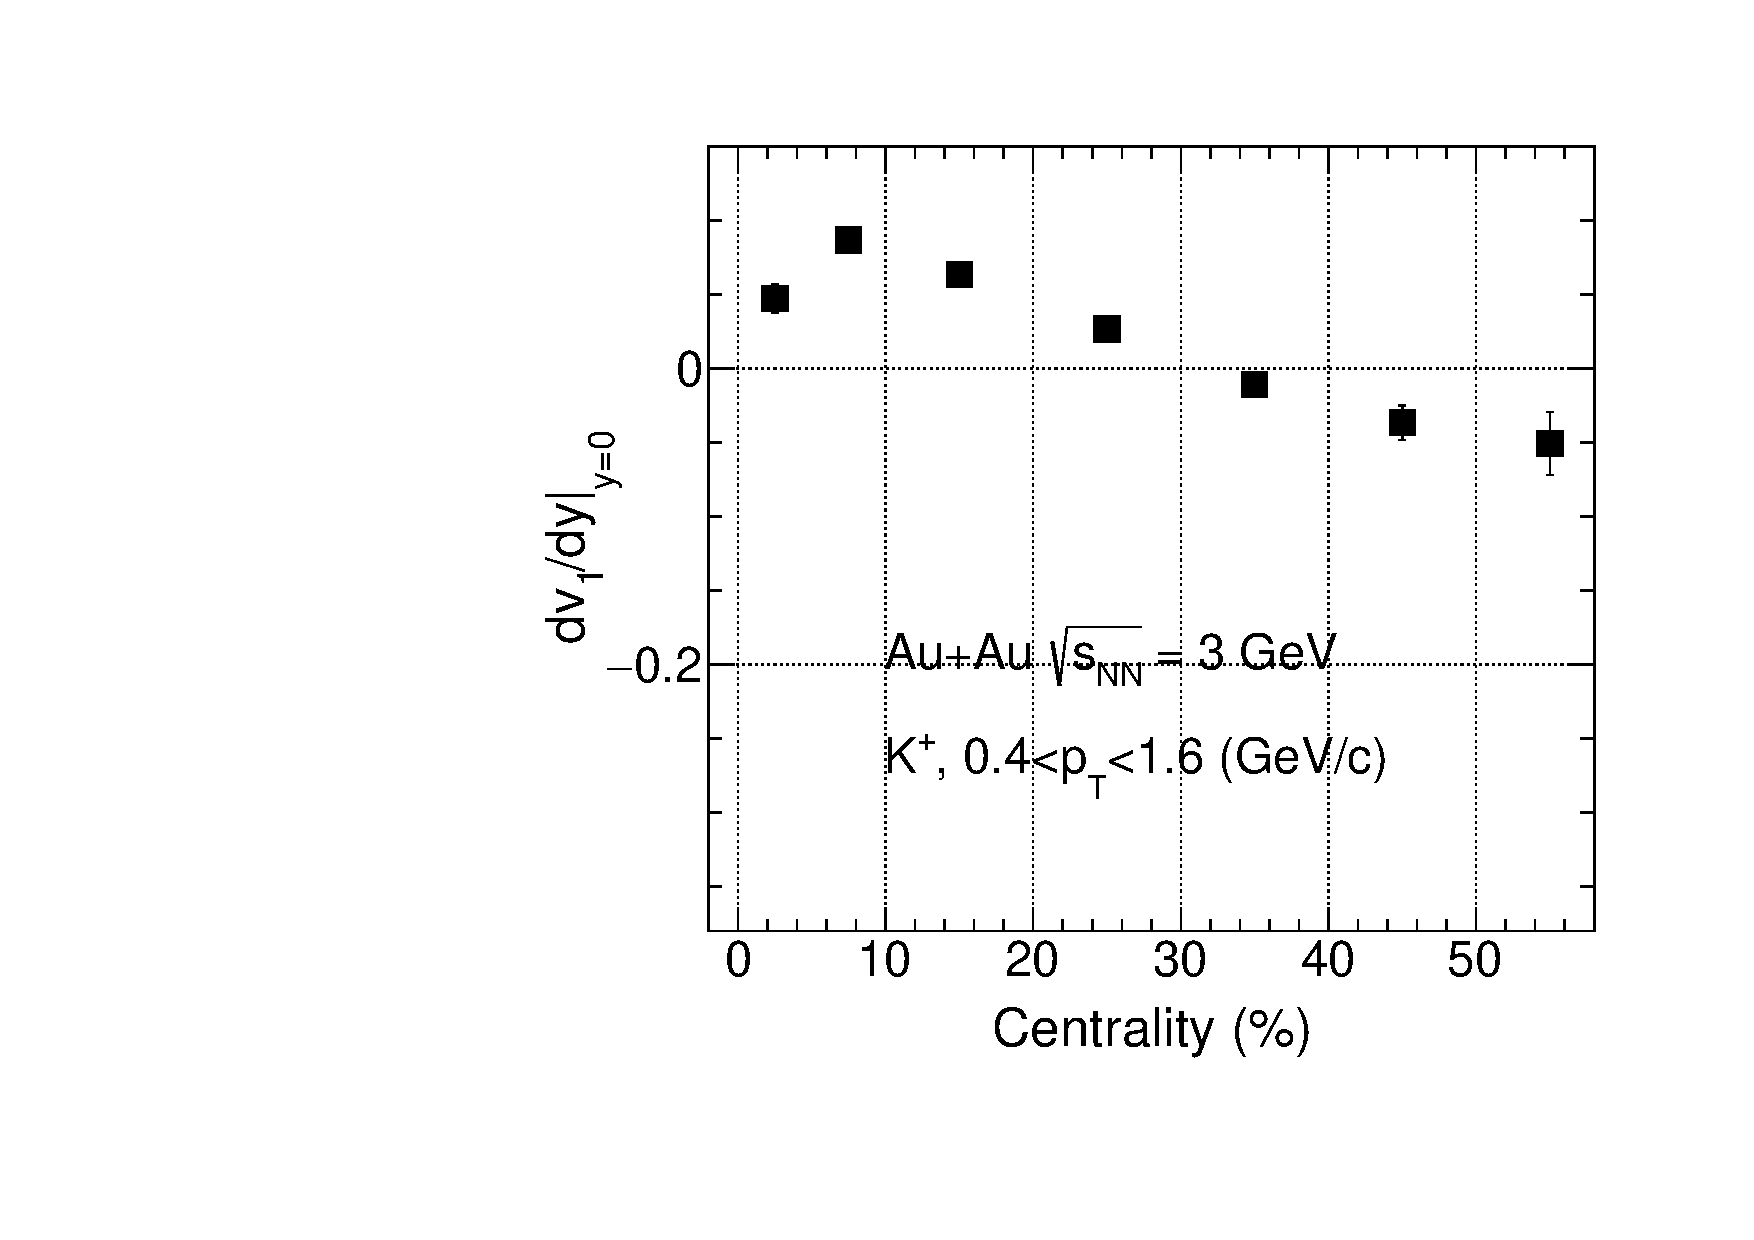
\includegraphics[width=0.4\textwidth]{chapter3/fig/v1ypikp/dv1dy_kaonp.pdf}}
\subfigure{
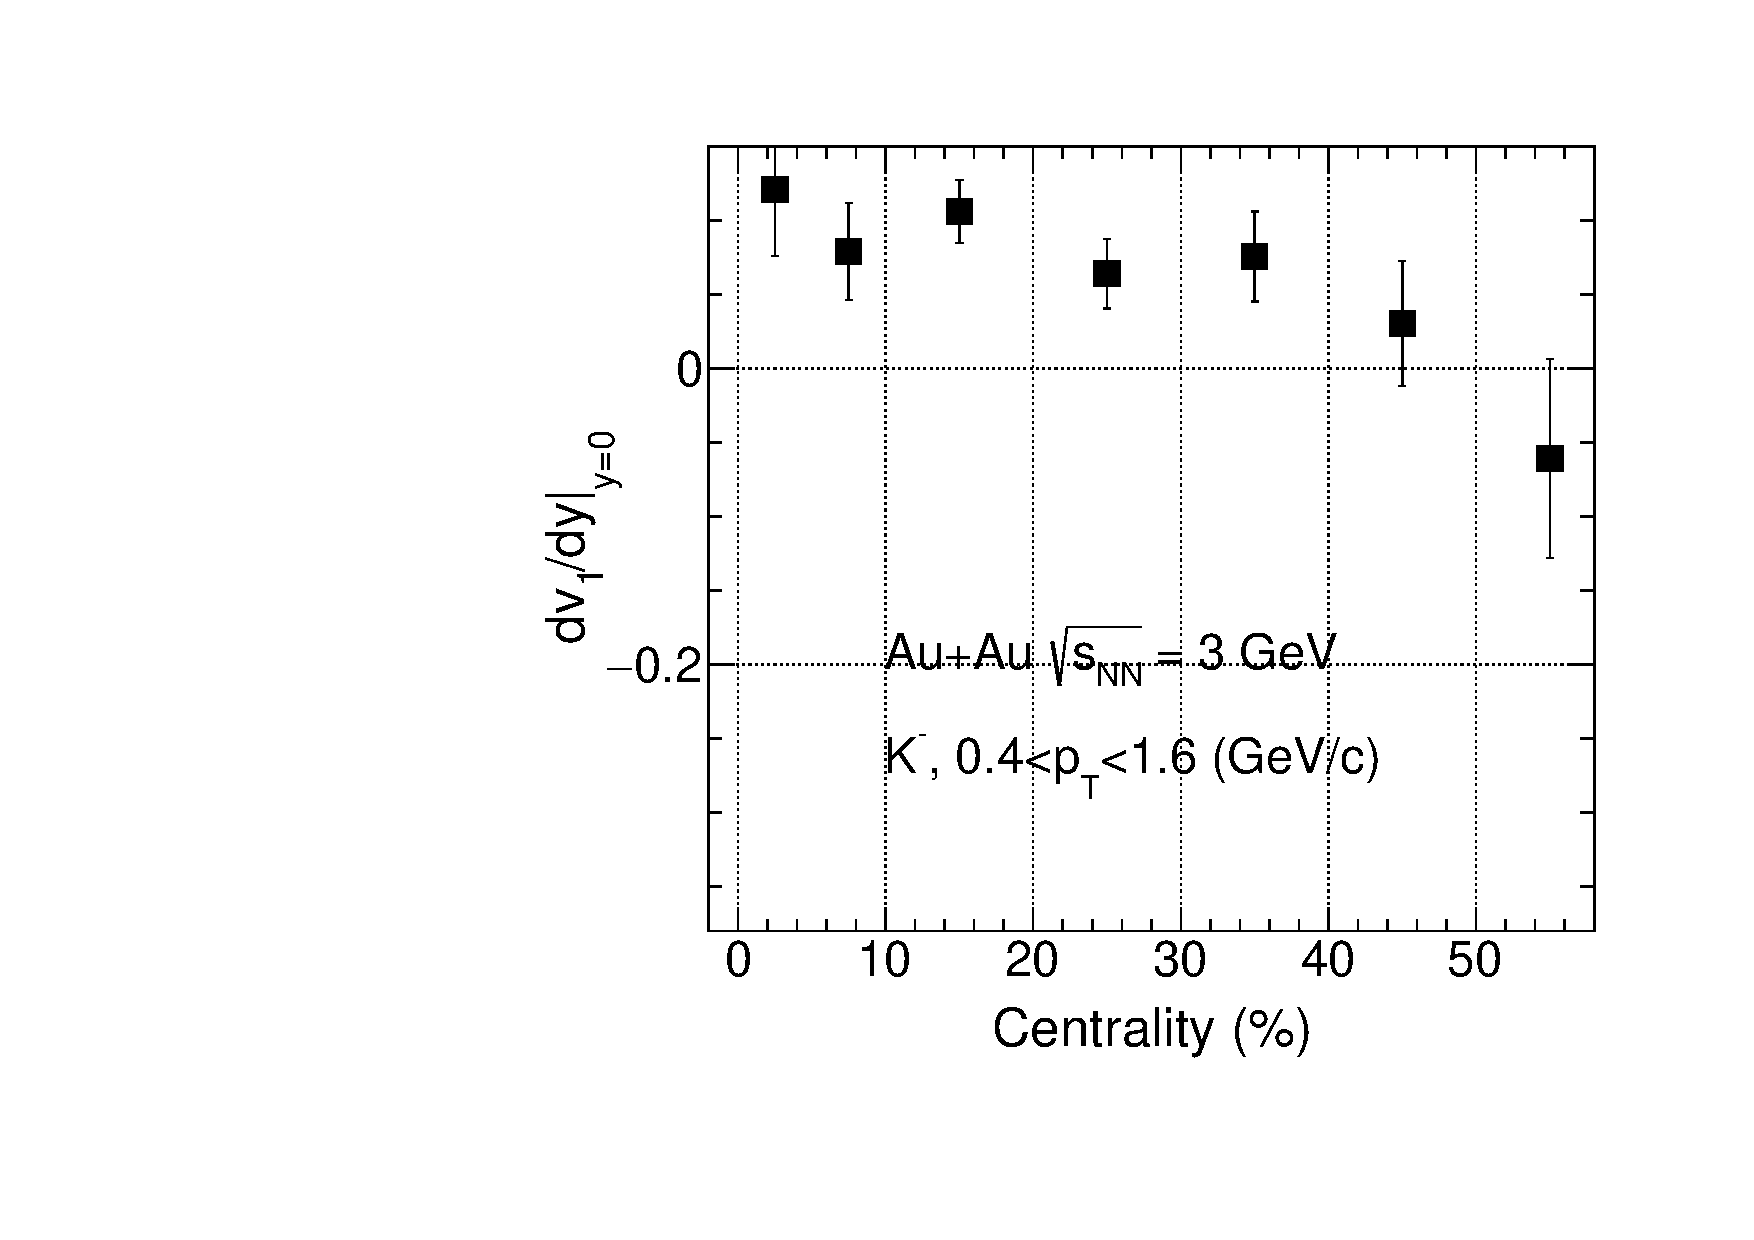
\includegraphics[width=0.4\textwidth]{chapter3/fig/v1ypikp/dv1dy_kaonm.pdf}}
\caption{\label{kaon_dv1dy_cent} kaons' $v_{1}$ slope $dv_{1}/dy$ as a function of centrality, (left) $K^{+}$ (right) $K^{-}$ in Au+Au collisions $\sqrt{s_{NN}}$ = 3GeV.}
\end{figure}

\begin{figure}[h]
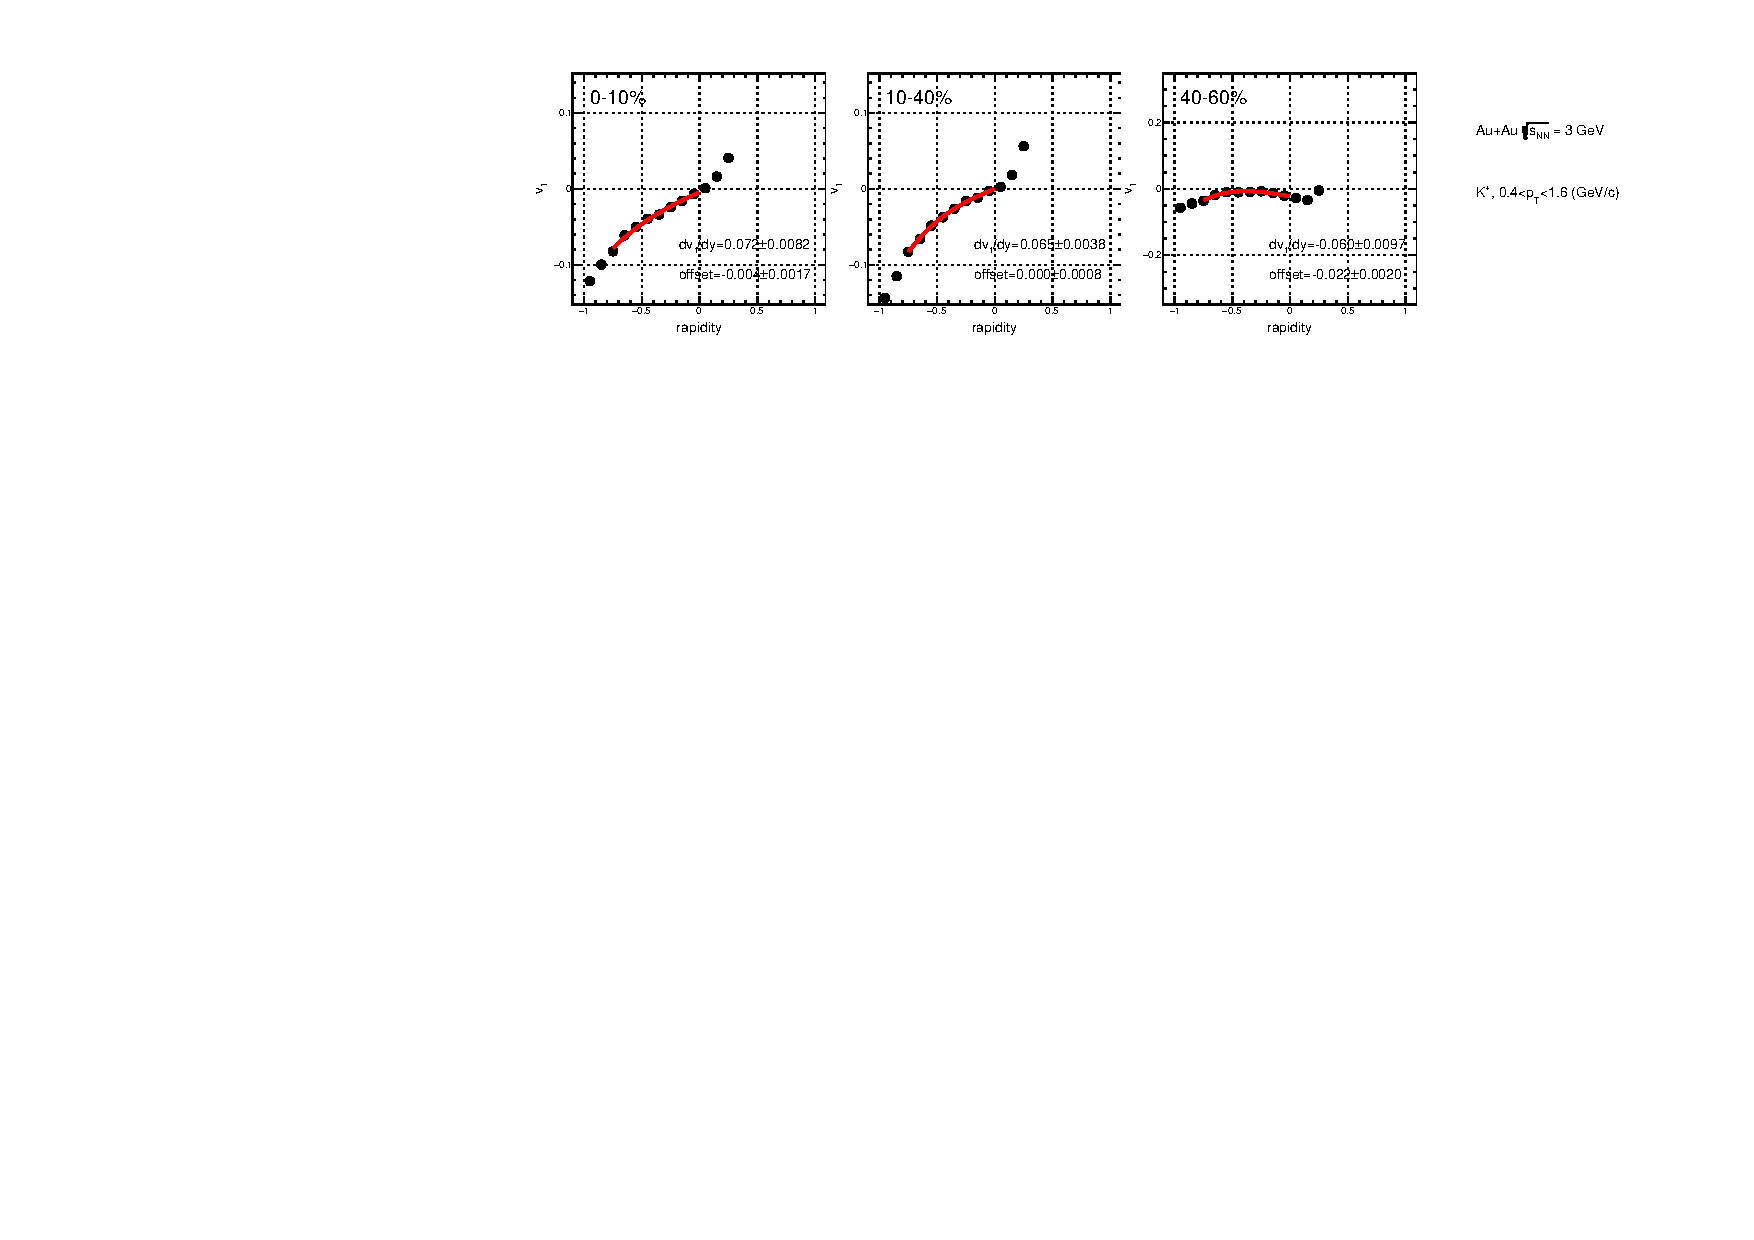
\includegraphics[scale=0.8]{chapter3/fig/v1ypikp/kaonp_v1y_wide_cent.pdf}
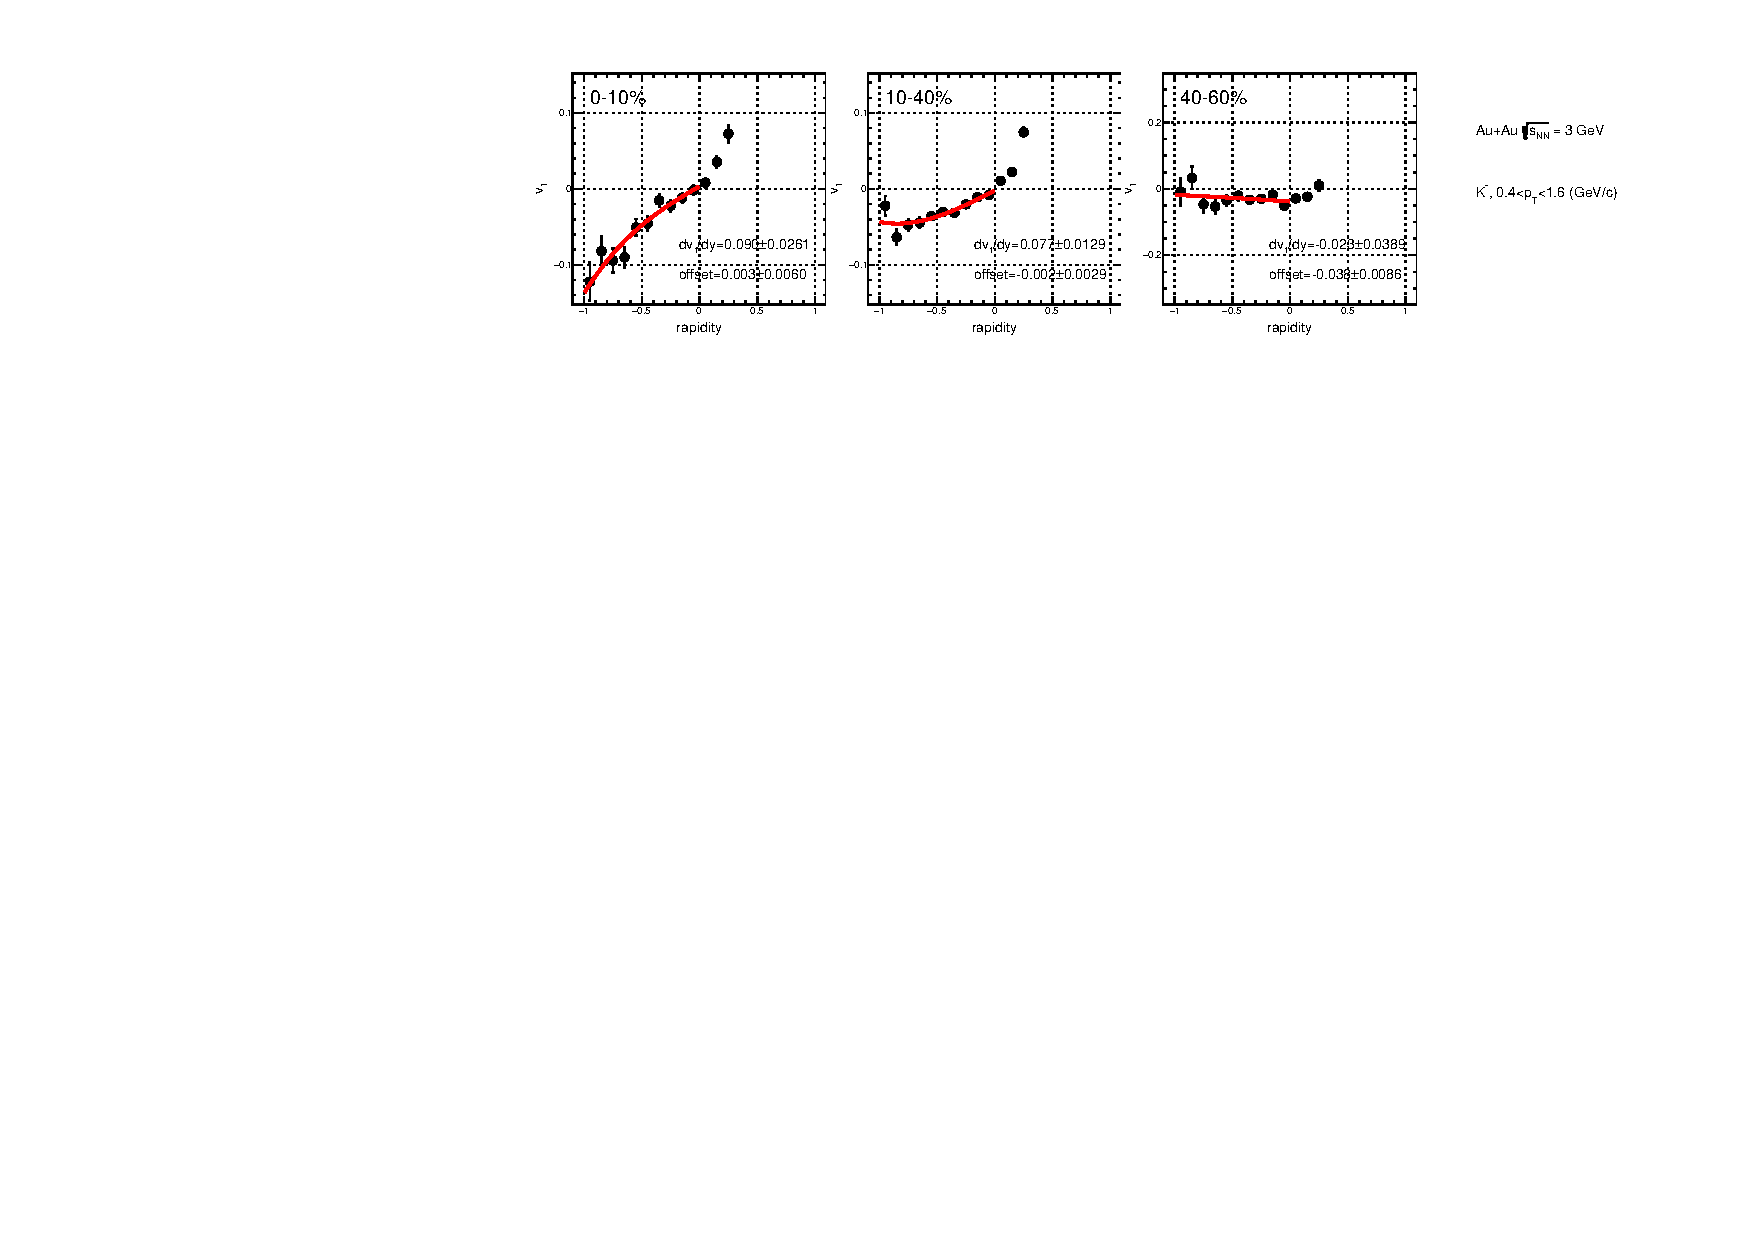
\includegraphics[scale=0.8]{chapter3/fig/v1ypikp/kaonm_v1y_wide_cent.pdf}
\caption{\label{kaon_v1y_widecent} kaons' $v_{1}$ as a function of rapidity(y) in Au+Au collision at $\sqrt{s_{NN}}$=3GeV in 0-10\%, 10-40\% and 40-60\% bins.}
\end{figure}

\clearpage

Figure \ref{kaon_dv1pt_widecent} shows the  $K^{+}$ and $K^{-}$ $v_{1}$ slope as a function of $p_{T}$, the fitting formula is from \ref{fit_v1_formula}, which is performed in each $p_{T}$ bin to extract the $v_{1}$ slope. As we can see, the $v_{1}$ slope increases with $p_{T}$ increasing.

\begin{figure}[h]
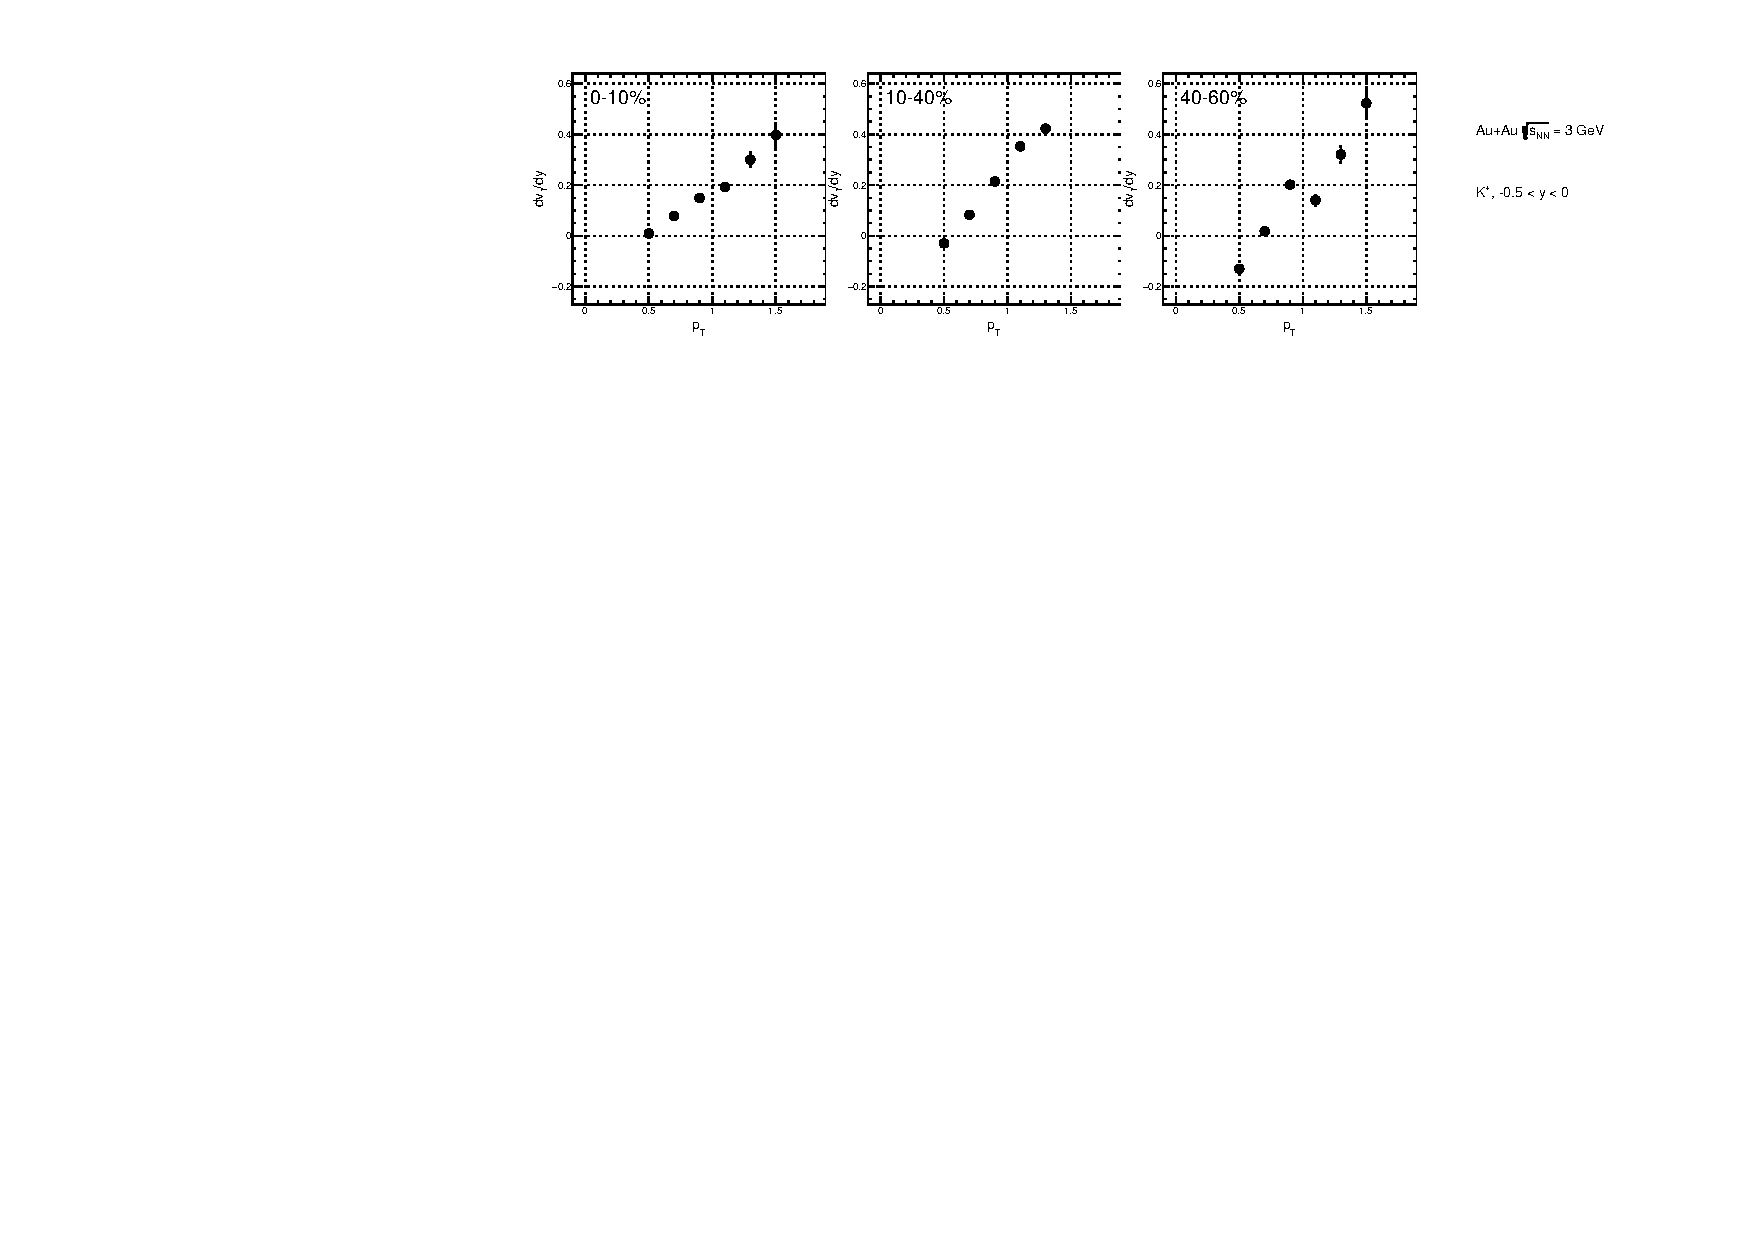
\includegraphics[scale=0.5]{FXT3gev/chapter3/fig/v1ptpikp/kap_dv1pt_widecent.pdf}
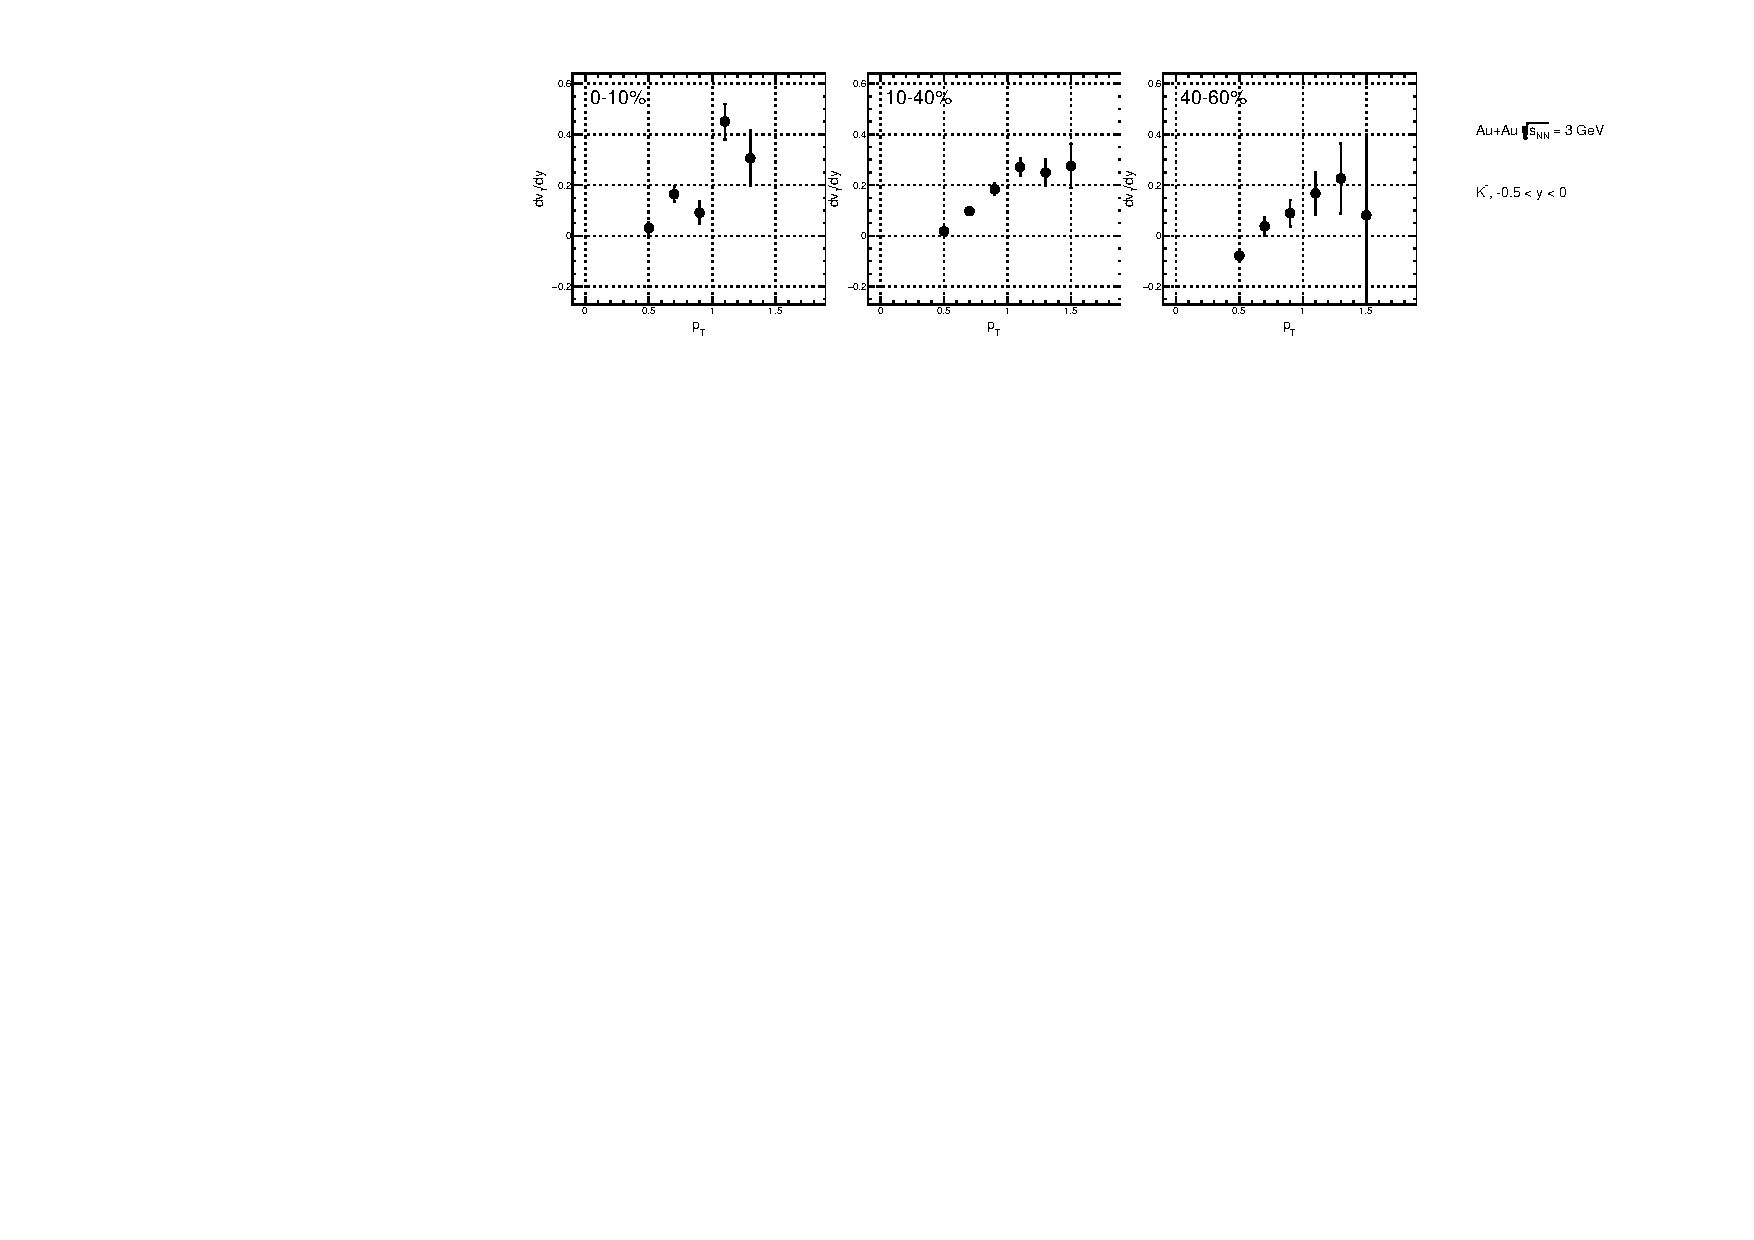
\includegraphics[scale=0.5]{FXT3gev/chapter3/fig/v1ptpikp/kam_dv1pt_widecent.pdf}
\caption{kaons' $dv_{1}/dy$ as a function of transverse momentum ($p_{T}$) in Au+Au collisions at $\sqrt{s_{NN}}$ = 3 GeV in 0-10\%, 10-40\% and 40-60\% centrality bins.}
\label{kaon_dv1pt_widecent}
\end{figure}

\clearpage

\subsubsection{proton $v_{1}$ as a function of $p_{T}$ and rapidity}
In this chapter, we will show the results of proton $v_{1}$ as a function of $p_{T}$ and rapidity(y). 
Figure \ref{proton_v1y_cent} shows proton $v_{1}$ as a function of y for different centrality bins from 0-5\% to 50-60\%, The red line is fitting function \ref{fit_v1_formula}, $p_{T}$ range is [0.4, 2.0] GeV/c, which is same with STAR BES-I results. As we can see, the magnitude of proton's $v_{1}$ has centrality dependence, figure \ref{proton_dv1dy_cent} shows proton $dv_{1}/dy$ as a function of centrality. In order to make comparison to STAR BES-I results, we have these results in wider centrality bin in the figure \ref{proton_v1y_widecent}. And the $v_{1}$ slope has maximum value in the mid-central collision.


\begin{figure}[h]
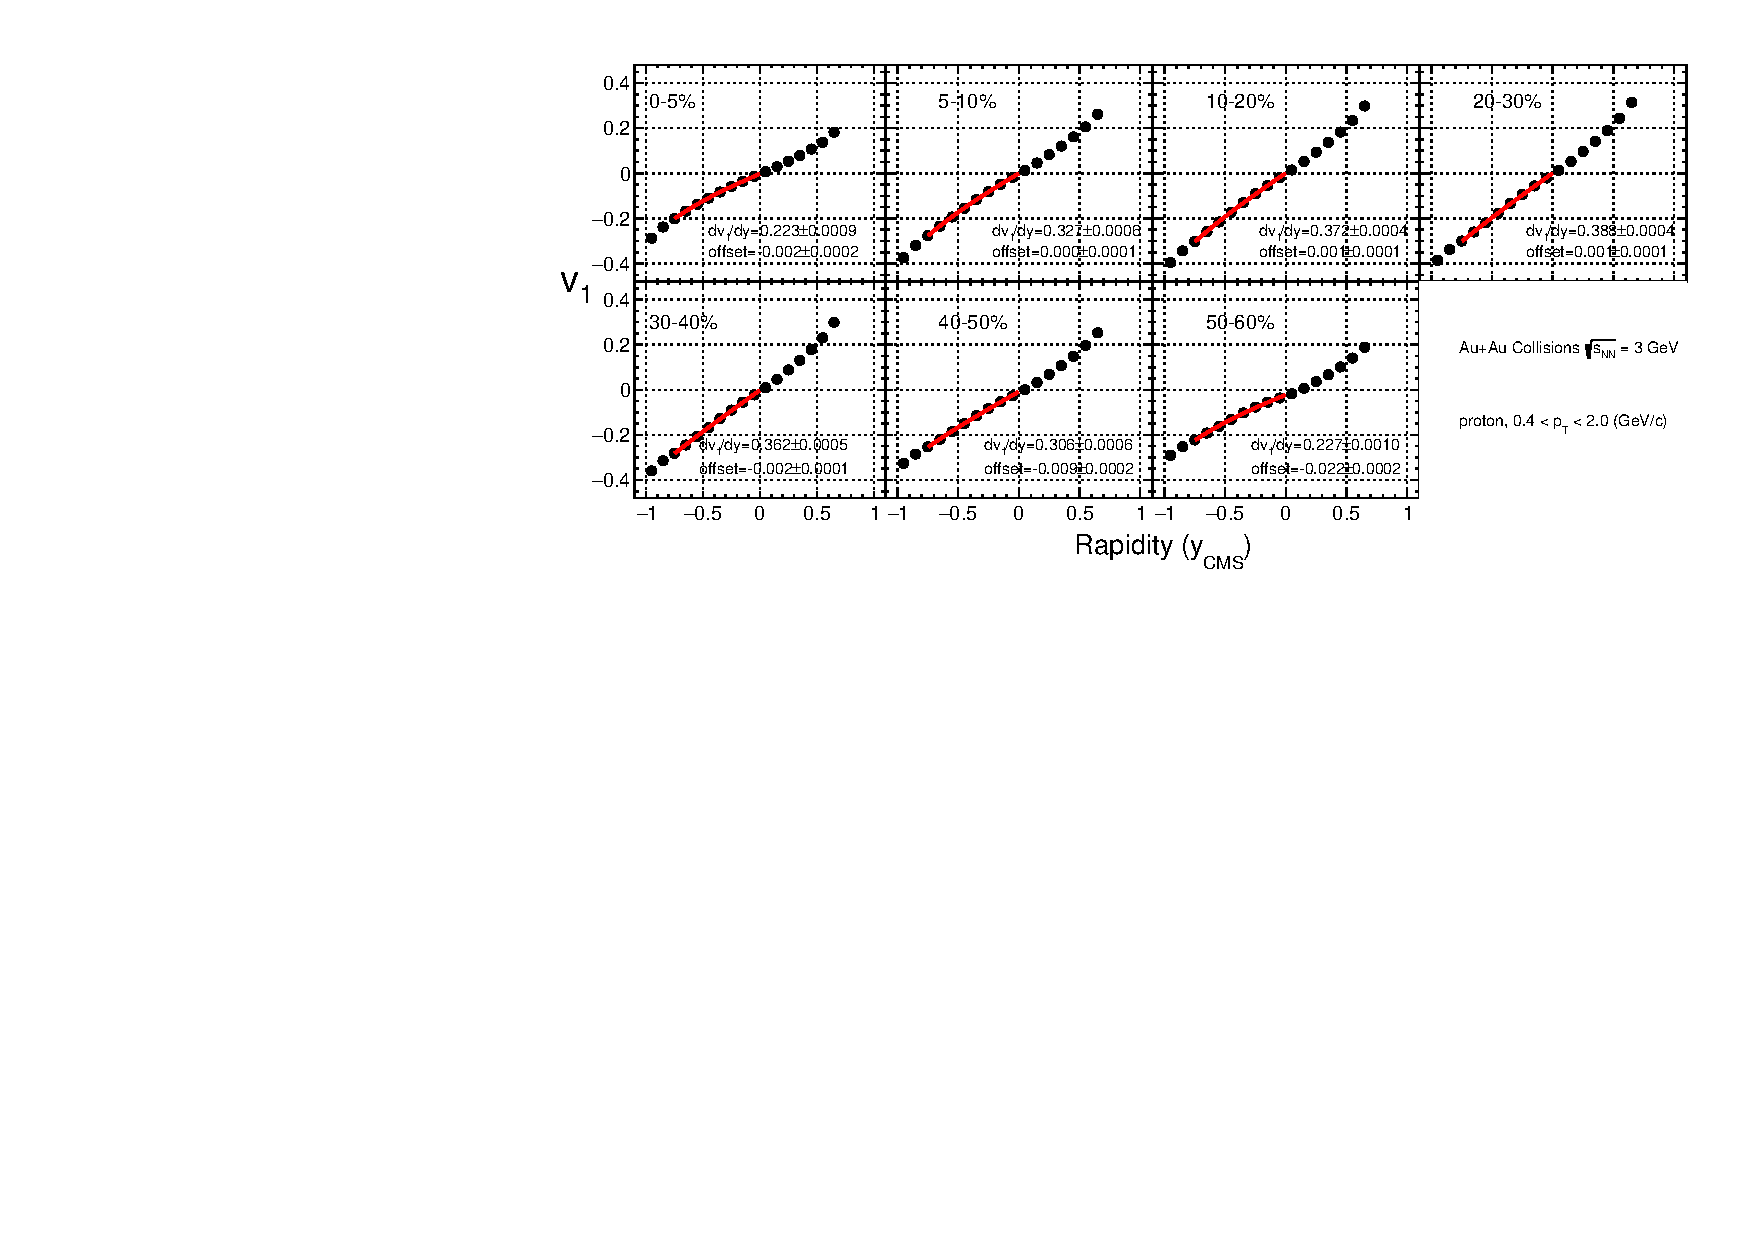
\includegraphics[scale=0.8]{chapter3/fig/v1ypikp/v1proton_cent.pdf}
\caption{\label{proton_v1y_cent} $v_{1}$ as a function of rapidity(y) in different centrality bins for proton in Au+Au collisions at $\sqrt{s_{NN}}$. The red line is fitting function.}
\end{figure}

\begin{figure}[h]
\centering
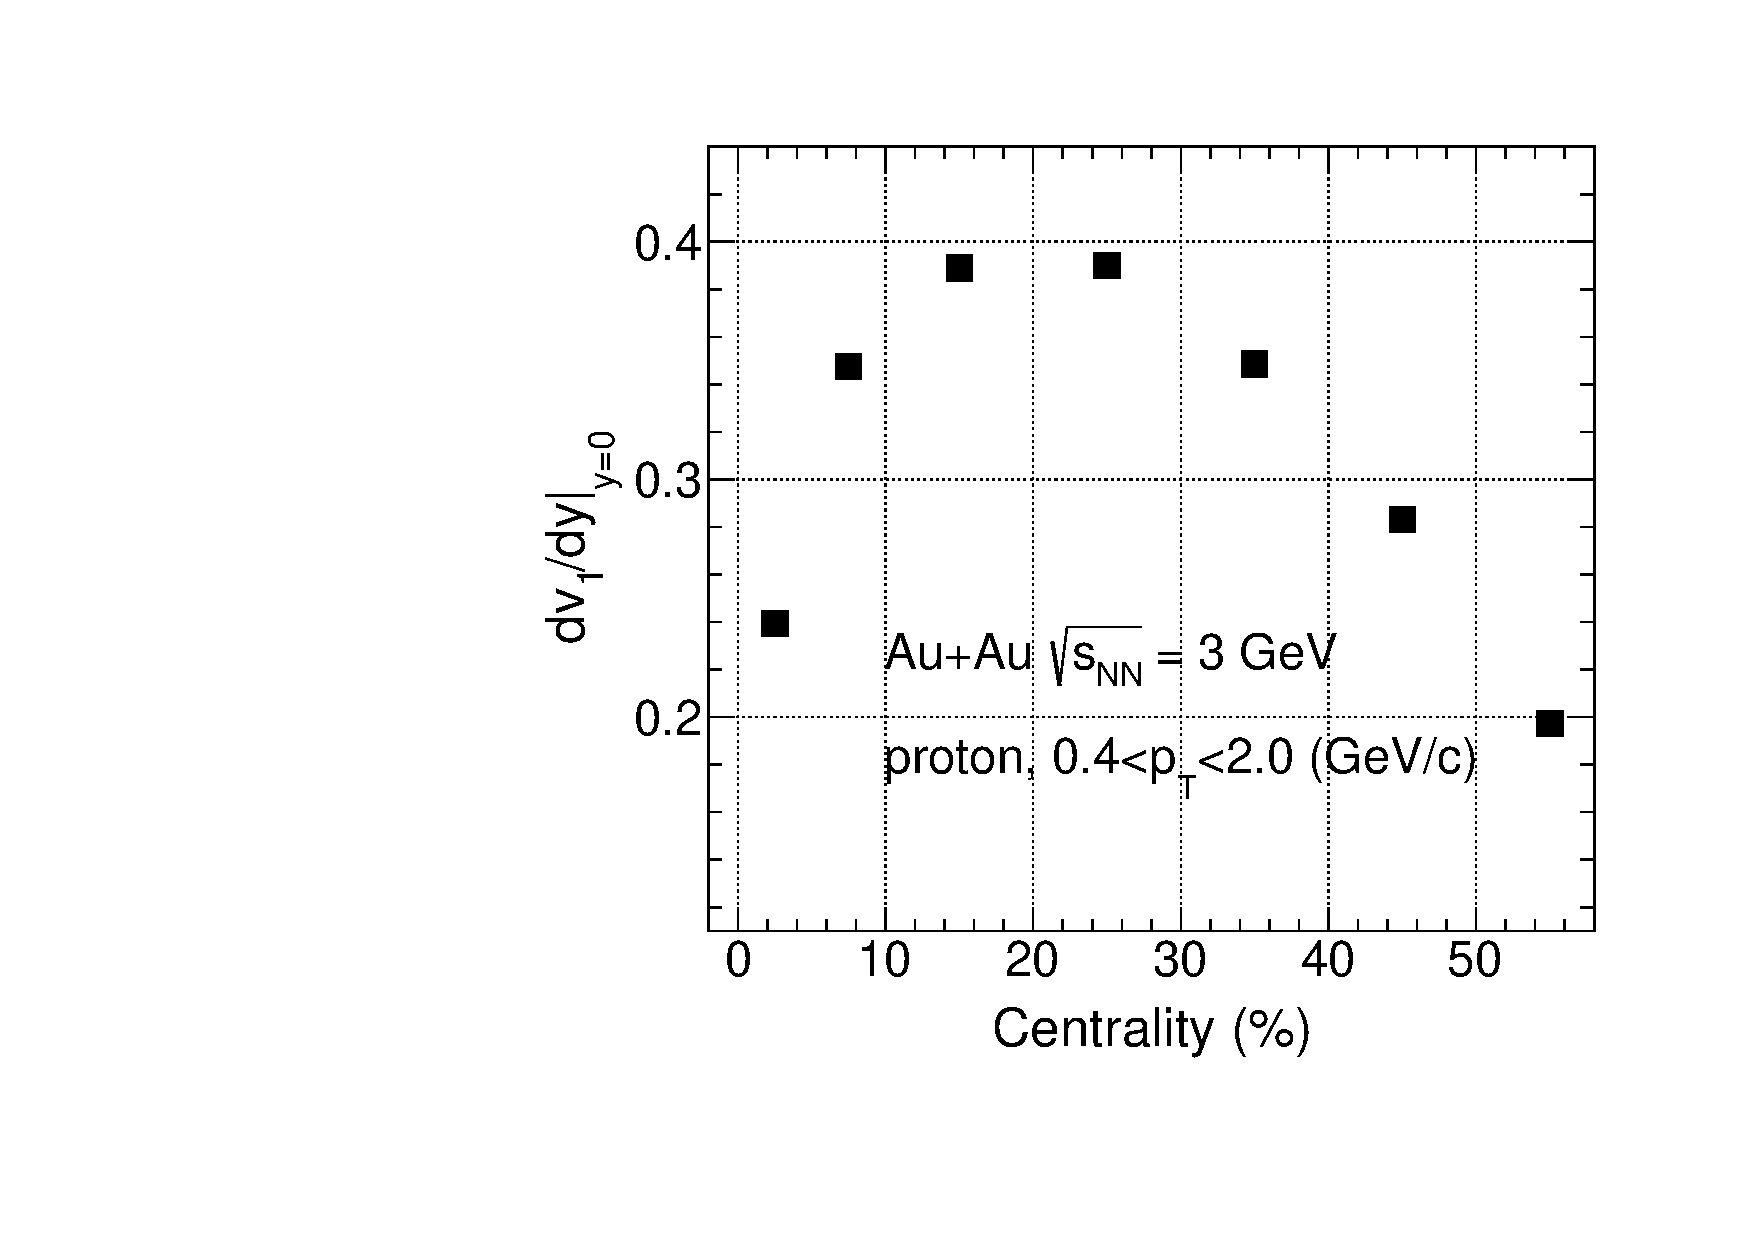
\includegraphics[scale=0.5]{chapter3/fig/v1ypikp/dv1dy_proton.pdf}
\caption{\label{kaon_dv1dy_cent} protons' $v_{1}$ slope $dv_{1}/dy$ as a function of centrality in Au+Au collisions $\sqrt{s_{NN}}$ = 3GeV.}
\end{figure}

\begin{figure}[h]
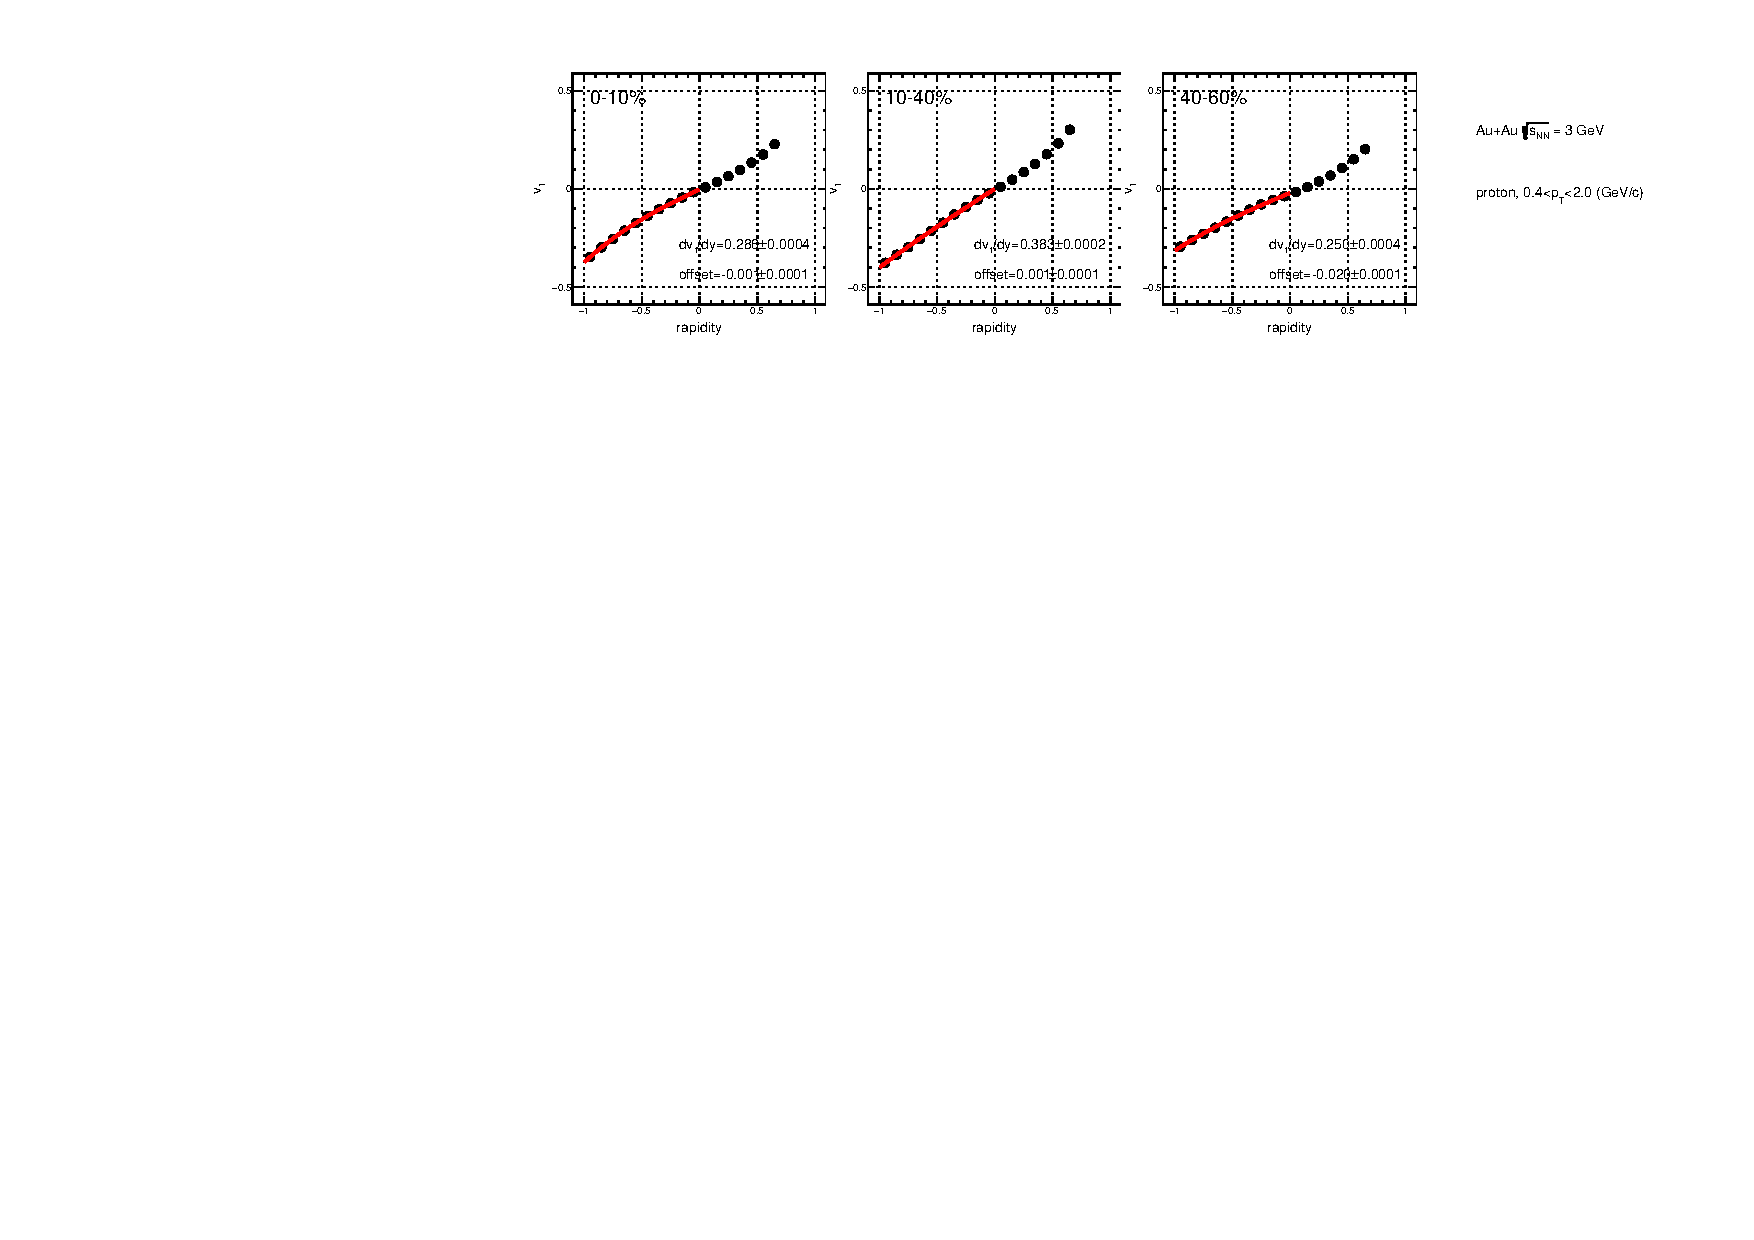
\includegraphics[scale=0.8]{chapter3/fig/v1ypikp/protonp_v1y_wide_cent.pdf}
\caption{\label{proton_v1y_widecent} protons' $v_{1}$ as a function of rapidity(y) in Au+Au collision at $\sqrt{s_{NN}}$=3GeV in 0-10\%, 10-40\% and 40-60\% bins.}
\end{figure}

\clearpage

We also study the $p_{T}$ dependence of protons' $v_{1}$ in the mid-rapidity region (-0.5$<$y$<$0) in different centrality bins in the figure \ref{proton_dv1pt_widecent}. As we can see, proton's $v_{1}$ slope increases with $p_{T}$ increasing. 



\begin{figure}[h]
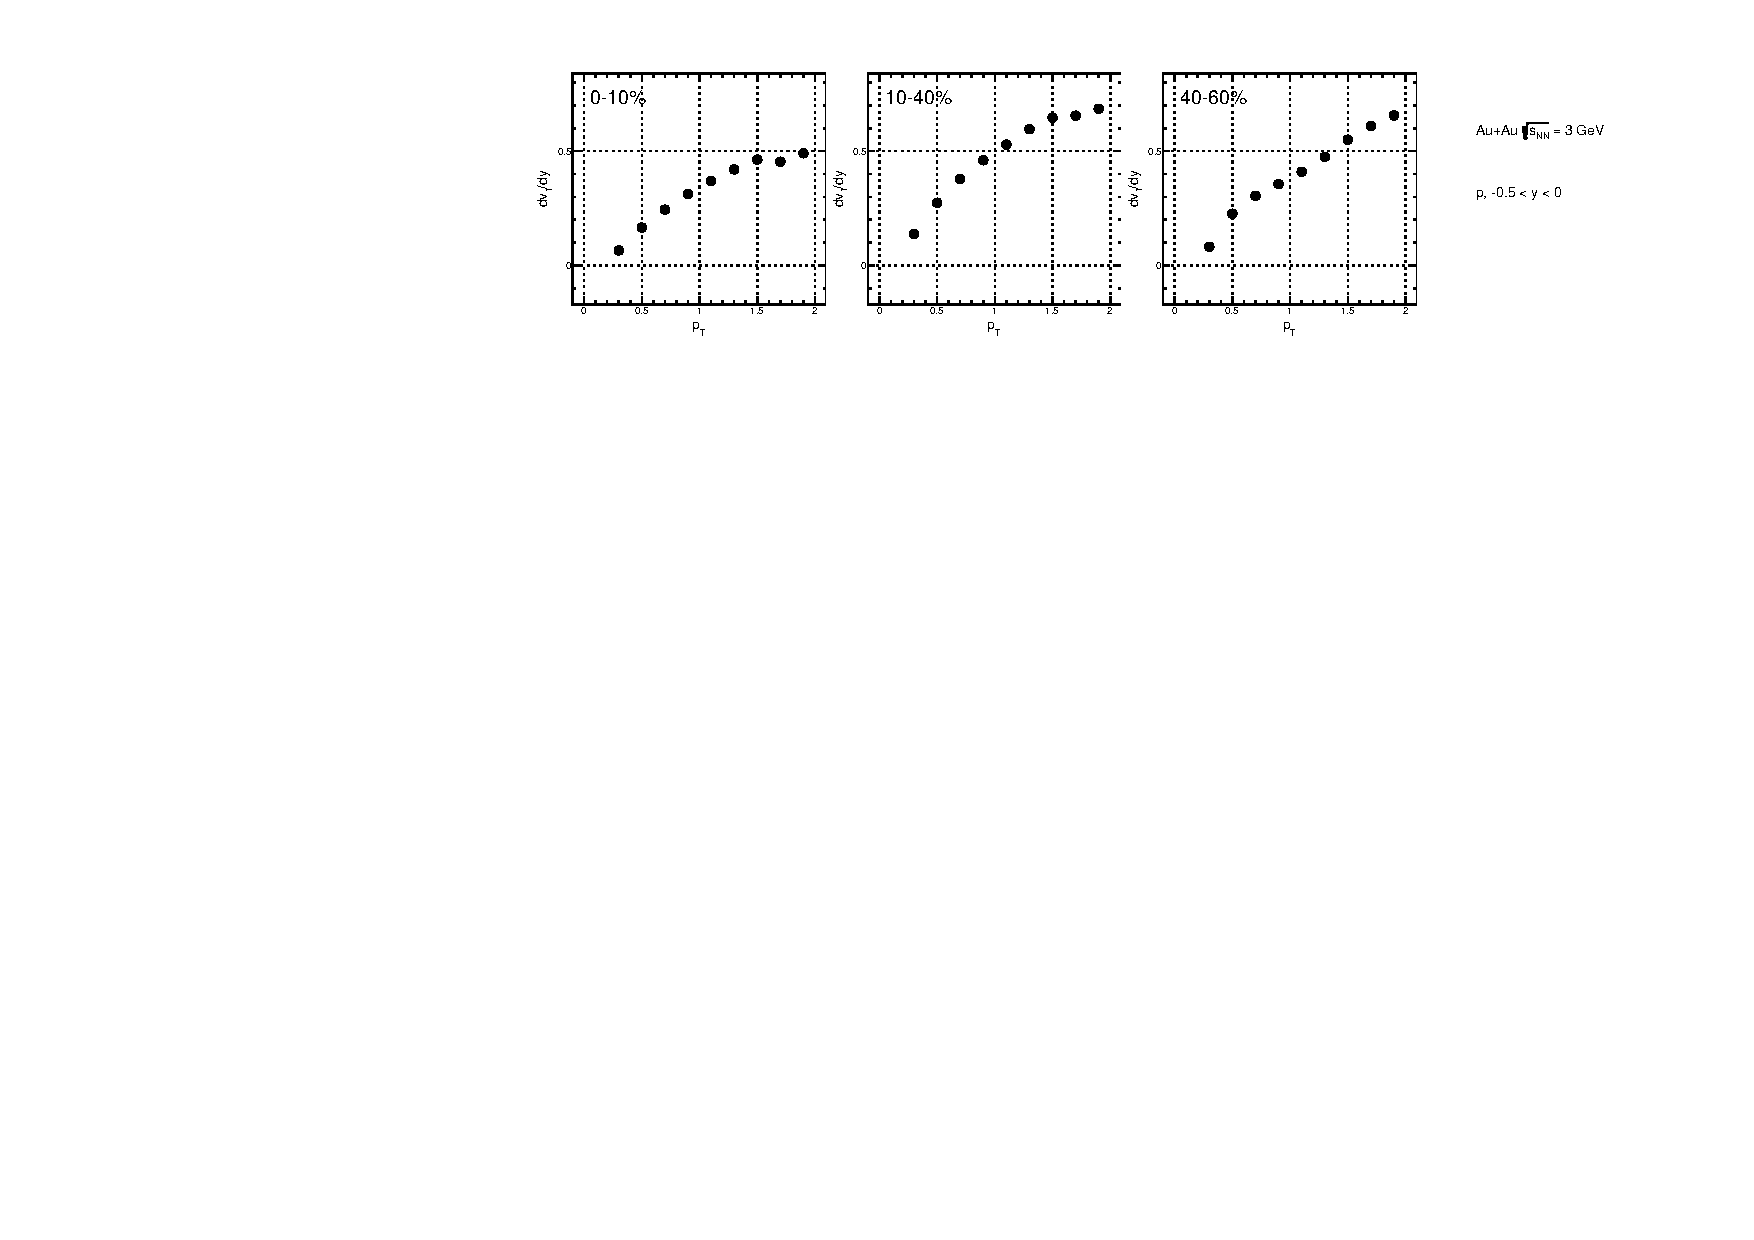
\includegraphics[scale=0.7]{FXT3gev/chapter3/fig/v1ptpikp/prp_dv1pt_widecent.pdf}
\caption{protons' $dv_{1}/dy$ as a function of transverse momentum ($p_{T}$) in Au+Au collisions at $\sqrt{s_{NN}}$ = 3 GeV in 0-10\%, 10-40\% and 40-60\% centrality bins.}
\label{proton_dv1pt_widecent}
\end{figure}



\clearpage
\subsection{$v_{2}$ results for $\pi, K, p$}
In this chapter, we will show the $v_{2}$ as a function of $p_{T}$ and rapidity(y) in fine centrality bins for $\pi^{\pm}, K^{\pm}$ and proton. It is expected to have a negative $v_{2}$ value at mid-rapidity region based on world data due to the "squeeze-out" effect when the center of mass energy is below 4 GeV. This is because at such low energy, the passage time of projectile and target spectators is comparable or larger than the expansion time QGP mediums, thus the spectators will shadow or squeeze out the medium expansion in the impact parameter direction, which will results in the out-of plane $v_{2}$, the negative $v_{2}$ value.

\subsubsection{pions $v_{2}$ as a function of $p_{T}$ and rapidity}
In this chapter, we will show the results of pions' $v_{2}$ as a function of $p_{T}$ and rapidity(y).
Figure \ref{pion_v2y_cent} shows pion $v_{2}$ as a function of y for different centrality bins from 0-5\% to 50-60\%. The $p_{T}$ range is [0.2, 1.6] GeV/c. As we can see, we have observed the negative pion $v_{2}$ value at mid-rapidity region, and it has weak rapidity dependence for both $\pi^{+}$ and $\pi^{-}$. Which we do see the difference between $\pi^{+}$ and $\pi^{-}$ $v_{2}$, $\pi^{-}$ $v_{2}$ is a little larger than $\pi^{+}$ $v_{2}$. In the BES-I flow results, we also see the difference between $\pi^{+}$ and $\pi^{-}$ $v_{2}$, which has been interpreted by the isospin effect or mean-filed potential effect. Figure \ref{pion_v2y_widecent} shows the pions' $v_{2}$ vs. y in wider centrality bin.

\begin{figure}[h]
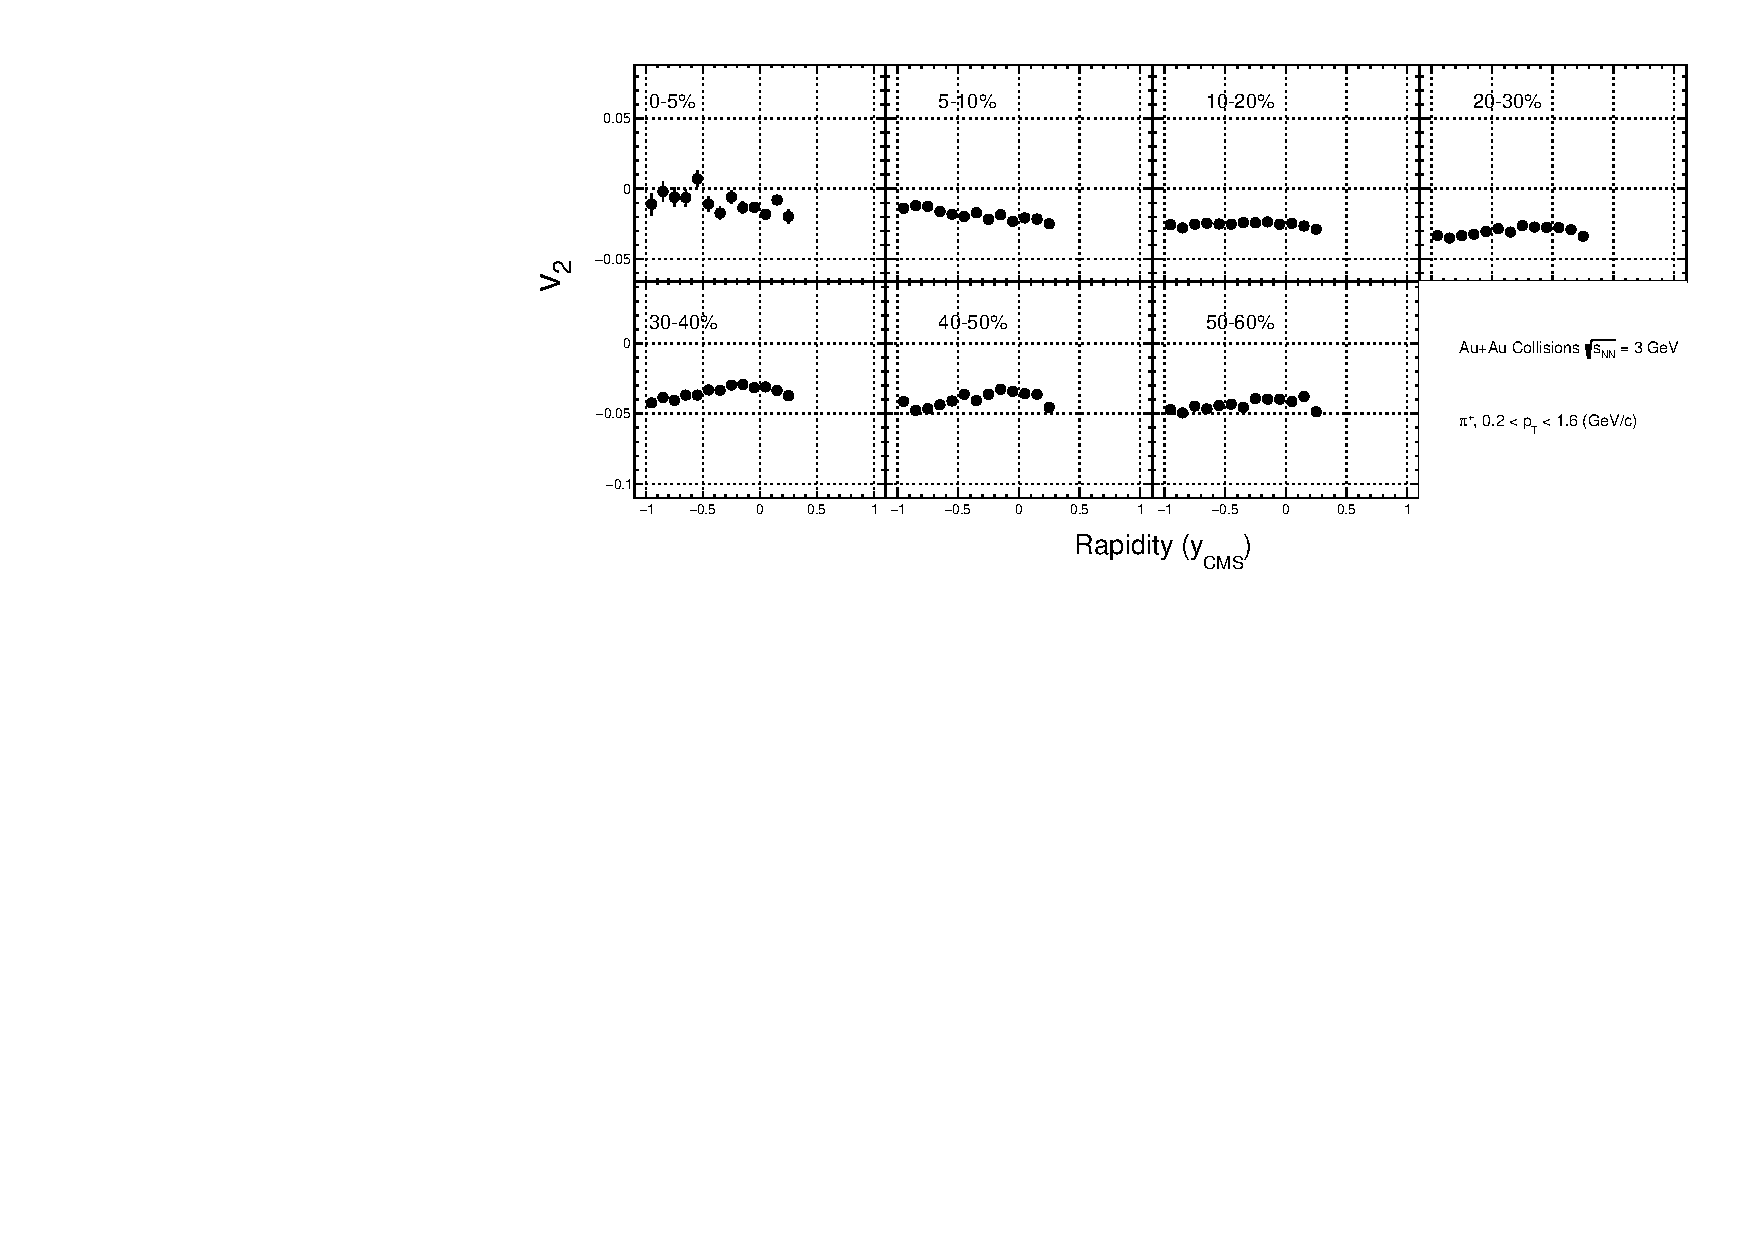
\includegraphics[scale=0.4]{chapter3/fig/v2ypikp/v2y_cent_pionp.pdf}
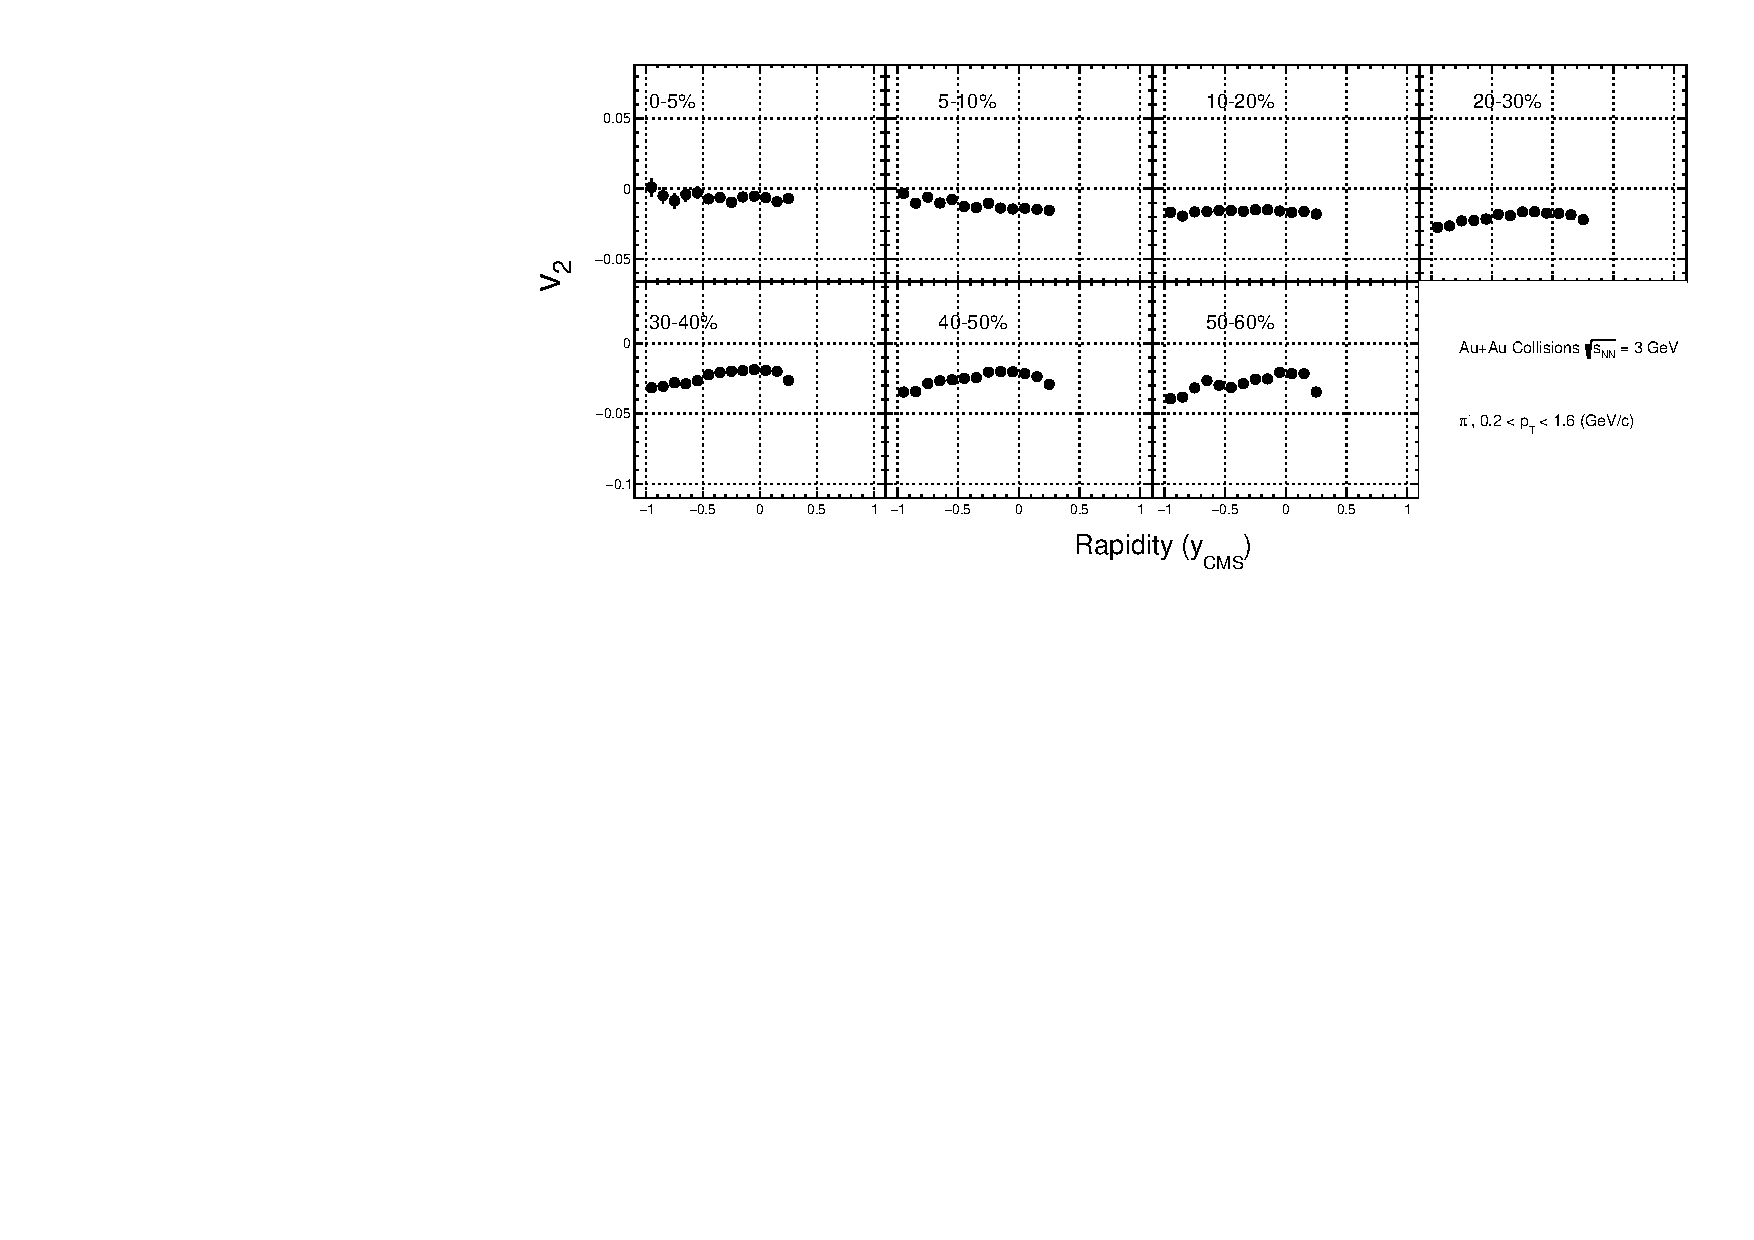
\includegraphics[scale=0.4]{chapter3/fig/v2ypikp/v2y_cent_pionm.pdf}
\caption{\label{pion_v2y_cent} $v_{2}$ as a function of rapidity(y) in different centrality bins for $\pi^{+}$ and $\pi^{-}$ in Au+Au collisions at $\sqrt{s_{NN}}$ = 3 GeV.}
\end{figure}

\begin{figure}[h]
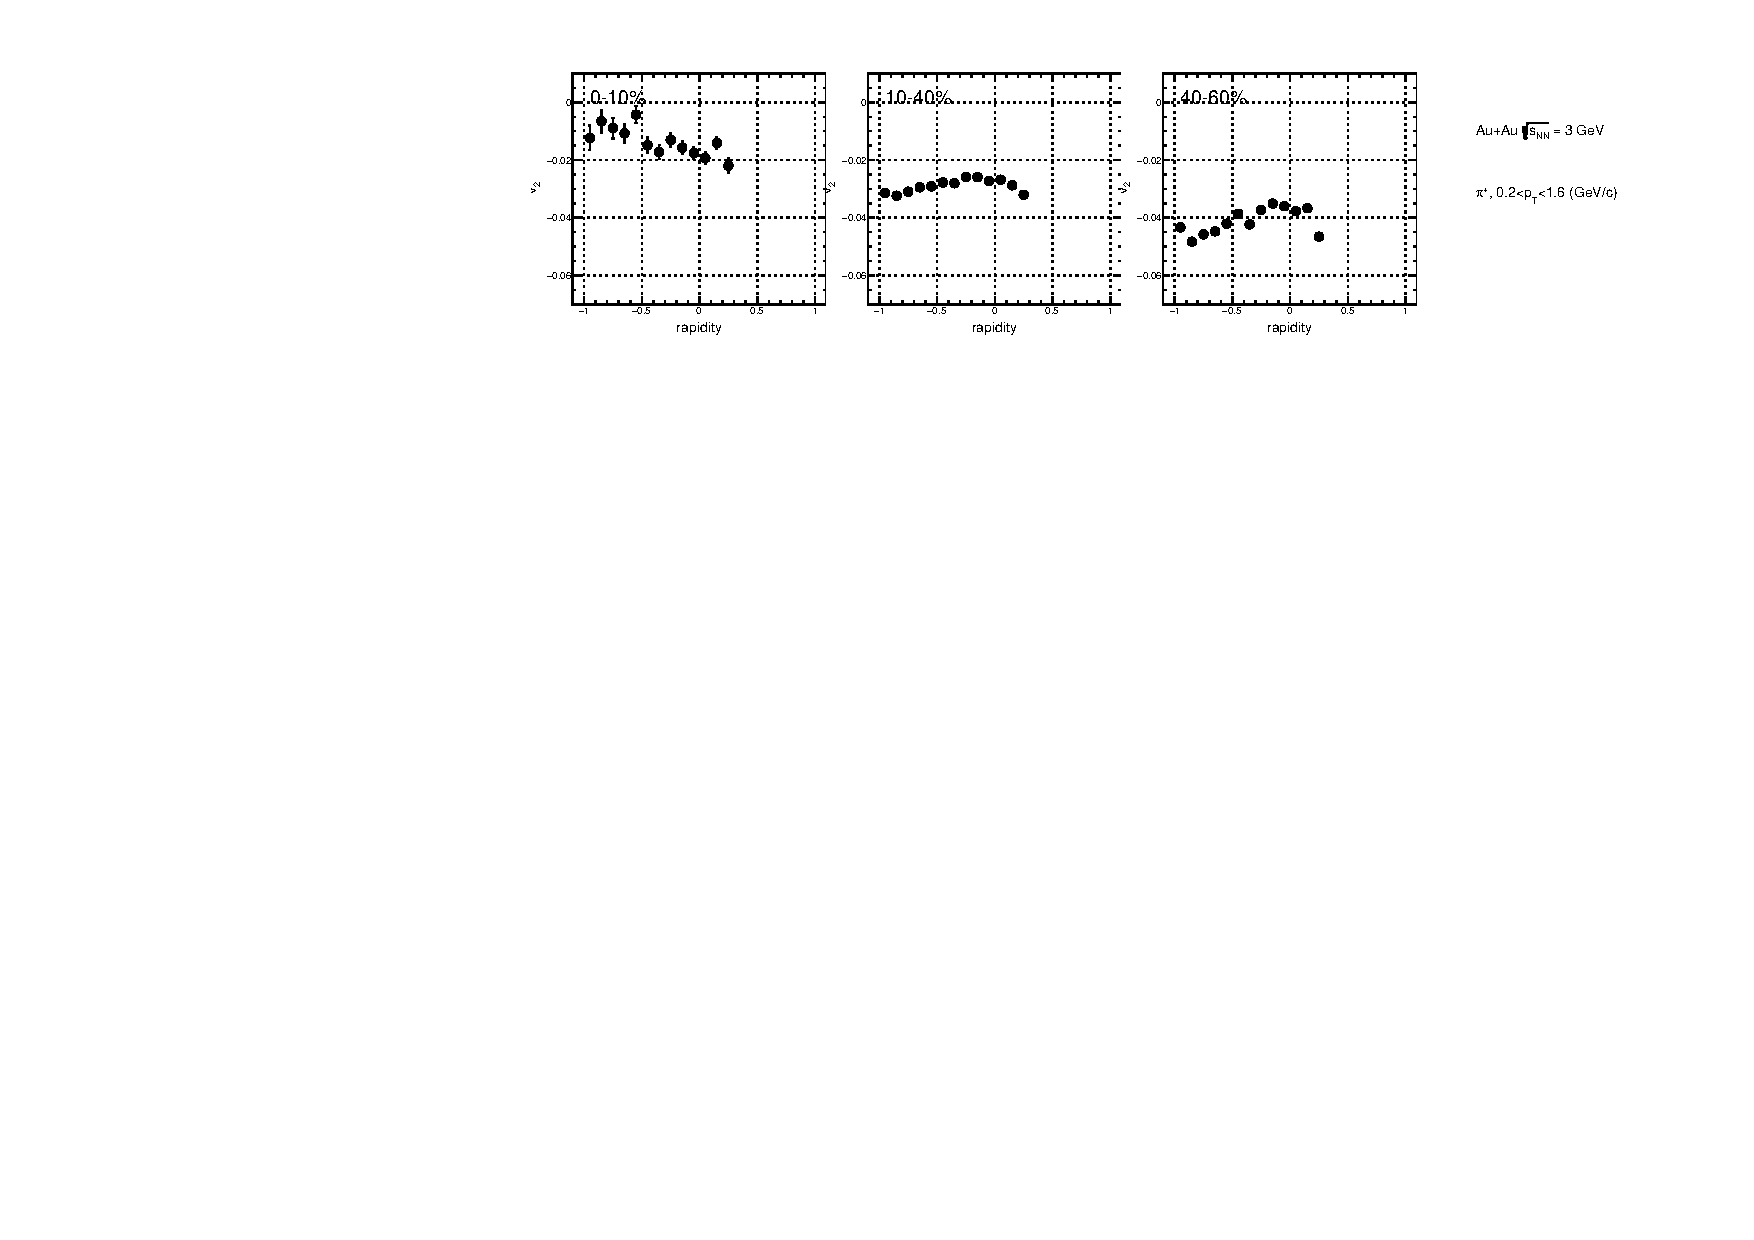
\includegraphics[scale=0.6]{chapter3/fig/v2ypikp/pionp_v2y_wide_cent.pdf}
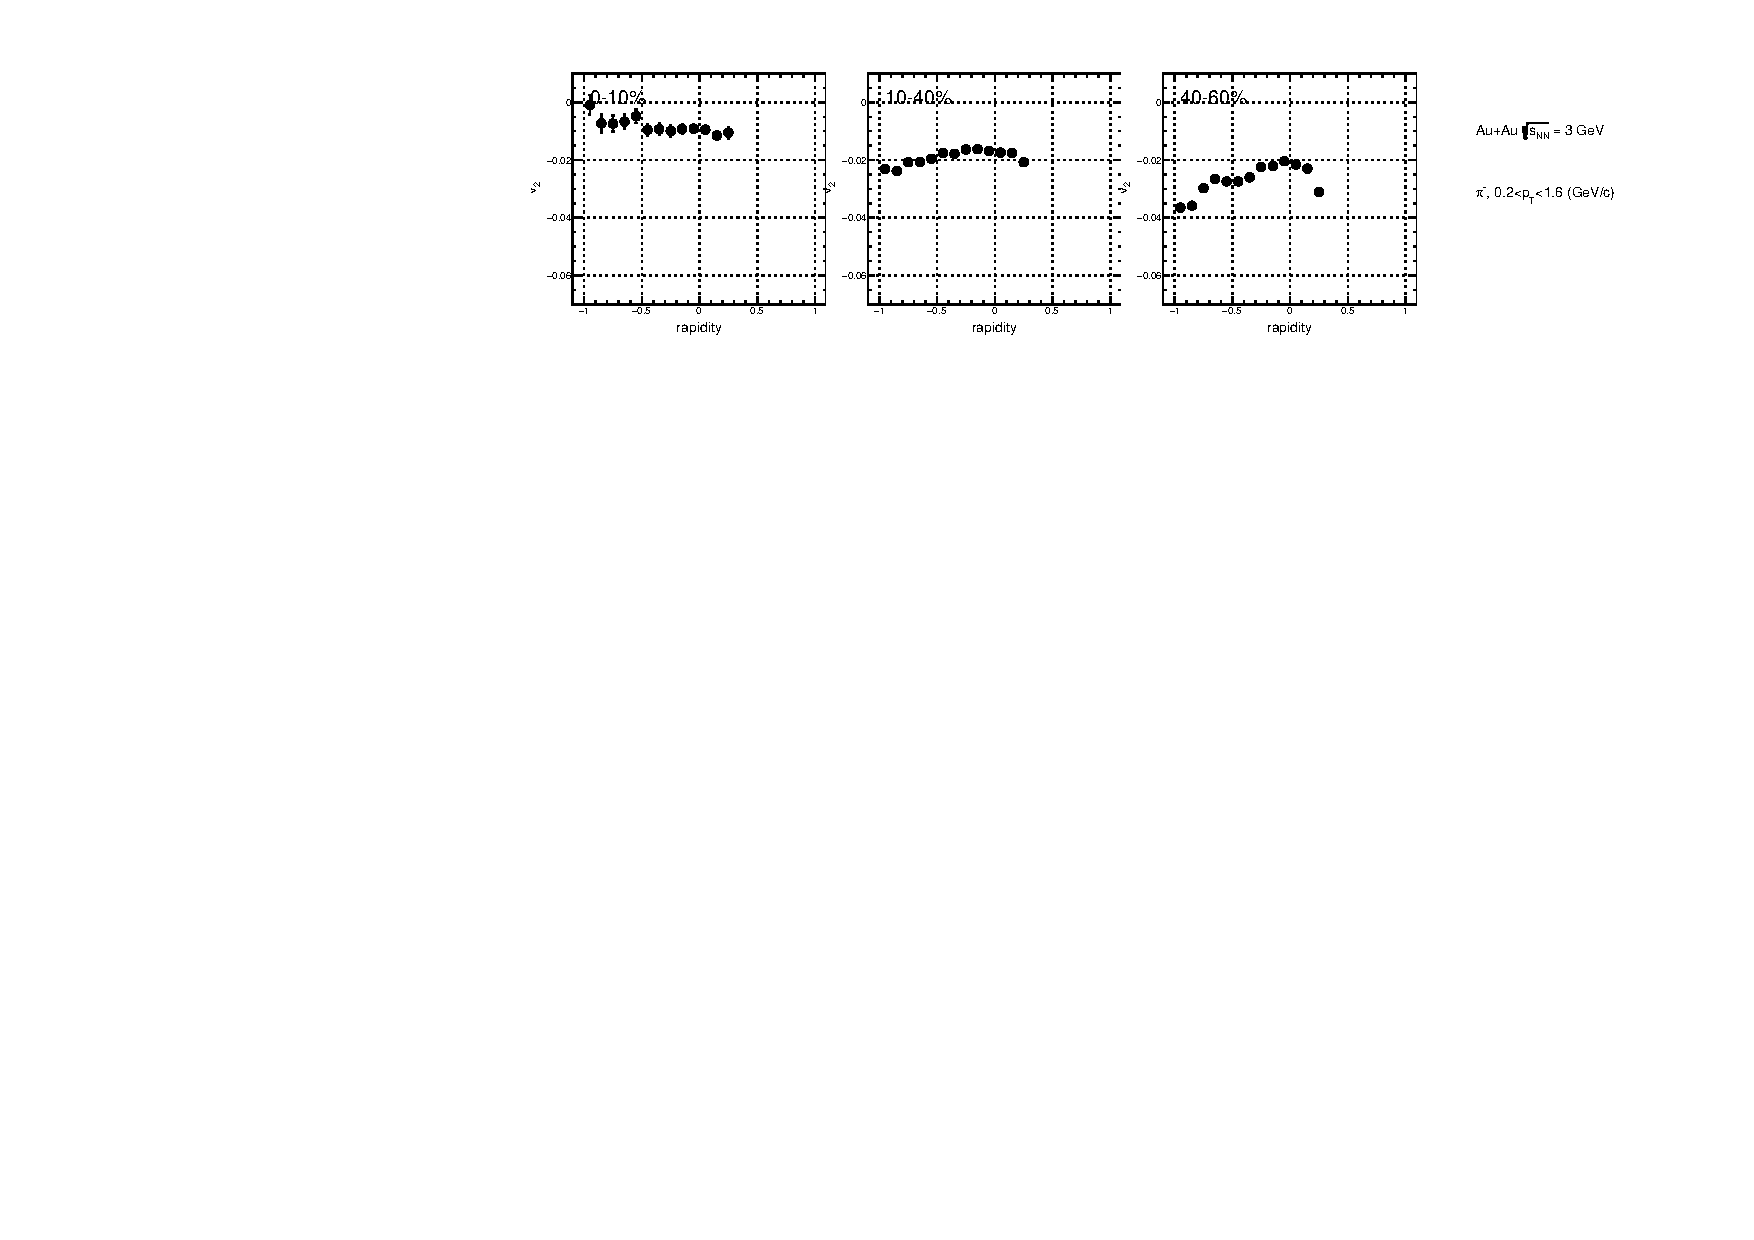
\includegraphics[scale=0.6]{chapter3/fig/v2ypikp/pionm_v2y_wide_cent.pdf}
\caption{\label{pion_v2y_widecent} $v_{2}$ as a function of rapidity(y) in different centrality bins for $\pi^{+}$ and $\pi^{-}$ in Au+Au collisions at $\sqrt{s_{NN}}$ = 3 GeV in 0-10\%, 10-40\%, 40-60\% centrality bins.}
\end{figure}

We also study the $p_{T}$ dependence for pions' $v_{2}$ in the figure \ref{pion_v2pt_cent}, as we can see, pions' $v_{2}$ is decreasing with $p_{T}$ increasing. Figure \ref{pion_v2pt_widecent} shows these results in wider centrality bins 0-10\%, 10-40\%, 40-60\%. 


\begin{figure}[h]
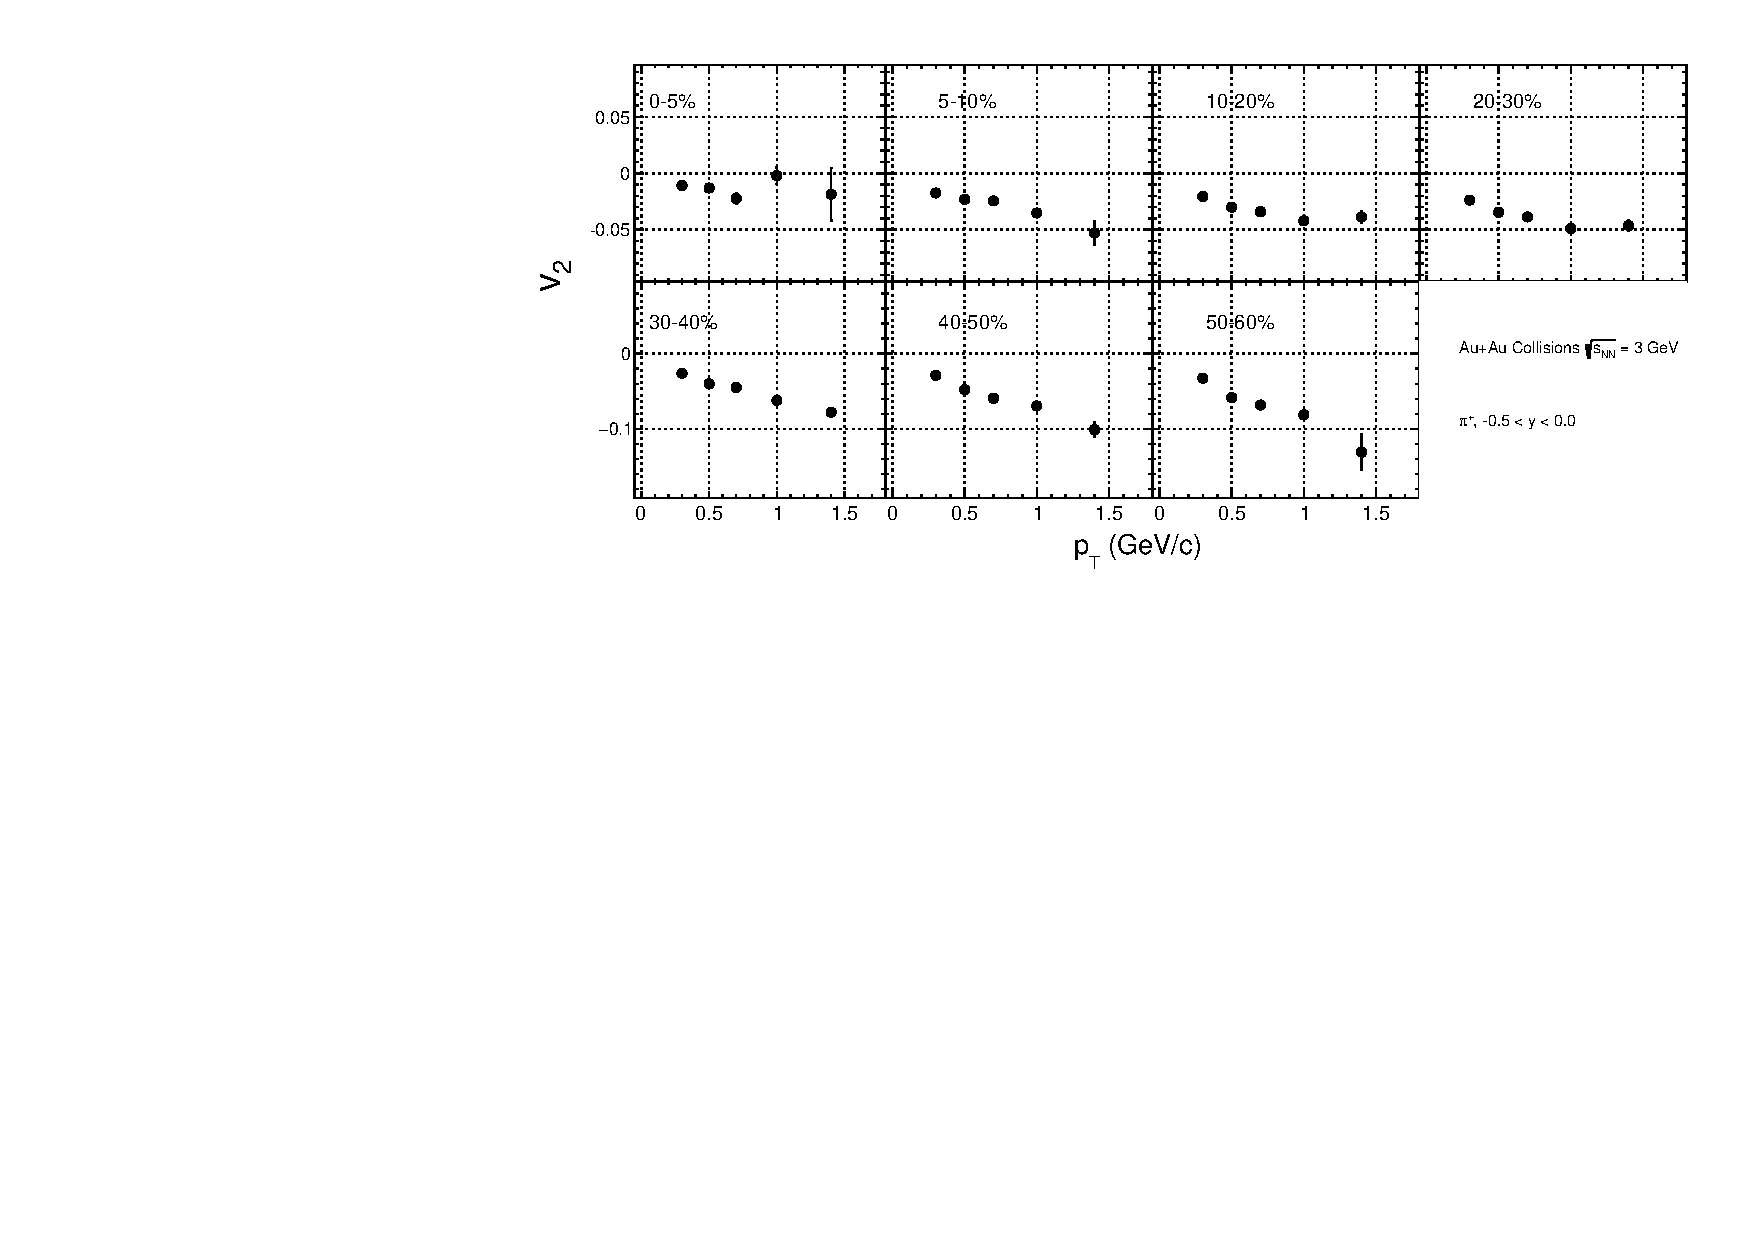
\includegraphics[scale=0.4]{chapter3/fig/v2ptpikp/v2pt_cent_pionp.pdf}
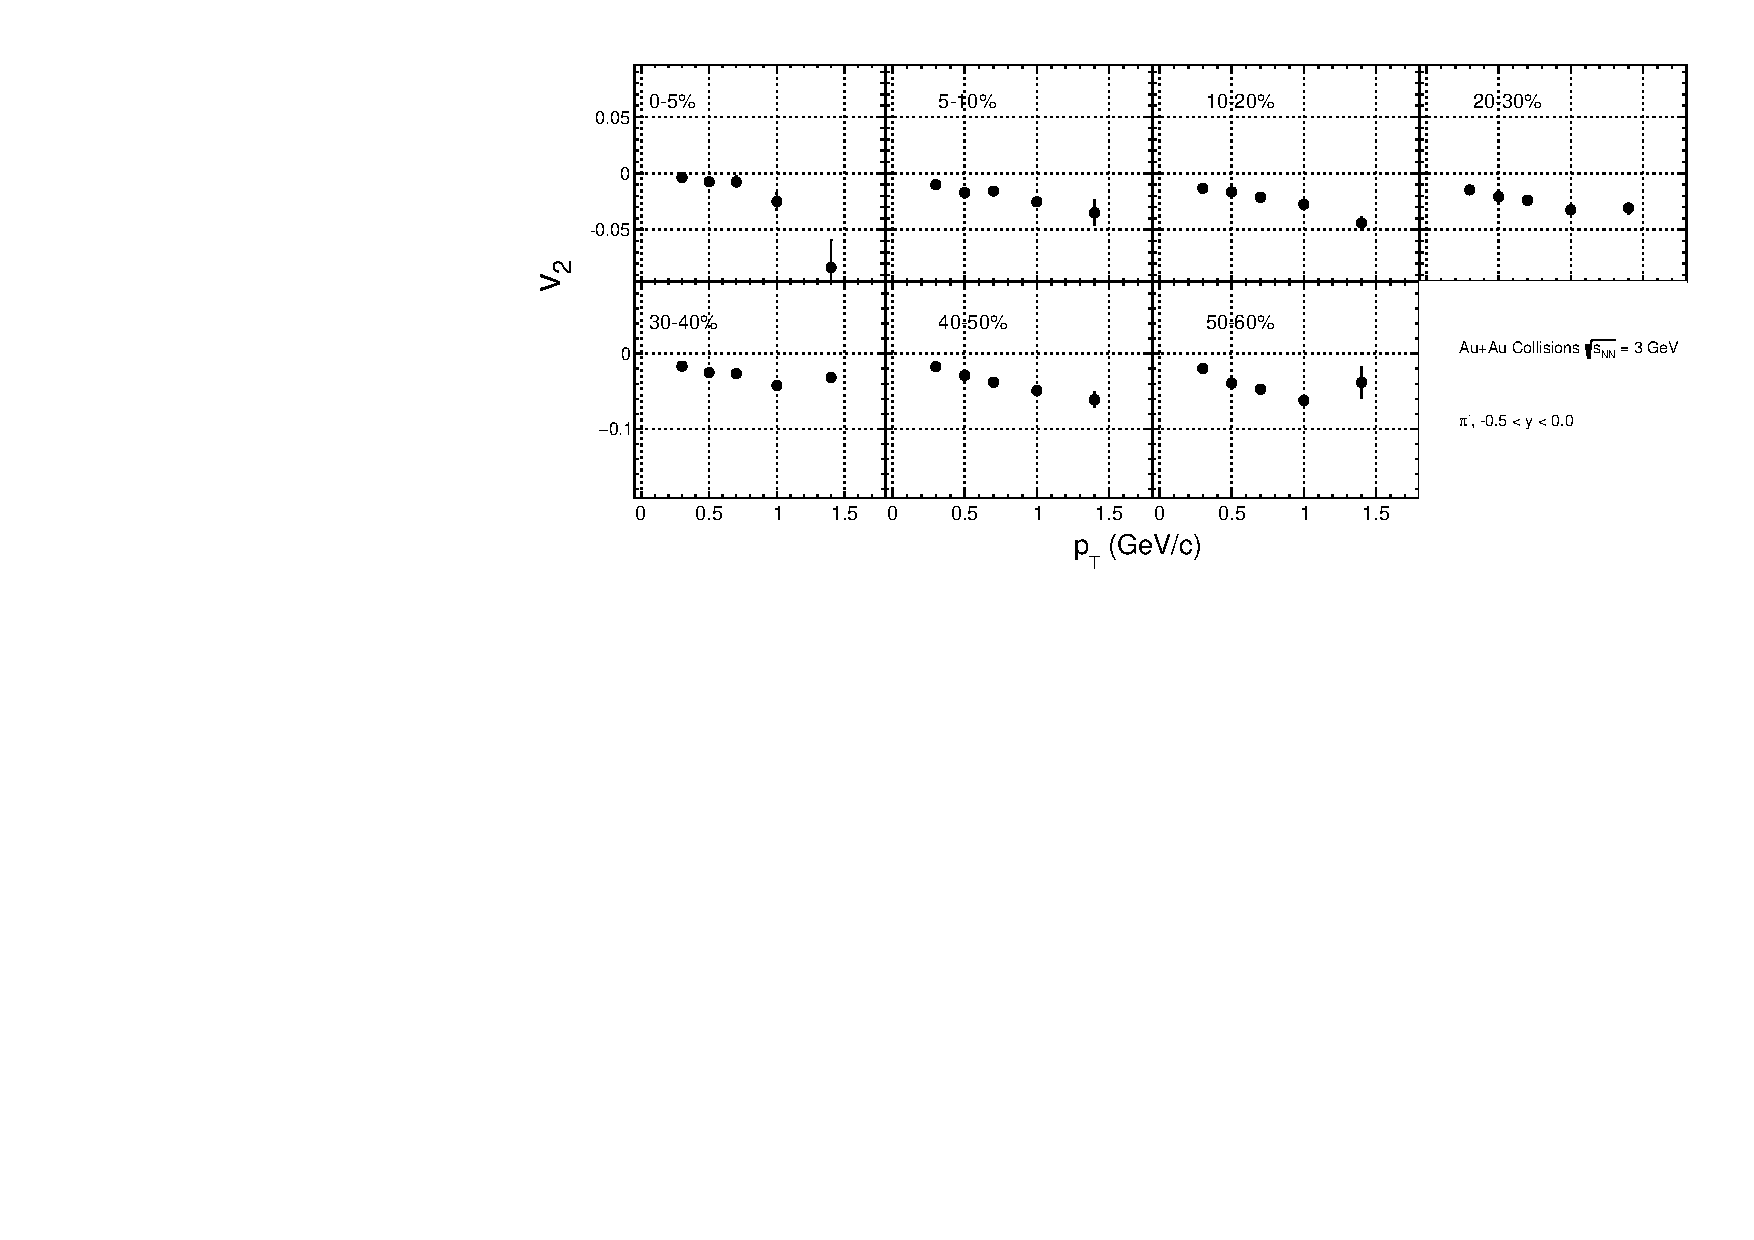
\includegraphics[scale=0.4]{chapter3/fig/v2ptpikp/v2pt_cent_pionm.pdf}
\caption{$v_{2}$ as a function of $p_{T}$ in different centrality bins for $\pi^{+}$ and $\pi^{-}$ in Au+Au collisions at $\sqrt{s_{NN}}$ = 3 GeV.}
\label{pion_v2pt_cent}
\end{figure}

\begin{figure}[h]
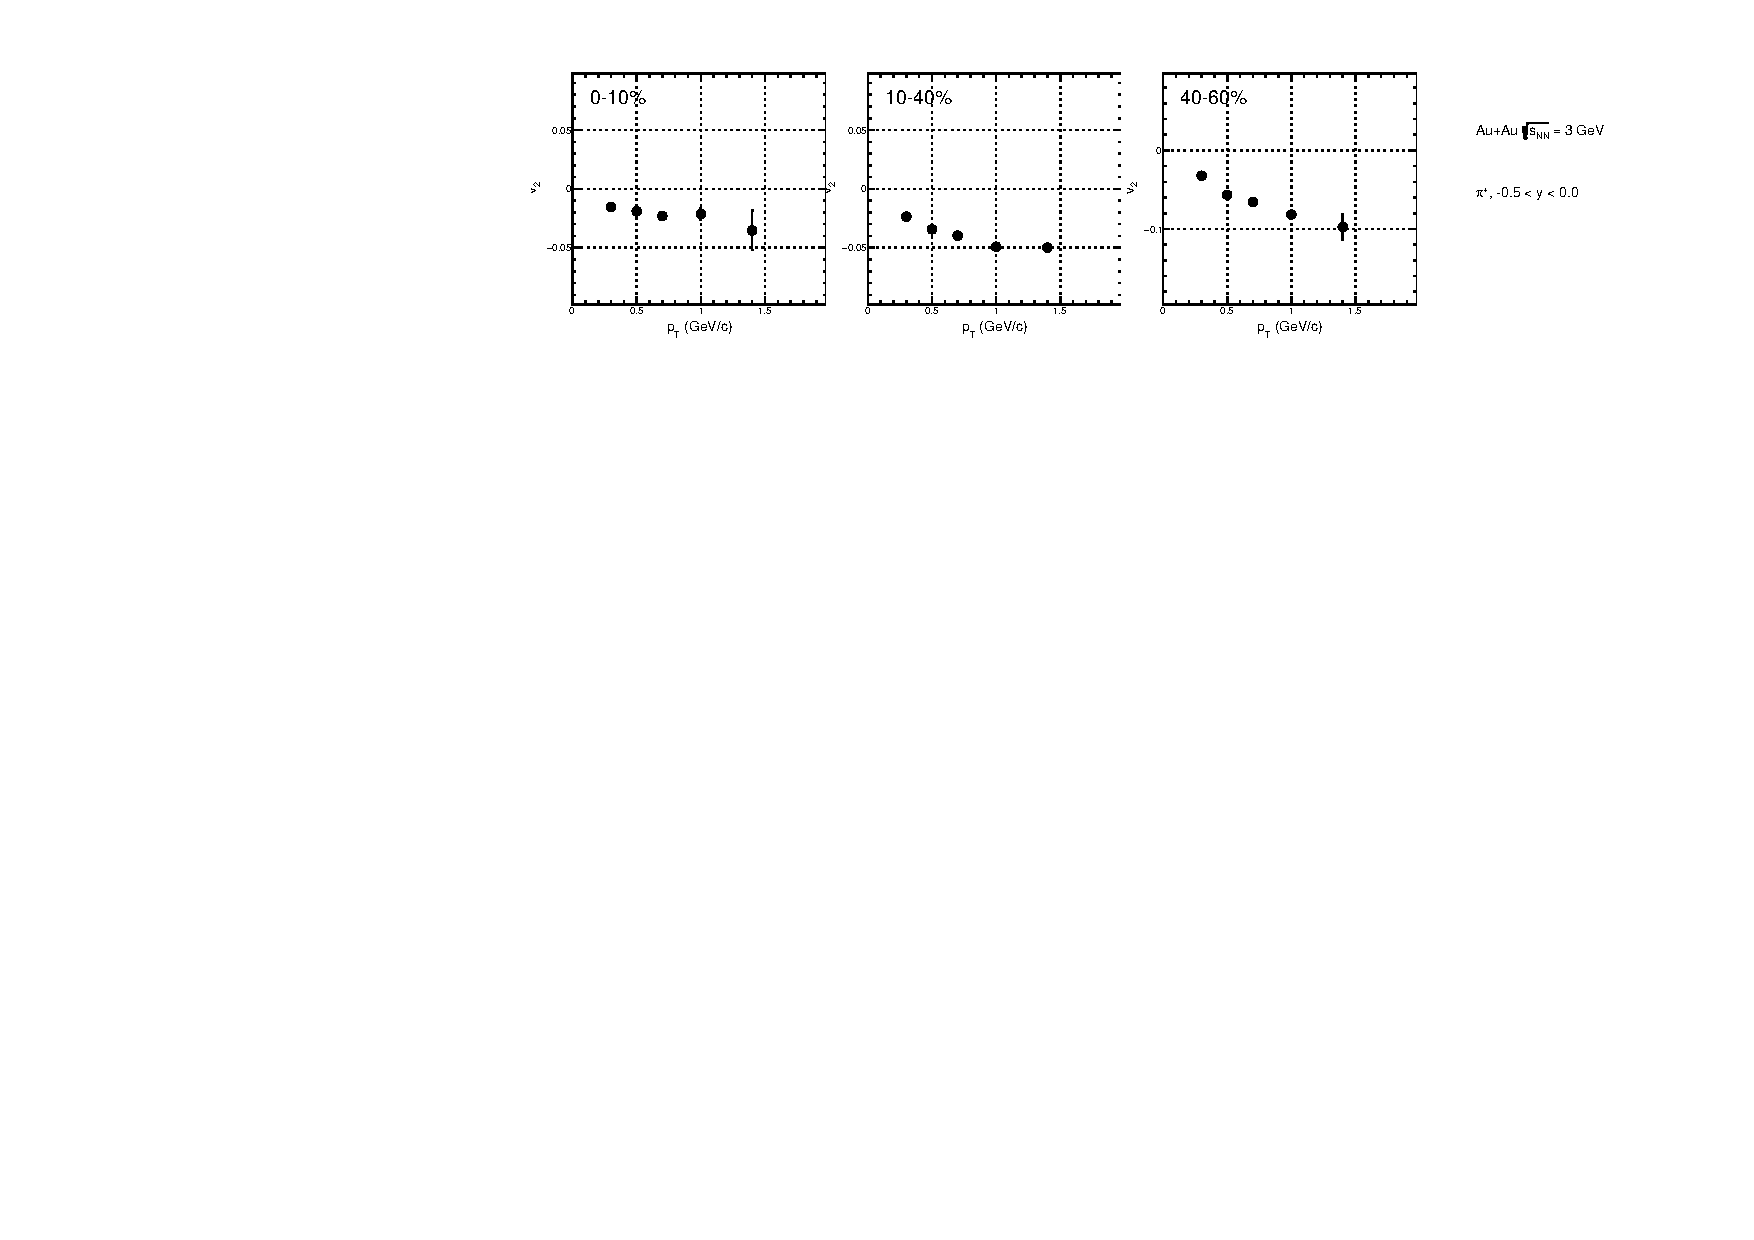
\includegraphics[scale=0.5]{chapter3/fig/v2ptpikp/pionp_v2pt_wide_cent.pdf}
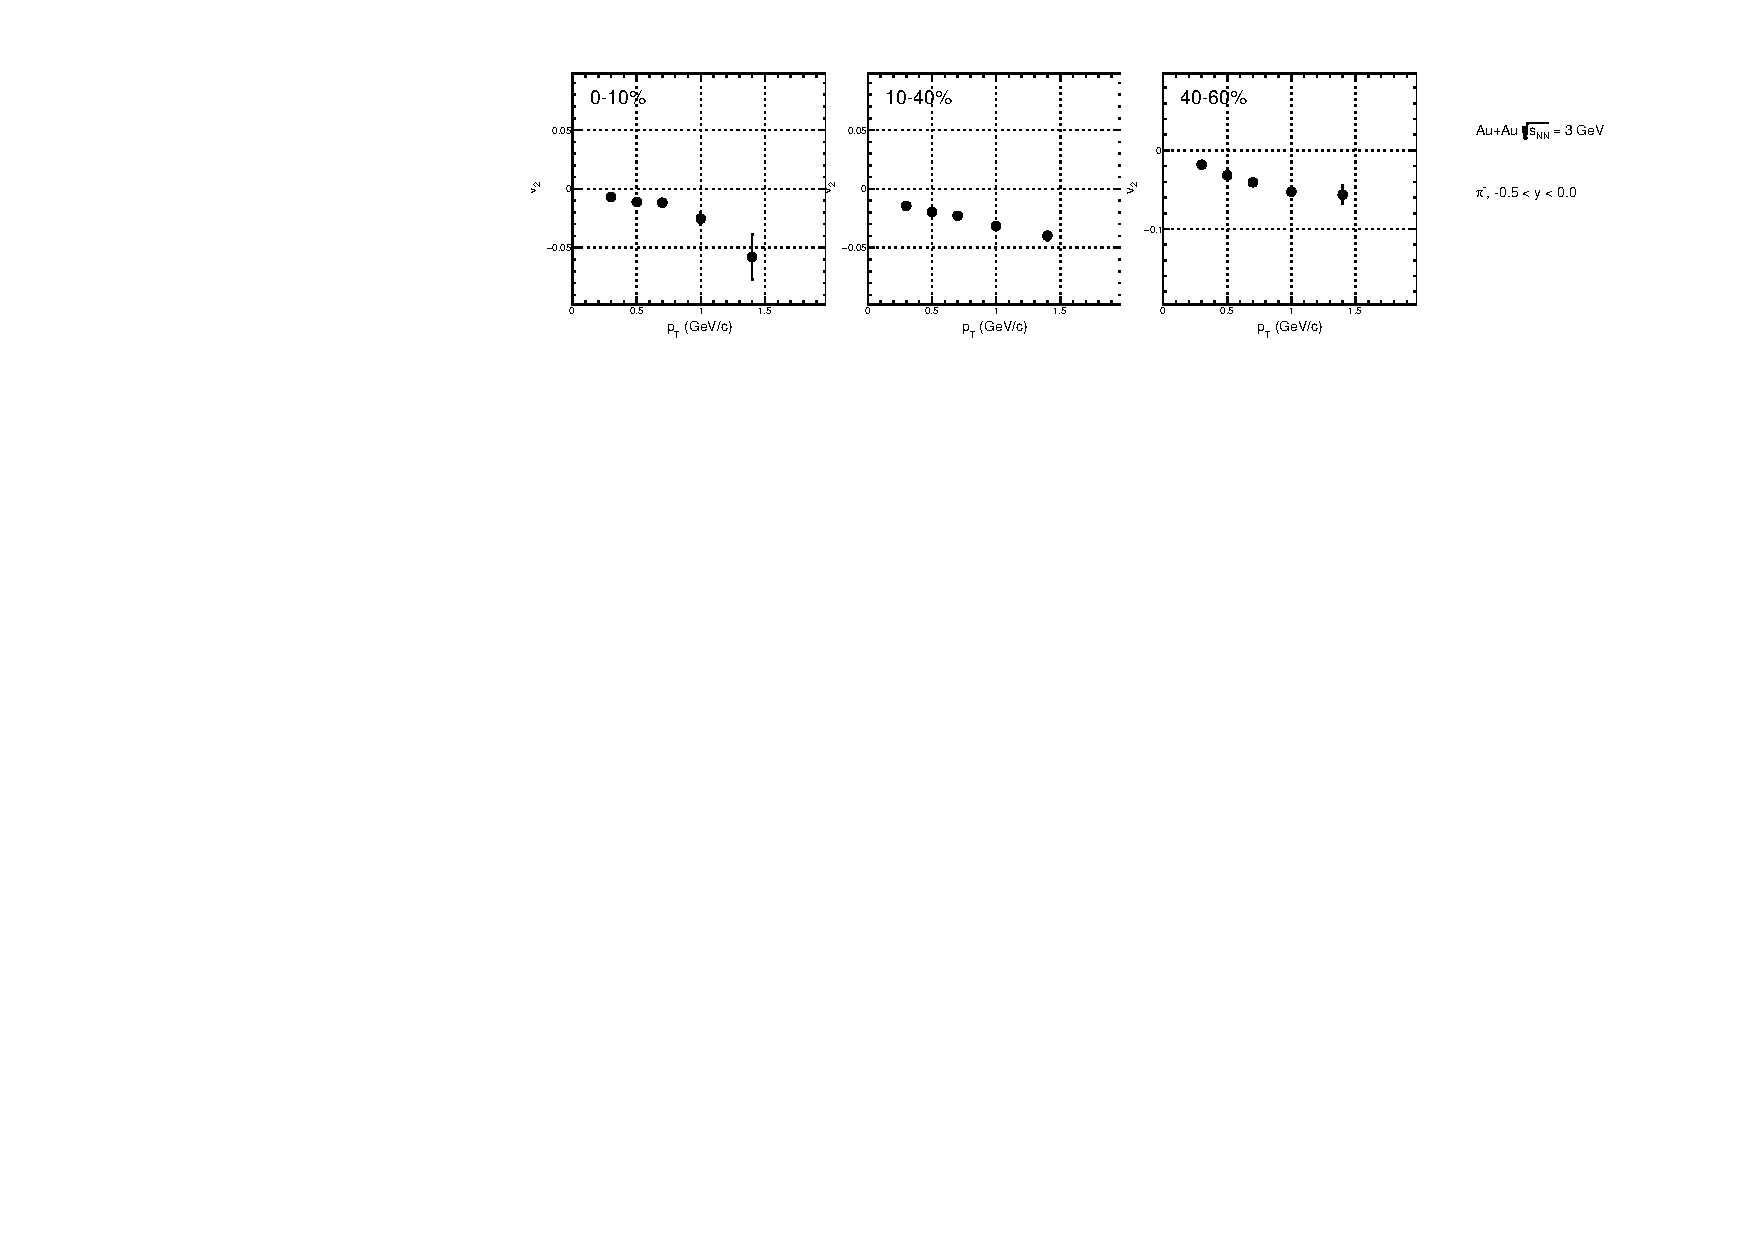
\includegraphics[scale=0.5]{chapter3/fig/v2ptpikp/pionm_v2pt_wide_cent.pdf}
\caption{$v_{2}$ as a function of $p_{T}$ in different centrality bins for $\pi^{+}$ and $\pi^{-}$ in Au+Au collisions at $\sqrt{s_{NN}}$ = 3 GeV in 0-10\%, 10-40\%, 40-60\% centrality bins.}
\label{pion_v2pt_widecent}
\end{figure}



\clearpage


\subsubsection{kaons $v_{2}$ as a function of $p_{T}$ and rapidity}
In this chapter, we will show the results of kaons' $v_{2}$ as a function of $p_{T}$ and rapidity(y).
Figure \ref{kaon_v2y_cent} shows kaon $v_{2}$ as a function of y for different centrality bins from 0-5\% to 50-60\%. The $p_{T}$ range is [0.4, 1.6] GeV/c. Figure \ref{kaon_v2y_widecent} shows the kaons' $v_{2}$ vs. y in wider centrality bin. $K^{+}$ and $K^{-}$ $v_{2}$ are consistent within error bar.



\begin{figure}[h]
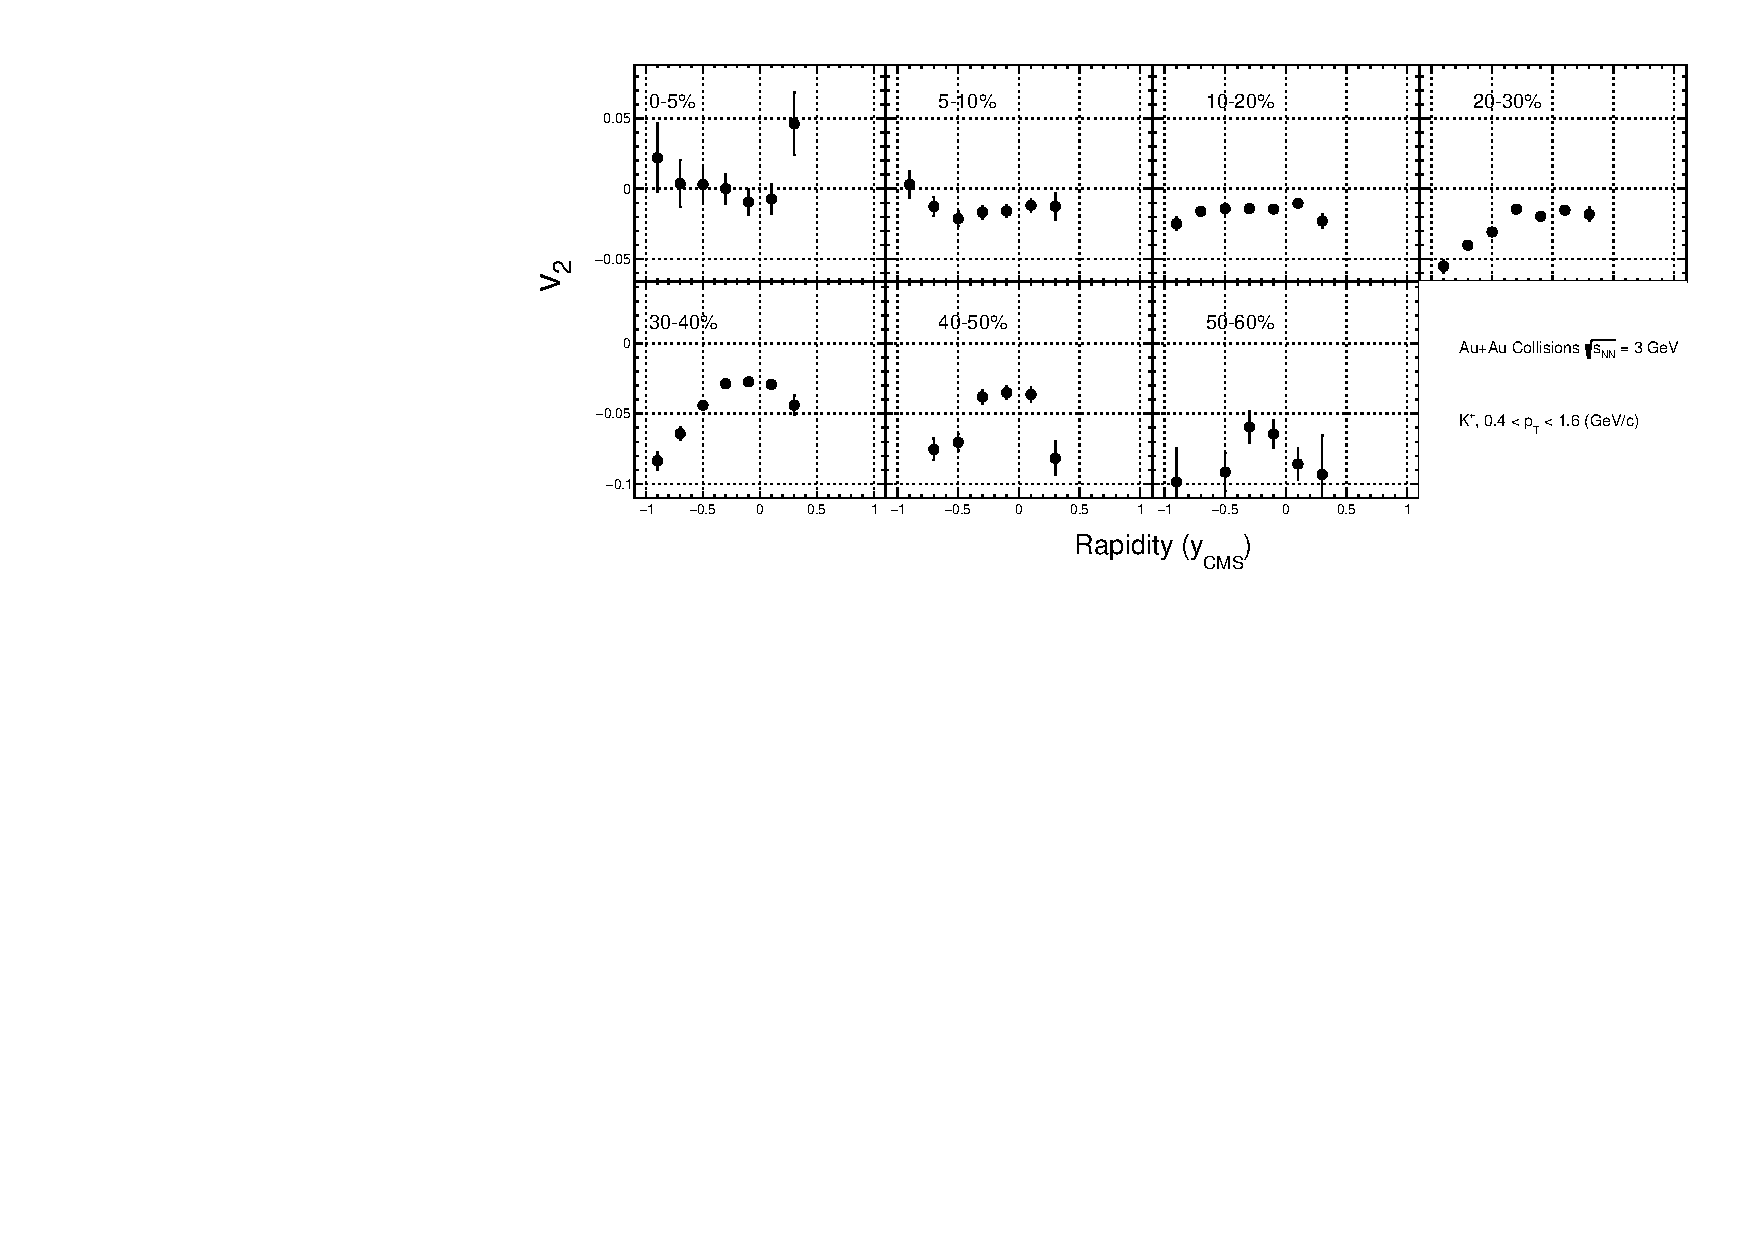
\includegraphics[scale=0.4]{chapter3/fig/v2ypikp/v2y_cent_kaonp.pdf}
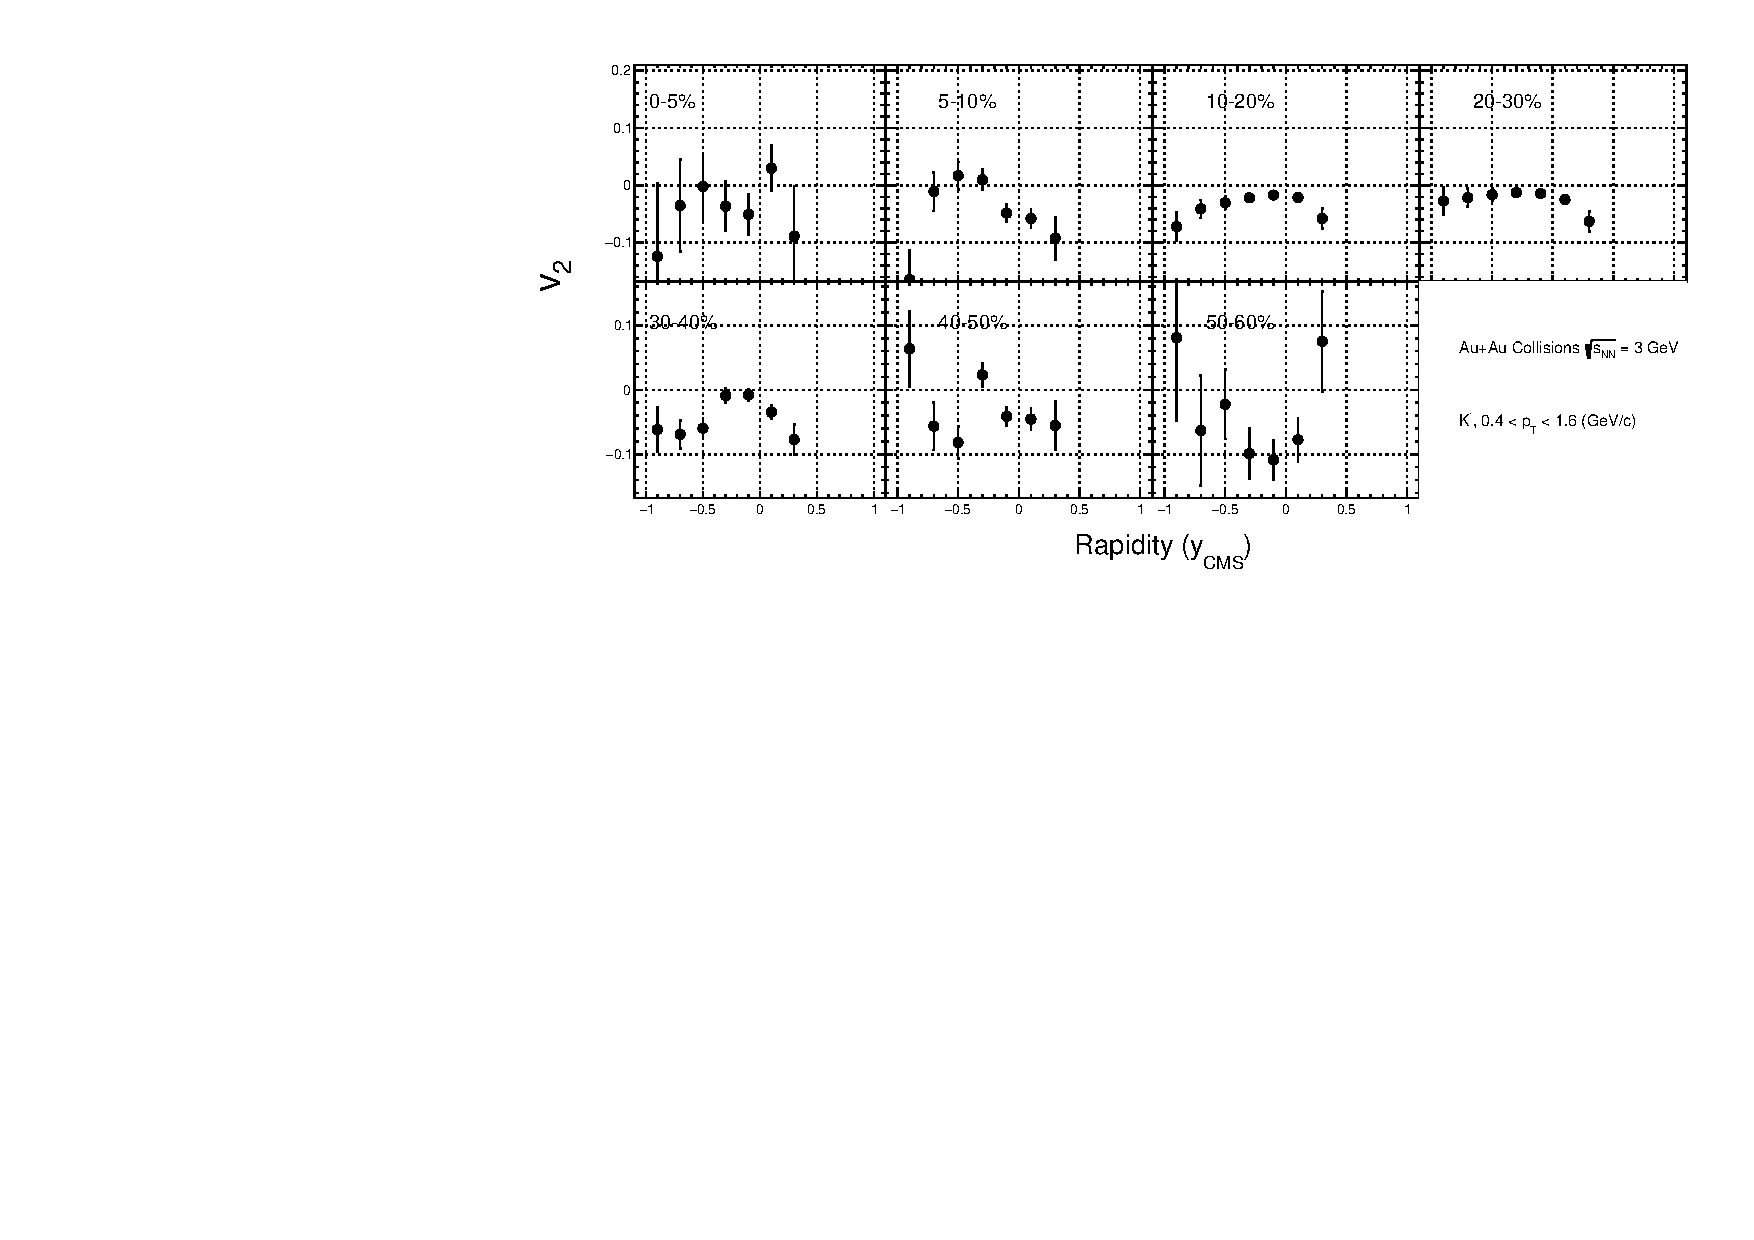
\includegraphics[scale=0.4]{chapter3/fig/v2ypikp/v2y_cent_kaonm.pdf}
\caption{$v_{2}$ as a function of rapidity(y) in different centrality bins for $K^{+}$ and $K^{-}$ in Au+Au collisions at $\sqrt{s_{NN}}$ = 3 GeV.}
\label{kaon_v2y_cent}
\end{figure}

\begin{figure}[h]
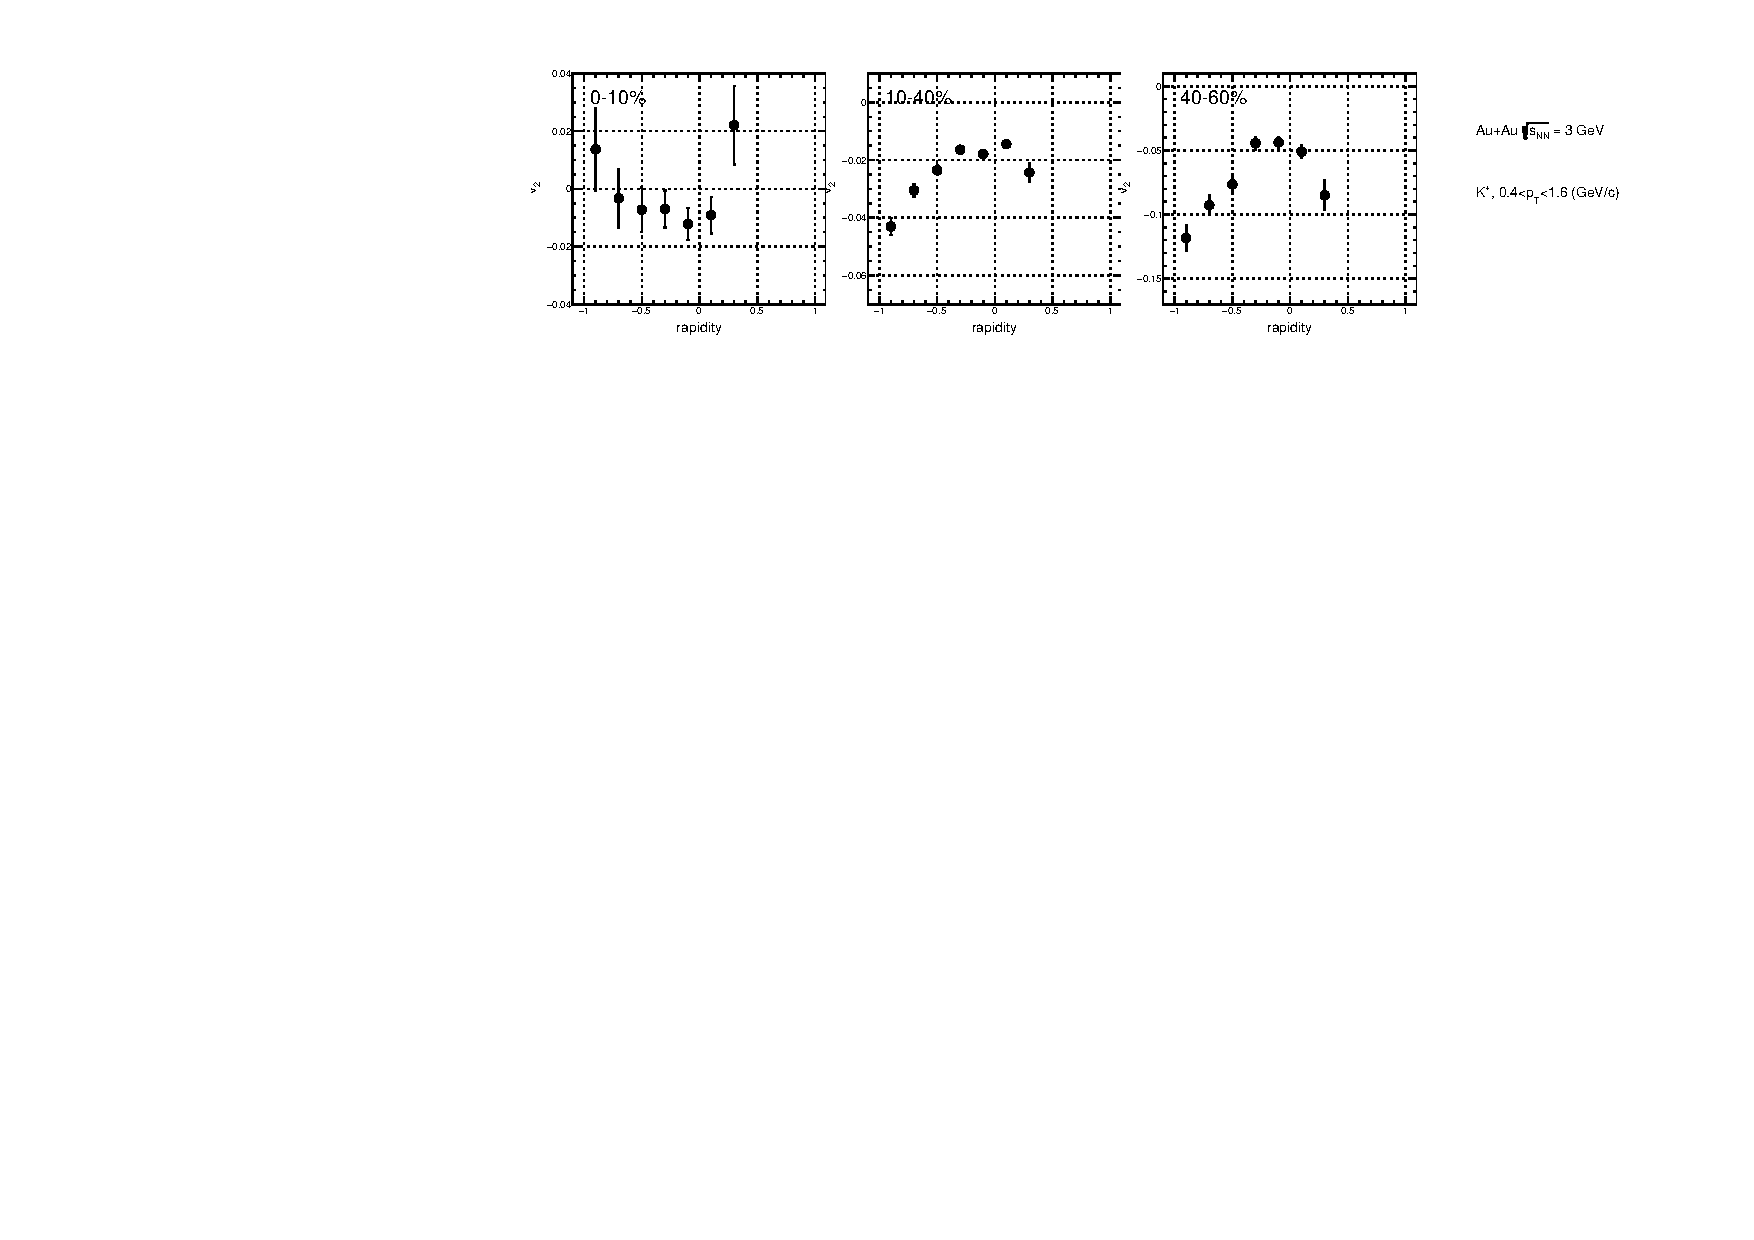
\includegraphics[scale=0.6]{chapter3/fig/v2ypikp/kaonp_v2y_wide_cent.pdf}
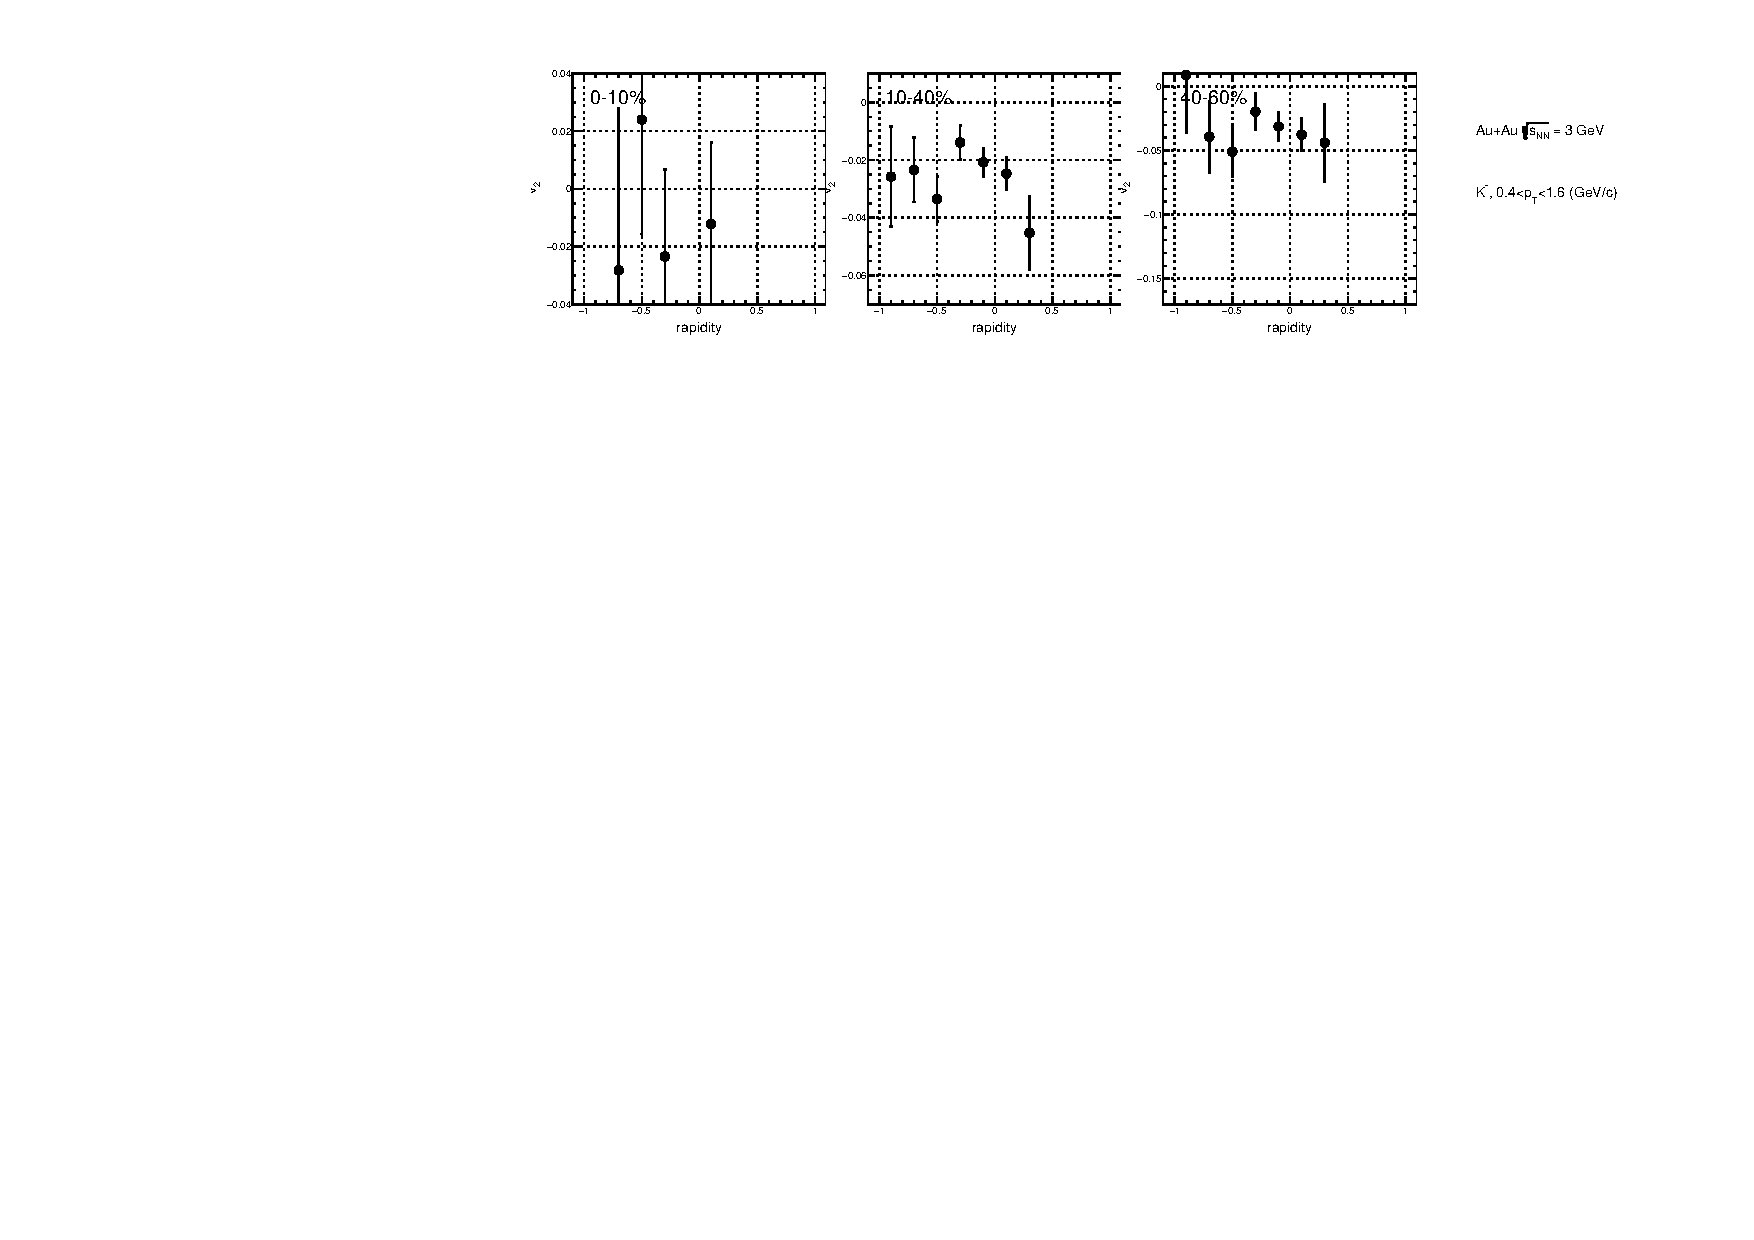
\includegraphics[scale=0.6]{chapter3/fig/v2ypikp/kaonm_v2y_wide_cent.pdf}
\caption{$v_{2}$ as a function of rapidity(y) in different centrality bins for $K^{+}$ and $K^{-}$ in Au+Au collisions at $\sqrt{s_{NN}}$ = 3 GeV in 0-10\%, 10-40\%, 40-60\% centrality bins.}
\label{kaon_v2y_widecent}
\end{figure}

We also study the $p_{T}$ dependence for kaons' $v_{2}$ in the figure \ref{kaon_v2pt_cent}, as we can see, kaons' $v_{2}$ is decreasing with $p_{T}$ increasing. Figure \ref{kaon_v2pt_widecent} shows these results in wider centrality bins 0-10\%, 10-40\%, 40-60\%. 


\begin{figure}[h]
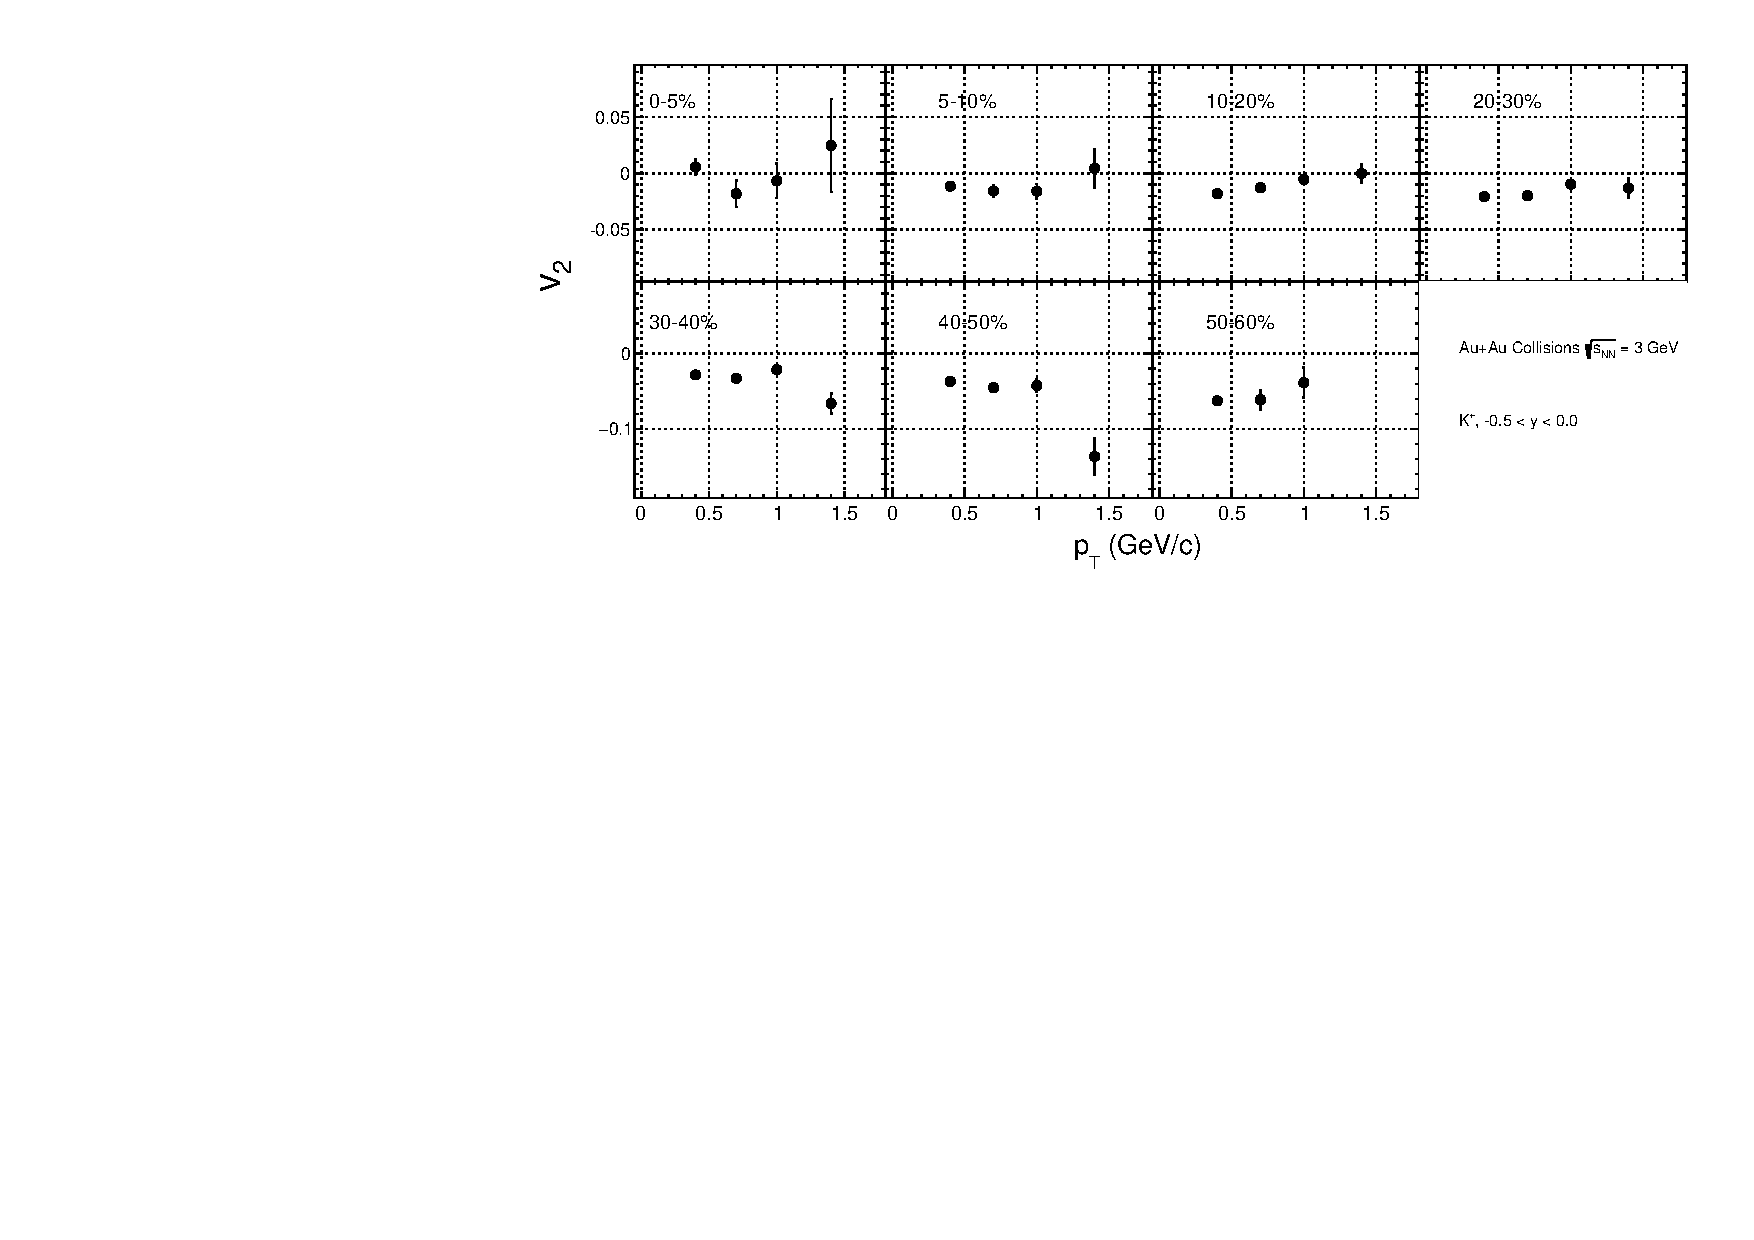
\includegraphics[scale=0.5]{chapter3/fig/v2ptpikp/v2pt_cent_kaonp.pdf}
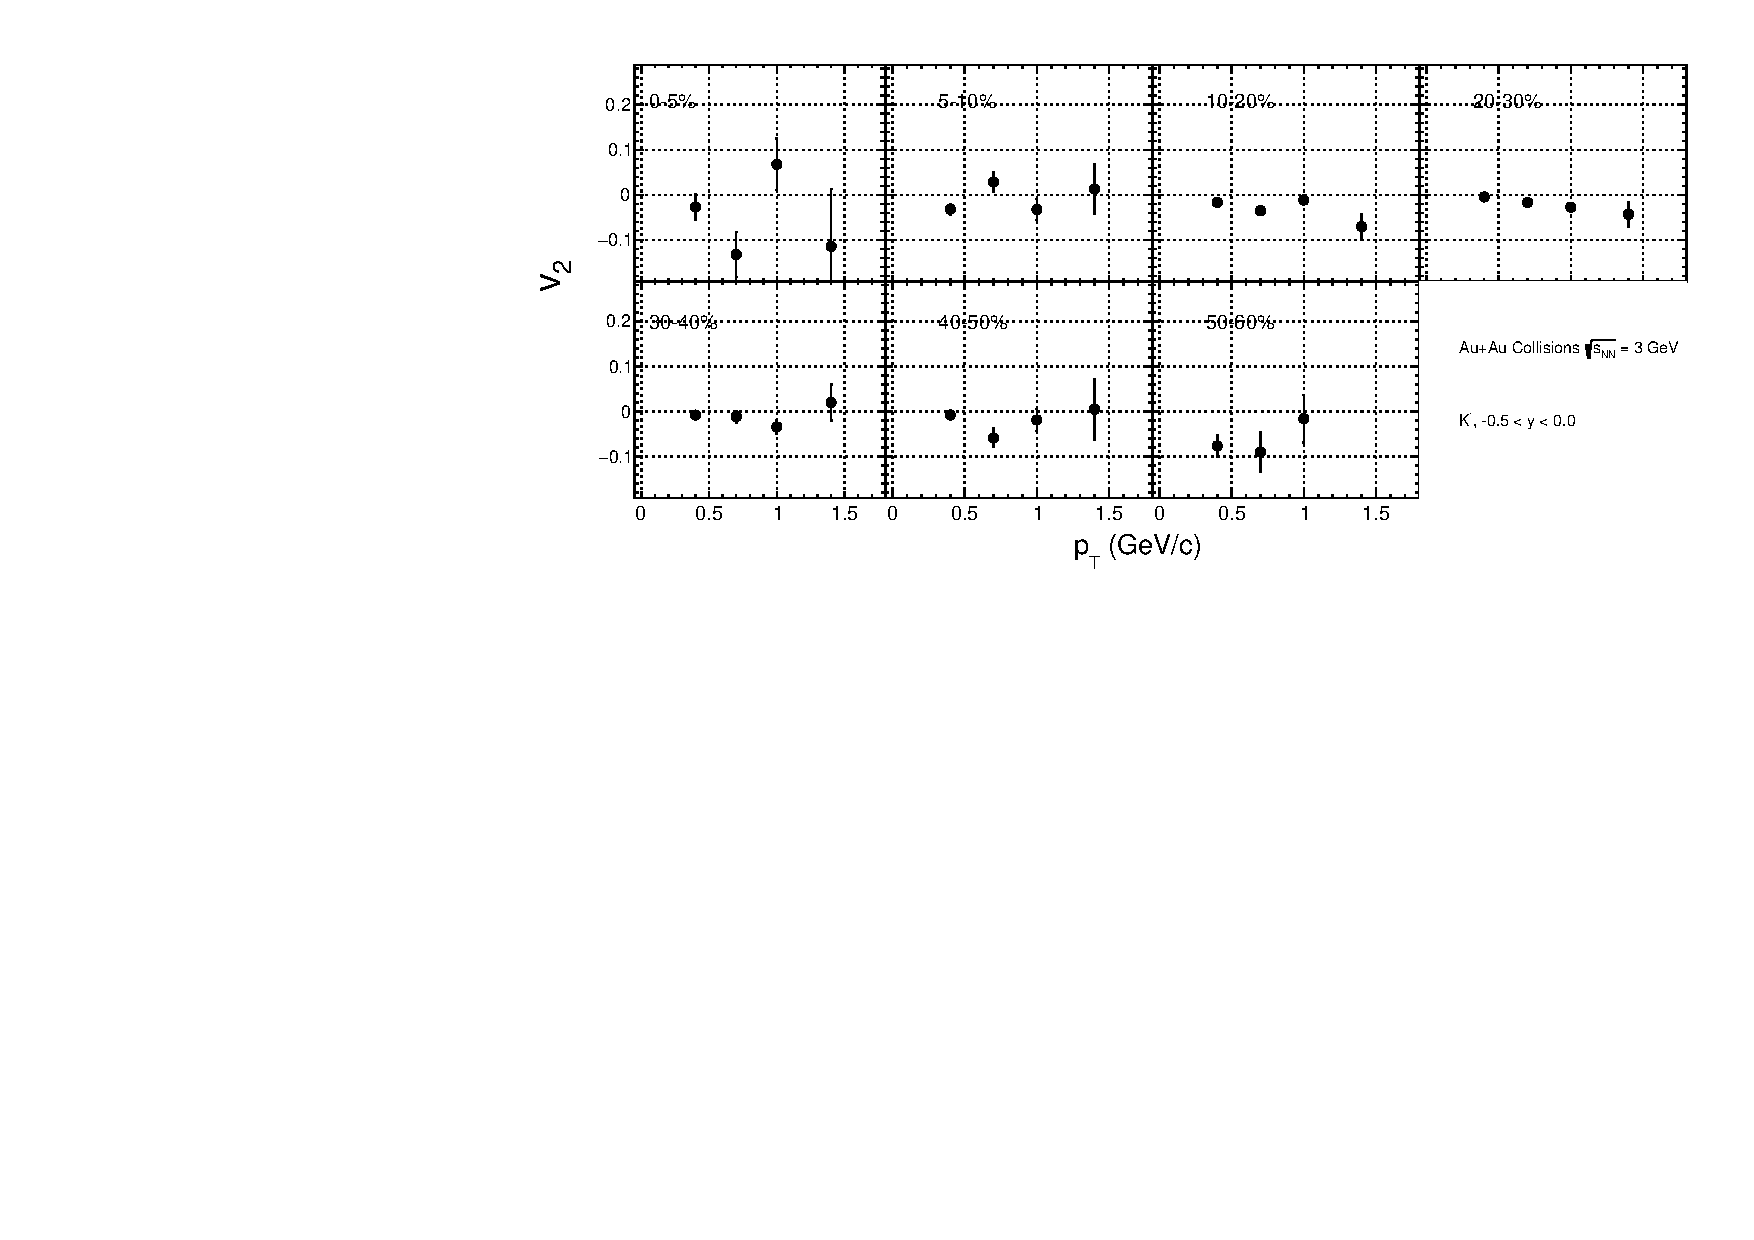
\includegraphics[scale=0.5]{chapter3/fig/v2ptpikp/v2pt_cent_kaonm.pdf}
\caption{$v_{2}$ as a function of $p_{T}$ in different centrality bins for $K^{+}$ and $K^{-}$ in Au+Au collisions at $\sqrt{s_{NN}}$ = 3 GeV.}
\label{kaon_v2pt_cent}
\end{figure}

\begin{figure}[h]
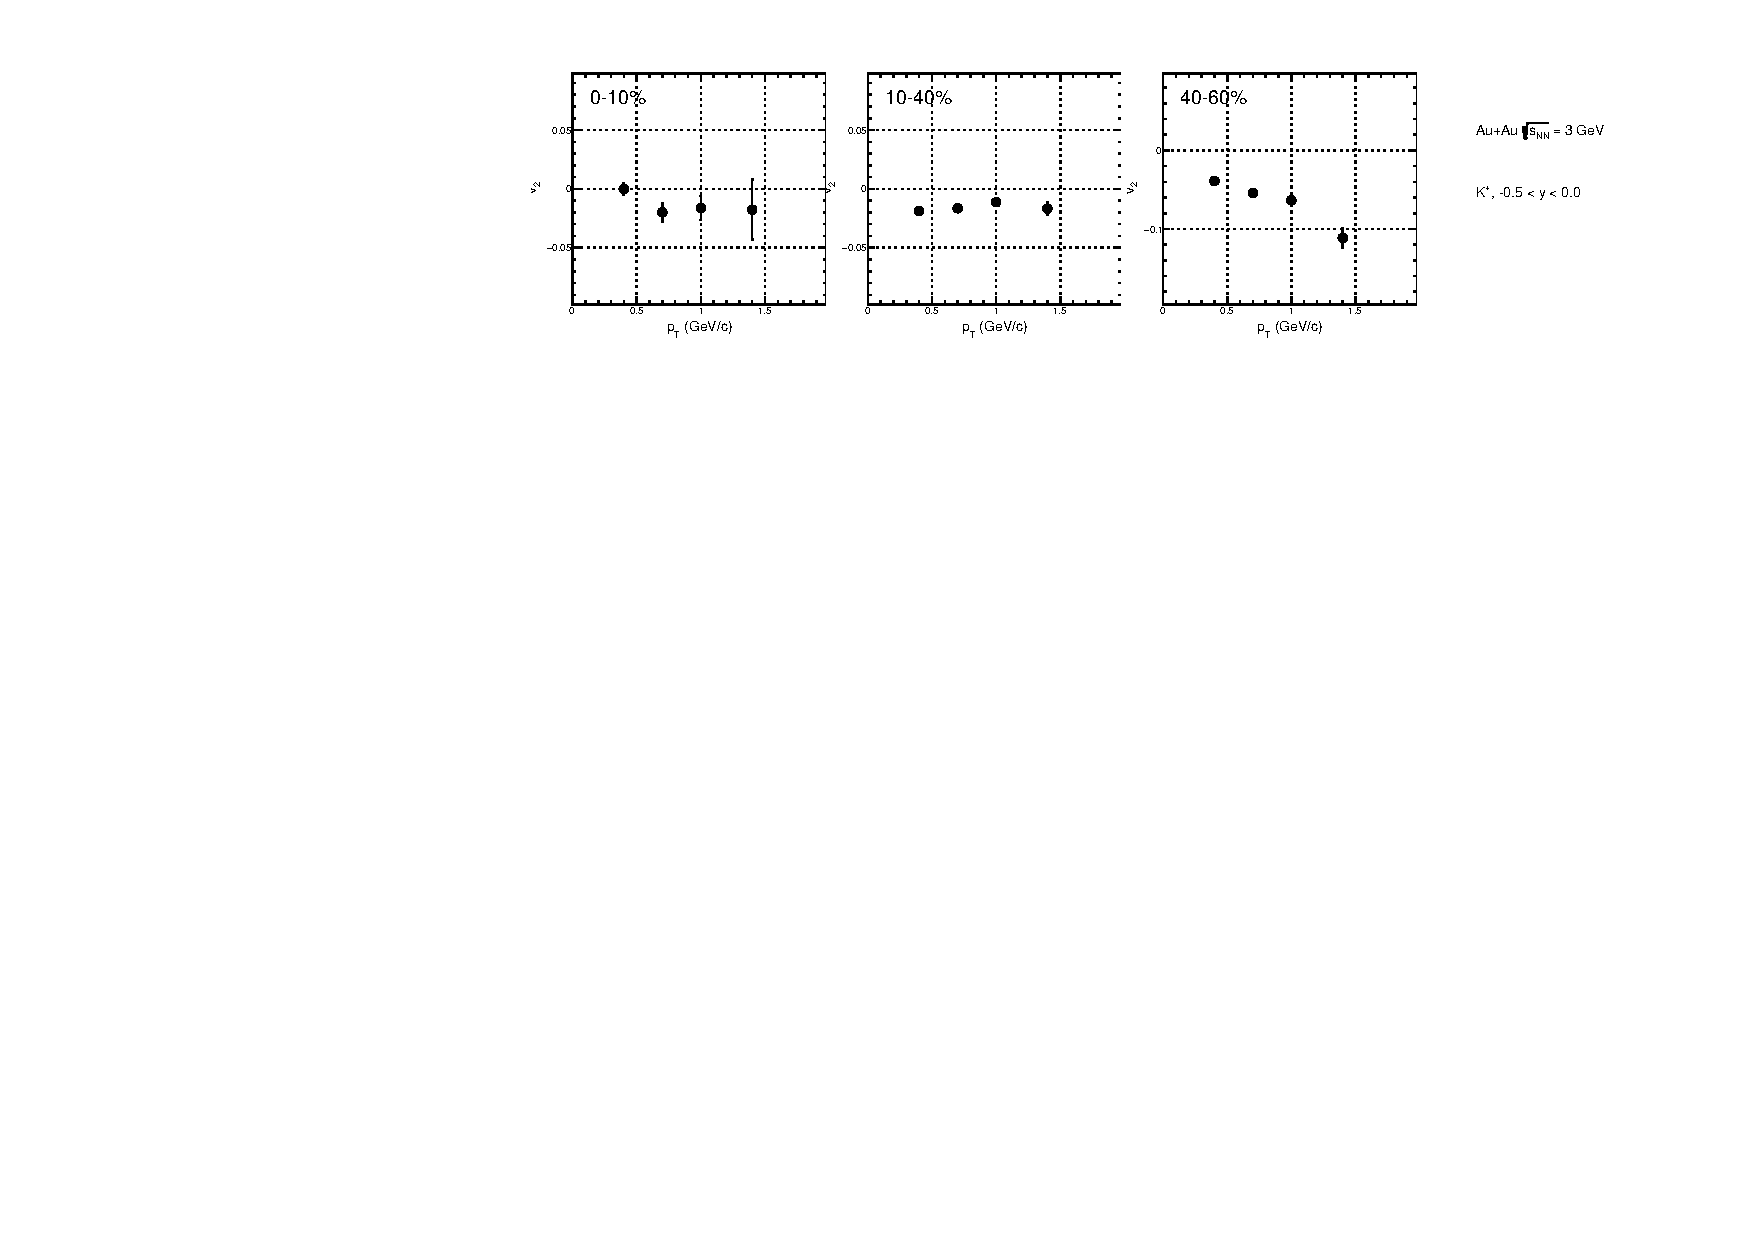
\includegraphics[scale=0.5]{chapter3/fig/v2ptpikp/kaonp_v2pt_wide_cent.pdf}
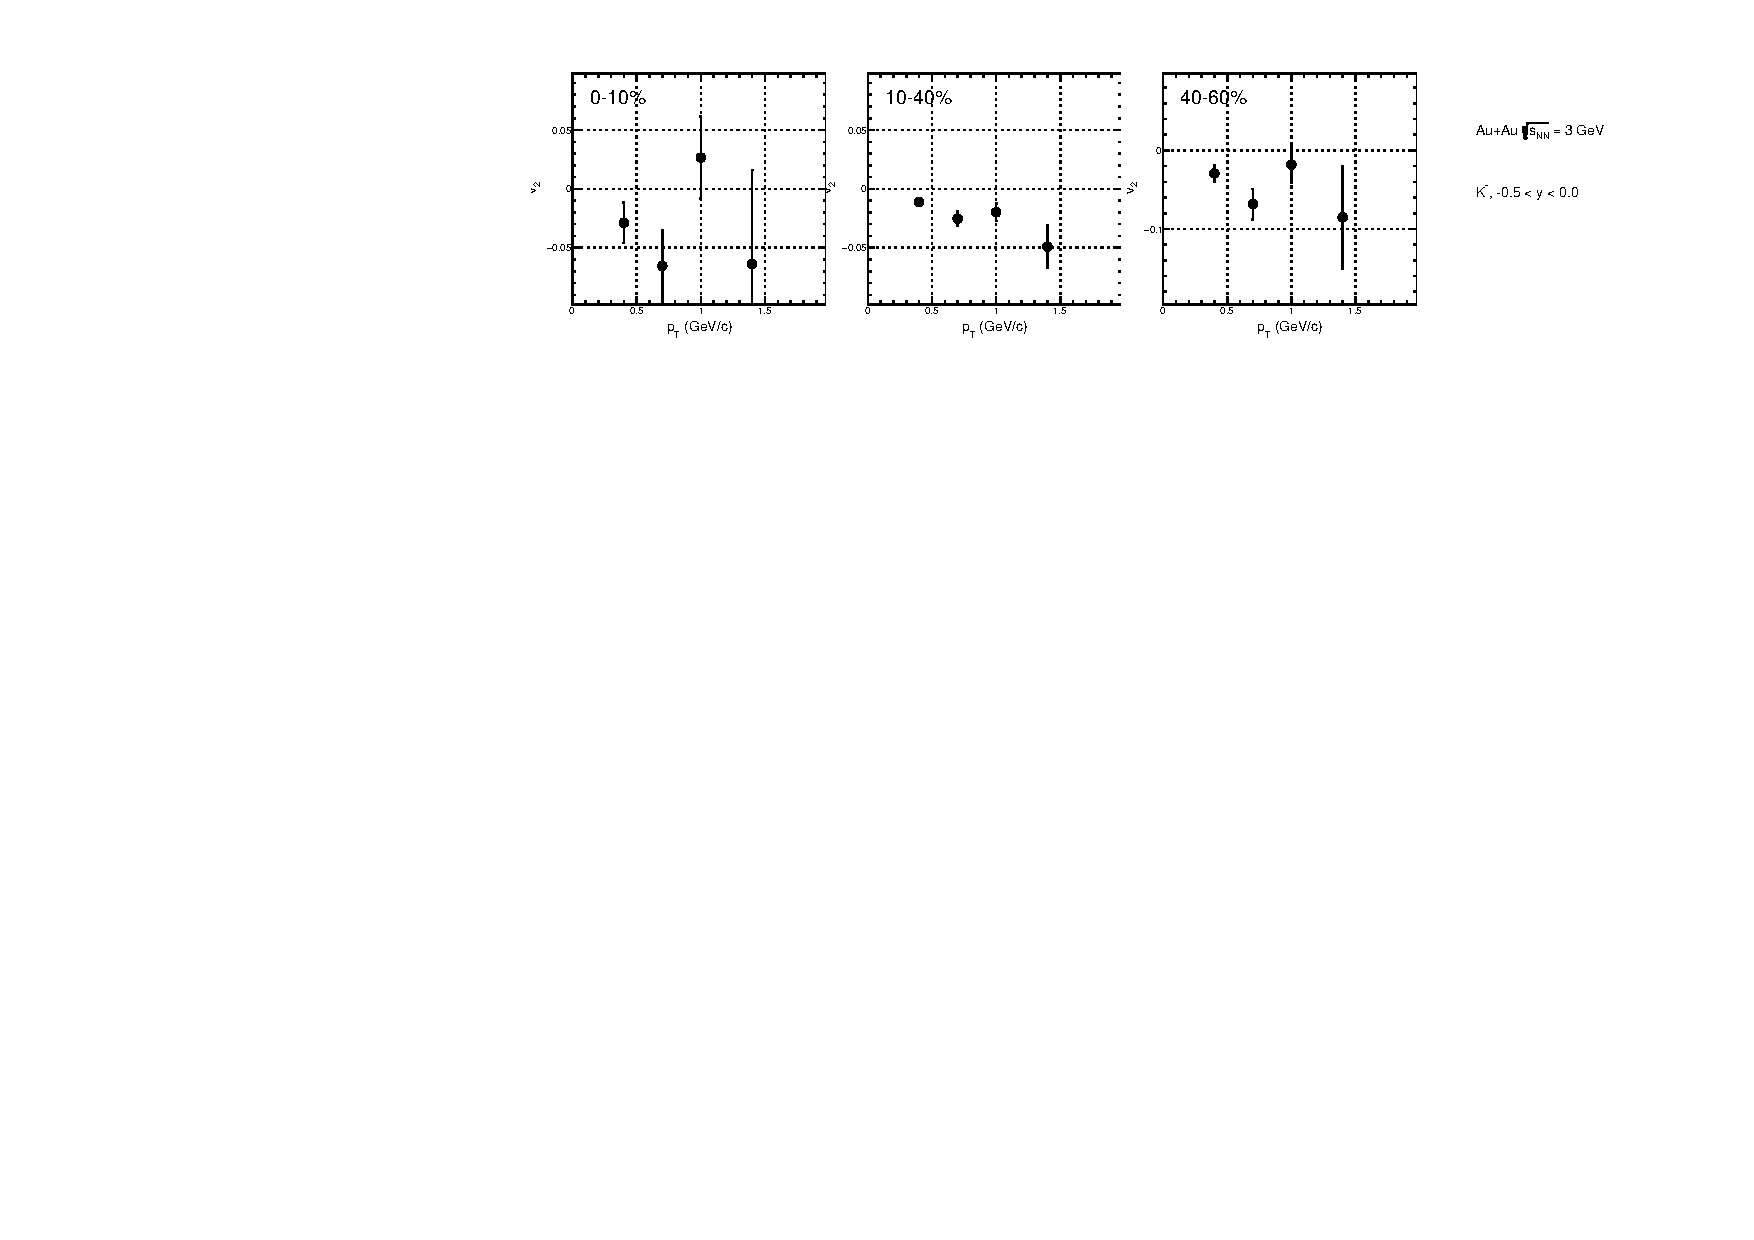
\includegraphics[scale=0.5]{chapter3/fig/v2ptpikp/kaonm_v2pt_wide_cent.pdf}
\caption{$v_{2}$ as a function of $p_{T}$ in different centrality bins for $K^{+}$ and $K^{-}$ in Au+Au collisions at $\sqrt{s_{NN}}$ = 3 GeV in 0-10\%, 10-40\%, 40-60\% centrality bins.}
\label{kaon_v2pt_widecent}
\end{figure}






\clearpage


\subsubsection{proton $v_{2}$ as a function of $p_{T}$ and rapidity}
In this chapter, we will show the results of protons' $v_{2}$ as a function of $p_{T}$ and rapidity(y).
Figure \ref{proton_v2y_cent} shows proton $v_{2}$ as a function of y for different centrality bins from 0-5\% to 50-60\%. The $p_{T}$ range is [0.4, 2.0] GeV/c. Figure \ref{proton_v2y_widecent} shows the proton’s $v_{2}$ vs. y in wider centrality bin. As we can see, proton $v_{2}$ is negative at mid-rapidity region. In 0-10\% and 10-40\% centrality bin, proton $v_{2}$ is negative at mid-rapidity region, while is positive at forward rapidity region.



\begin{figure}[h]
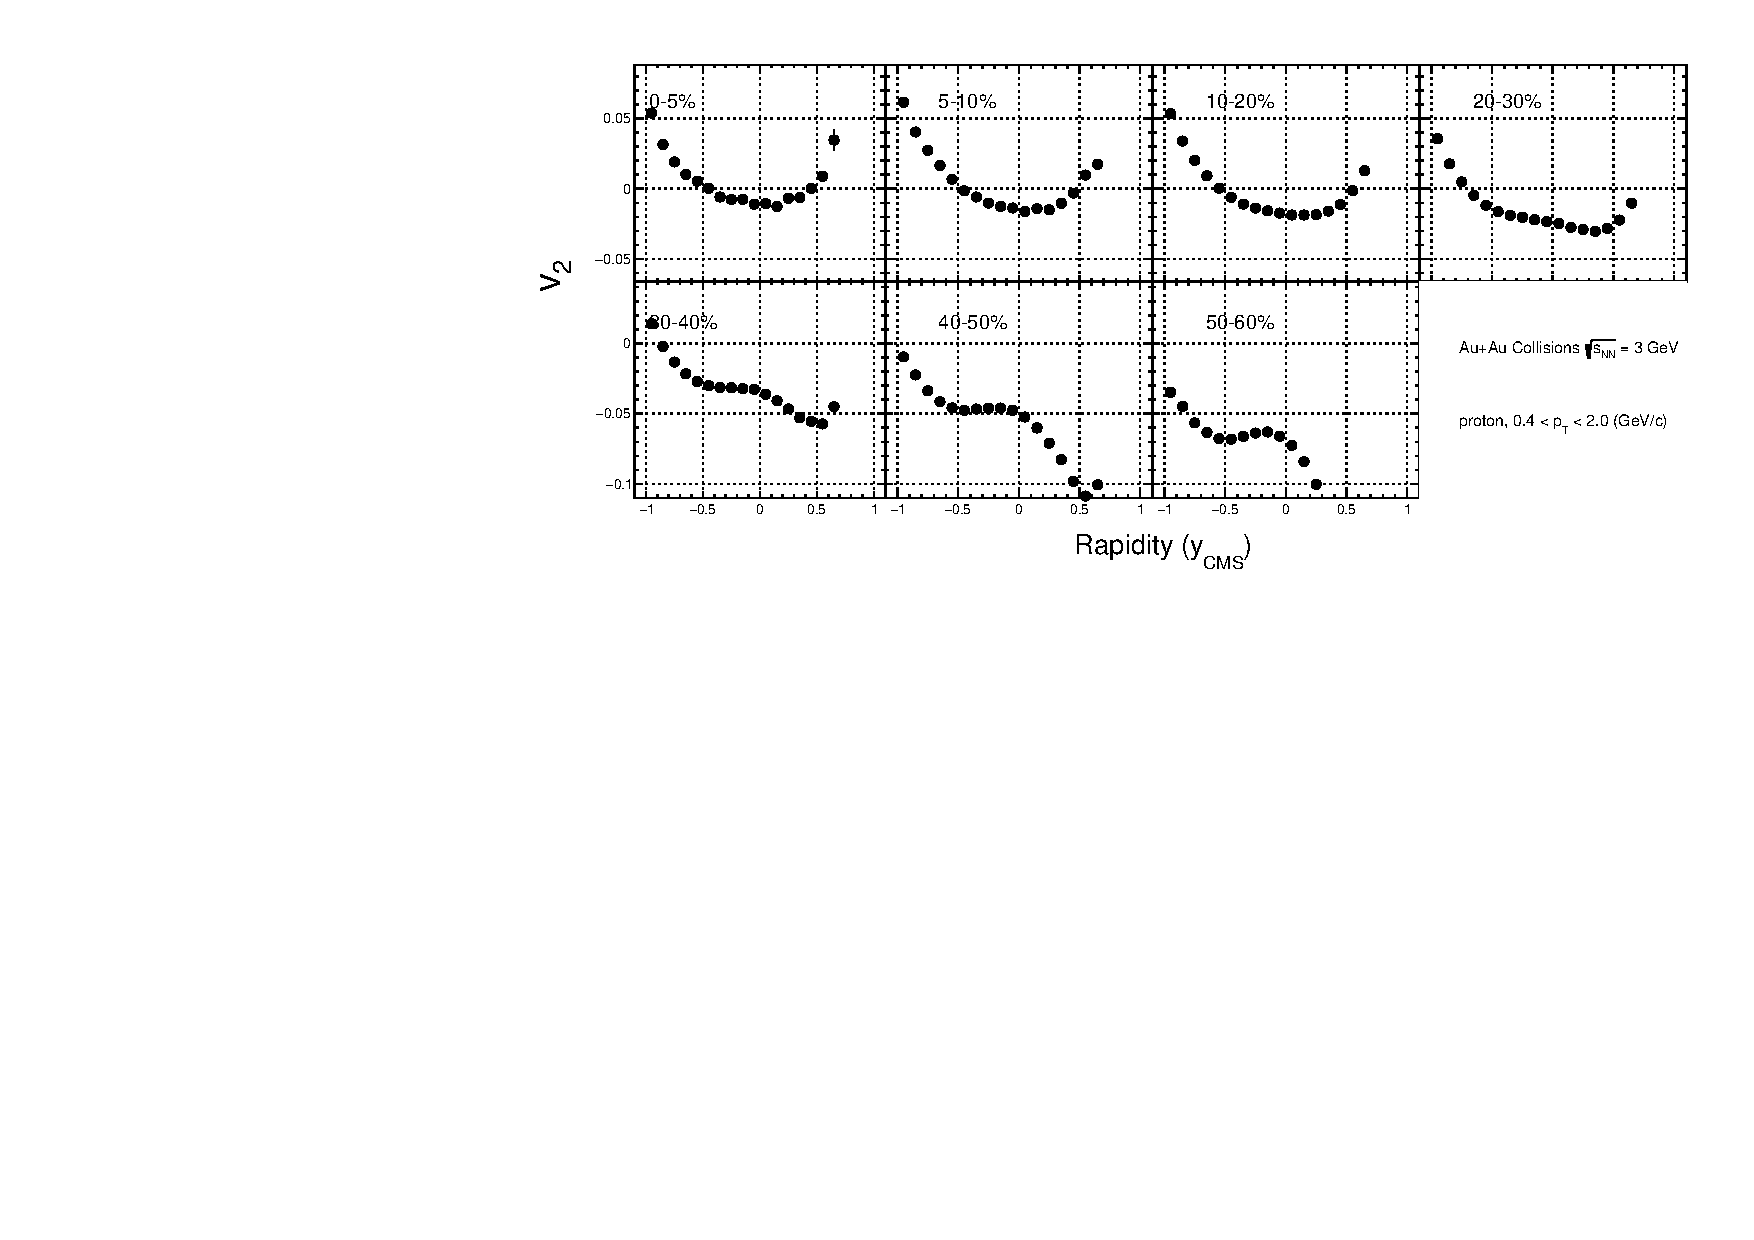
\includegraphics[scale=0.6]{chapter3/fig/v2ypikp/v2y_cent_proton.pdf}
\caption{proton $v_{2}$ as a function of rapidity(y) in different centrality bins in Au+Au collisions at $\sqrt{s_{NN}}$ = 3 GeV.}
\label{proton_v2y_cent}
\end{figure}

\begin{figure}[h]
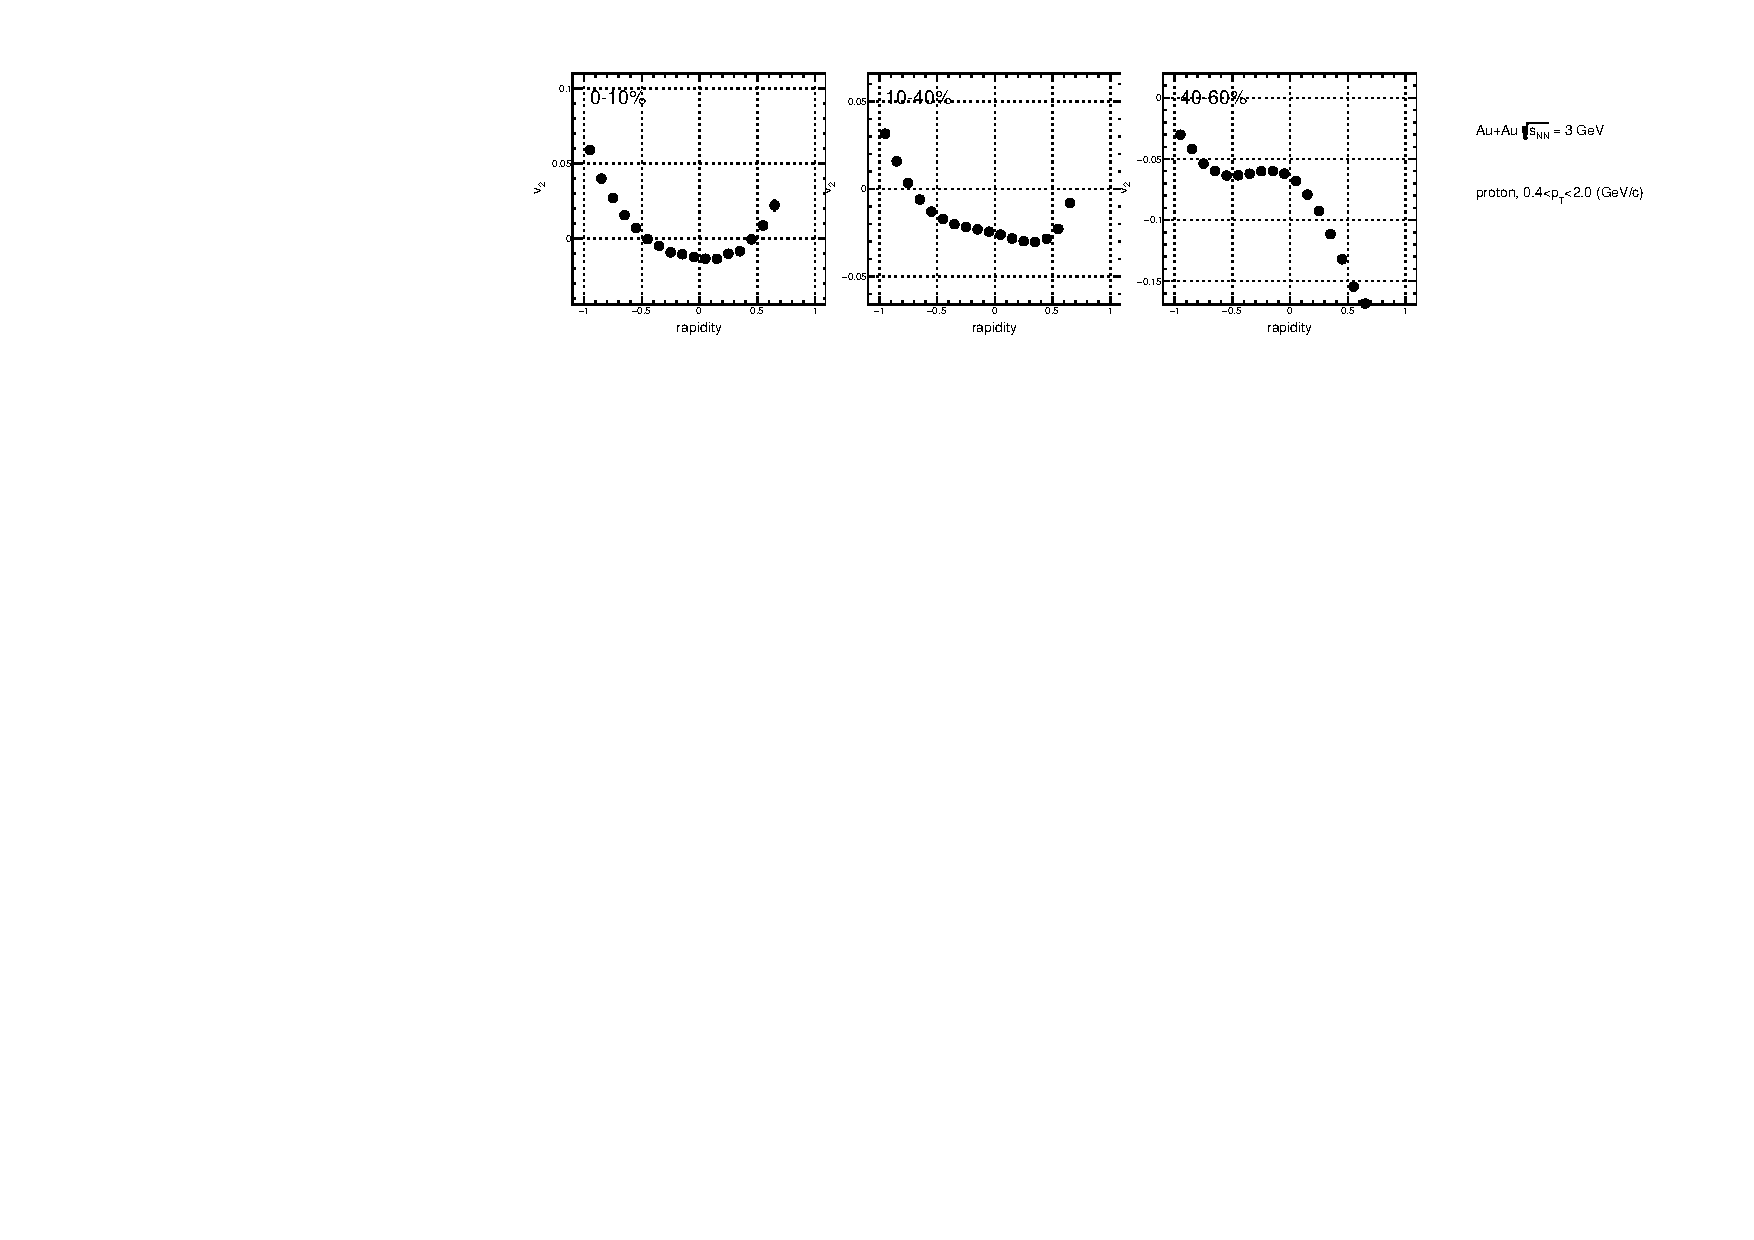
\includegraphics[scale=0.6]{chapter3/fig/v2ypikp/protonp_v2y_wide_cent.pdf}
\caption{proton $v_{2}$ as a function of rapidity(y) in different centrality bins for in Au+Au collisions at $\sqrt{s_{NN}}$ = 3 GeV in 0-10\%, 10-40\%, 40-60\% centrality bins.}
\label{proton_v2y_widecent}
\end{figure}

We also study the $p_{T}$ dependence for proton's $v_{2}$ in the figure \ref{proton_v2pt_cent}, as we can see, proton's $v_{2}$ is decreasing with $p_{T}$ increasing. Figure \ref{proton_v2pt_widecent} shows these results in wider centrality bins 0-10\%, 10-40\%, 40-60\%. The proton $v_{2}$ decreases with $p_{T}$ increases, then proton $v_{2}$ increases at higher $p_{T}$ region.


\begin{figure}[h]
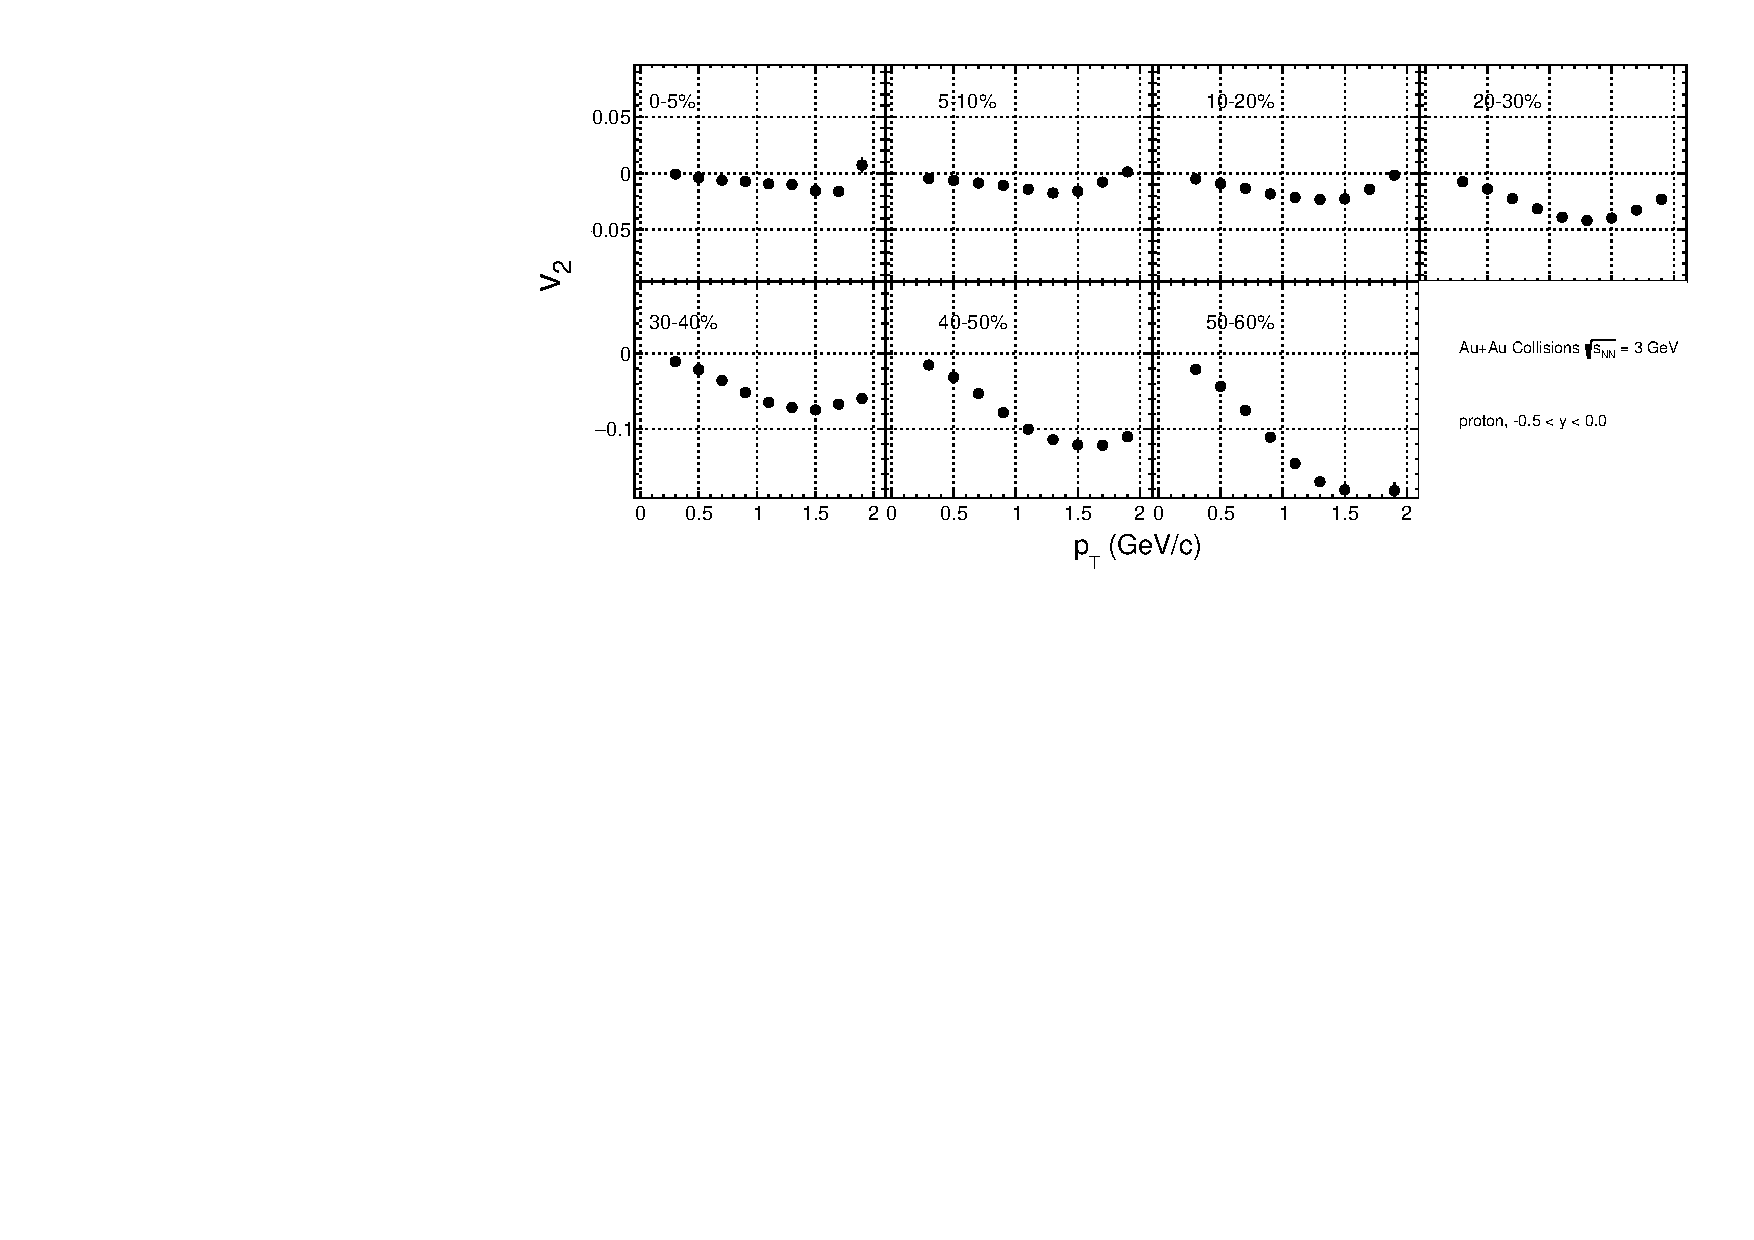
\includegraphics[scale=0.6]{chapter3/fig/v2ptpikp/v2pt_cent_proton.pdf}
\caption{proton $v_{2}$ as a function of $p_{T}$ in different centrality bins in Au+Au collisions at $\sqrt{s_{NN}}$ = 3 GeV.}
\label{proton_v2pt_cent}
\end{figure}

\begin{figure}[h]
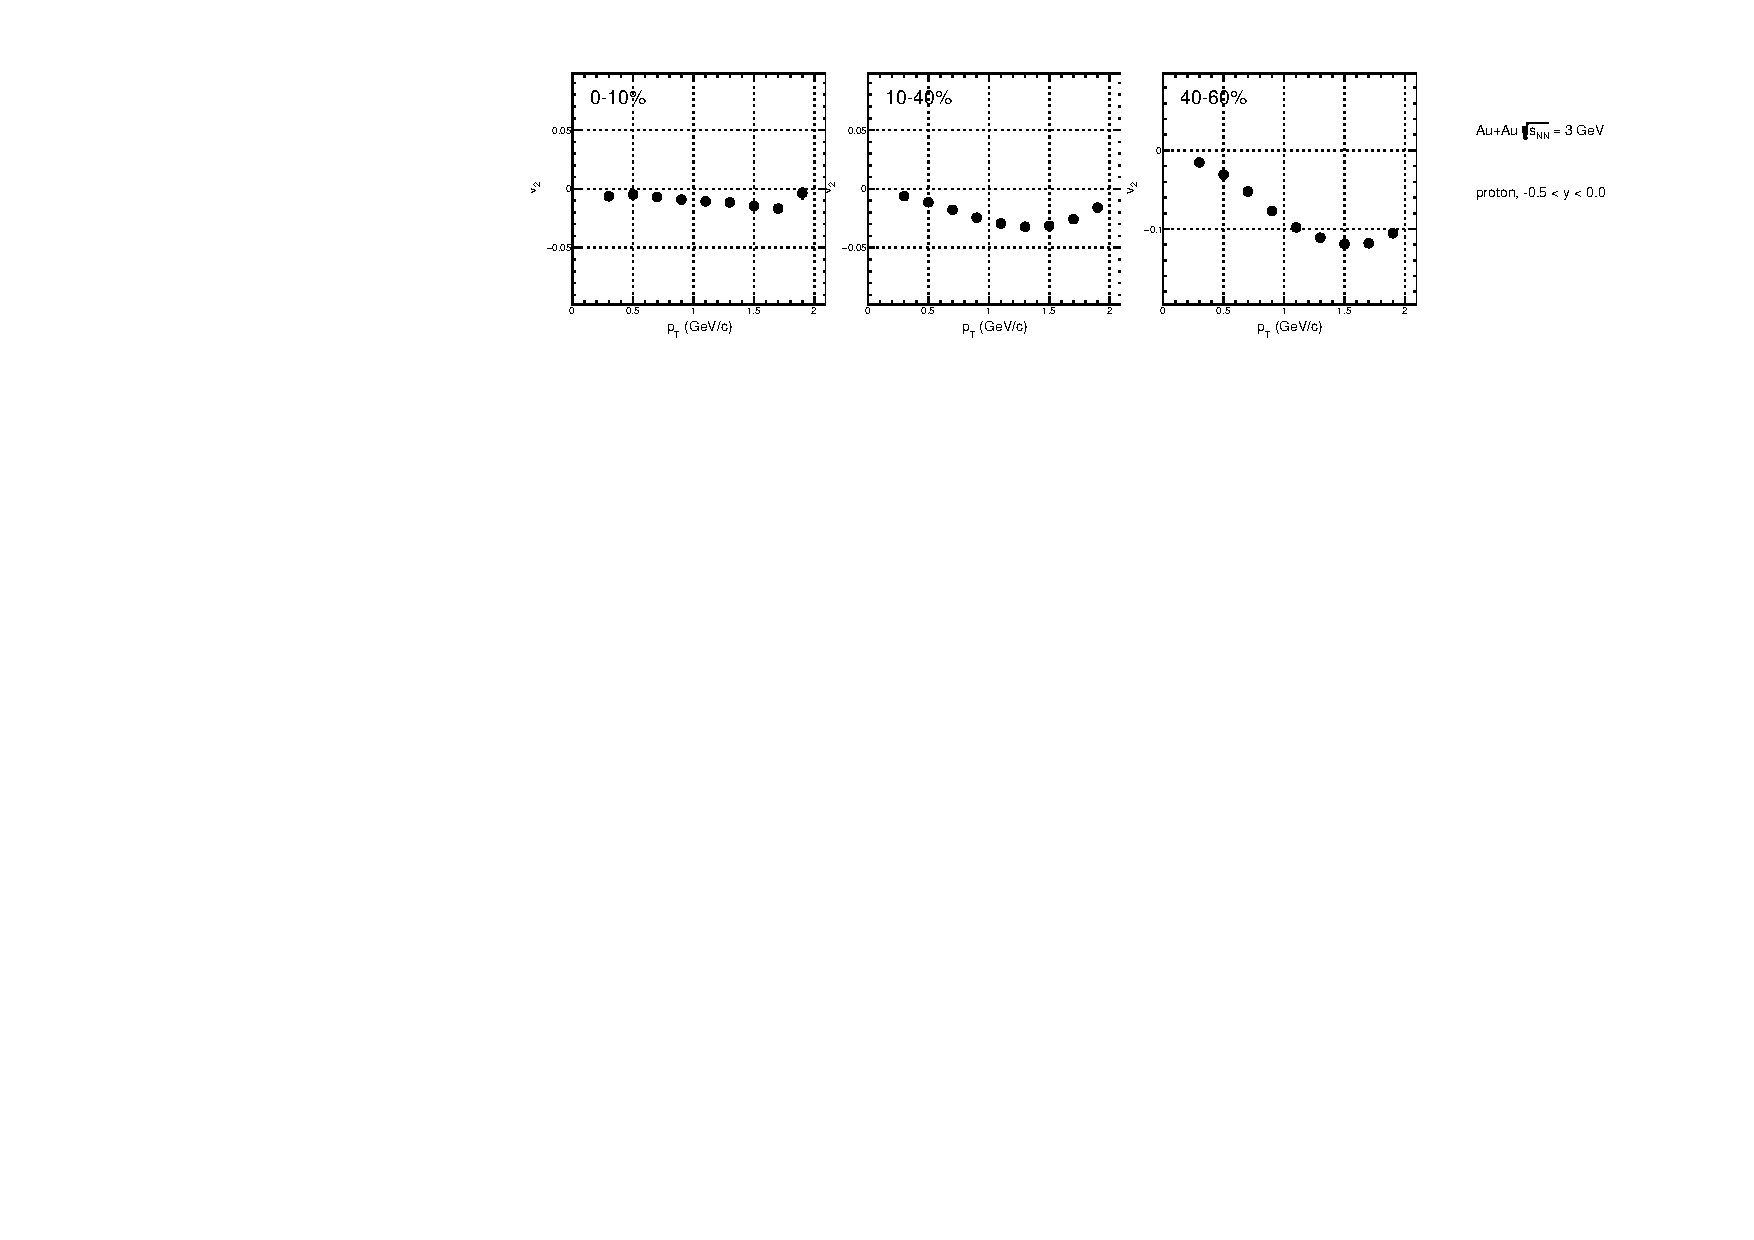
\includegraphics[scale=0.6]{chapter3/fig/v2ptpikp/protonp_v2pt_wide_cent.pdf}
\caption{proton $v_{2}$ as a function of $p_{T}$ in different centrality bins in Au+Au collisions at $\sqrt{s_{NN}}$ = 3 GeV in 0-10\%, 10-40\%, 40-60\% centrality bins.}
\label{proton_v2pt_widecent}
\end{figure}

\clearpage
\newpage

\subsection{$v_{2}$ from second order event plane}
As discussed in the second chapter, the $v_{2}$ is calculated from first order event plane angle $\Psi_{1}$, this is because the higher first order event plane resolution (up to 70\%) than second order resolution, which will induce the higher lower error bar for $v_{2}$, and numerically it is equivalent to that we use second order event plane angle $\Psi_{2}$ to calculate $v_{2}$. The different order event plane resolution comparison can be found in the figure \ref{res2_tpc_epd}.
Here in the figure \ref{psi2_dis_tpc_epd}, we show the reconstructed second order event plane angle distribution in different centrality in different sub-event group of TPC and EPD. The black line is raw $\Psi_{2}$ distribution, the blue line is $\Psi_{2}$ distribution with re-centering calibration and red line is $\Psi_{2}$ distribution with re-centering and shift calibration,  as we can see, after re-centeringing and shift calibration (the red line) we have flat second order event plane angle $\Psi_{2}$ distribution, and it can be used for $v_{2}$ calculation. 

\begin{figure}[h]
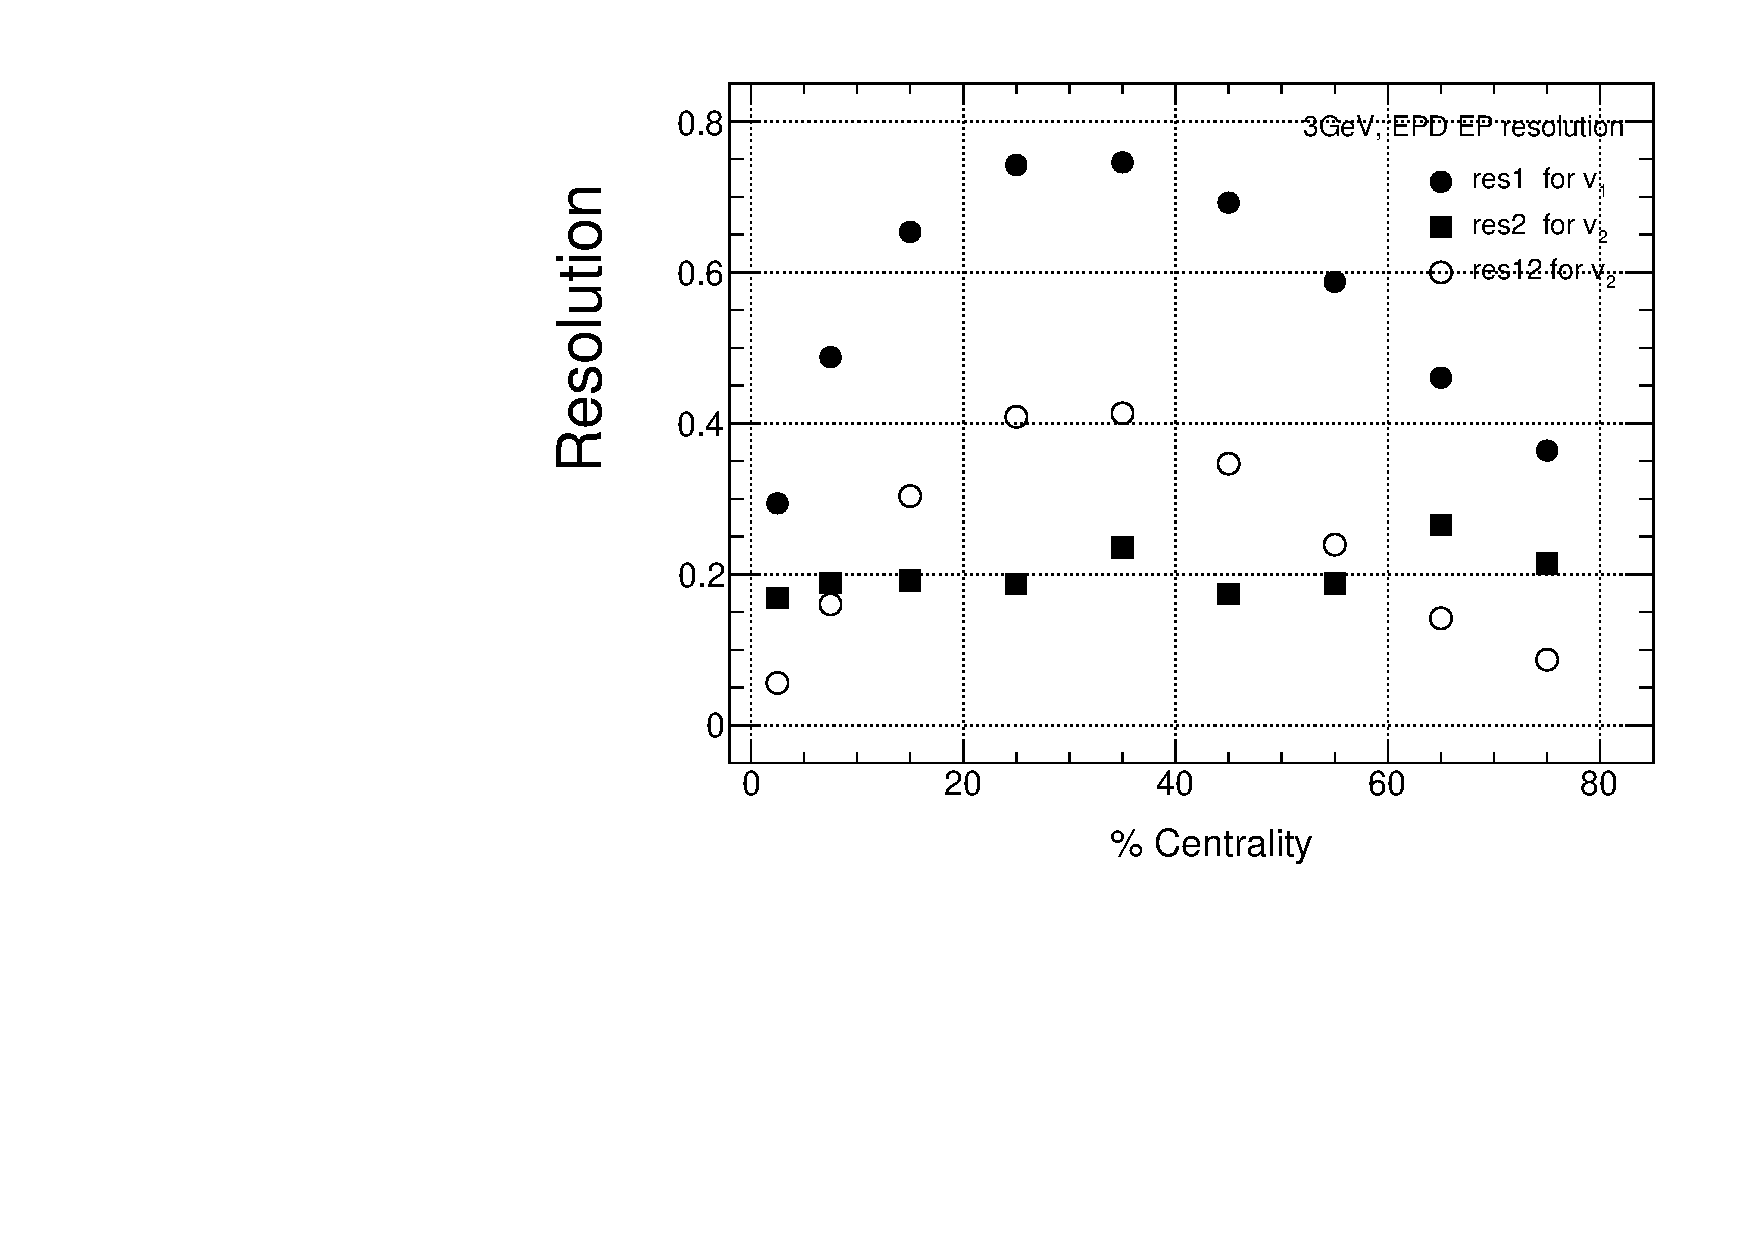
\includegraphics[scale=0.6]{chapter3/fig/second/res_3gev_com.pdf}
\caption{\label{res2_tpc_epd} EPD event plane resolution as a function of collision centrality, the black solid circle is first order event plane resolution, black open circle is the converted second order event plane resolution for $v_{2}$ calculation, the black solid square is second order event plane resolution.}
\end{figure}

\begin{figure}[h]
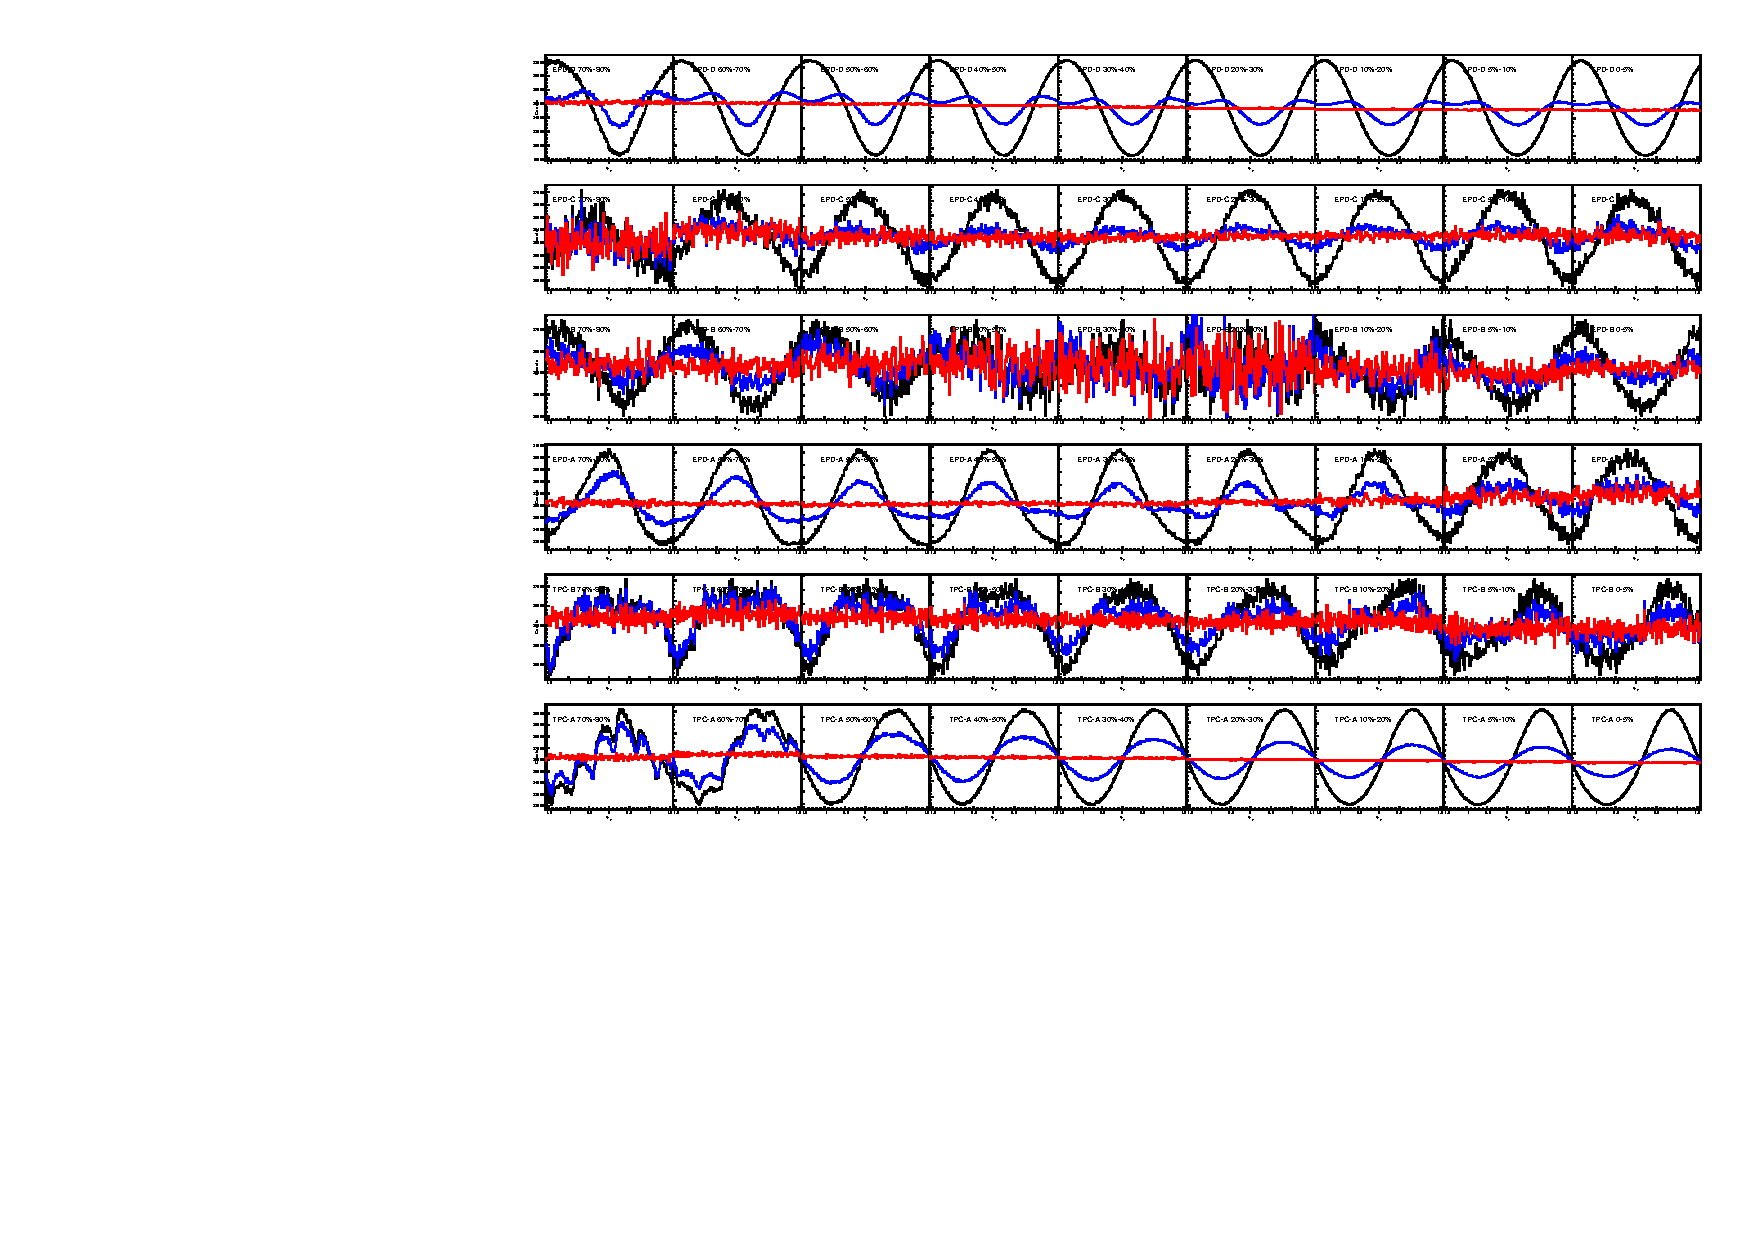
\includegraphics[scale=0.6]{chapter3/fig/second/psi2.pdf}
\caption{\label{psi2_dis_tpc_epd} TPC and EPD sub-event plane angle ($\Psi_{2}$) distribution in different centralities, the black line is raw $\Psi_{2}$ distribution, the blue line is $\Psi_{2}$ distribution with re-centering calibration, the red line is $\Psi_{2}$ distribution with re-centering and shift calibration.}
\end{figure}

We calculate the proton $v_{2}$ as a function of $p_{T}$ using second order event plane angle $\Psi_{2}$ and make comparison to the results from using first order event plane angle. It can be found in the figure \ref{v2pt_sec_com}. We found their results are consistent in the low $p_{T}$ and middle $p_{T}$ region. There is little difference in the high $p_{T}$ region, we think this could be some effect from proton's purity, and the error is also too large. So far, our conclusion is that the results of $v_{2}$ using first order and second event plane angle are consistent.

\begin{figure}[h]
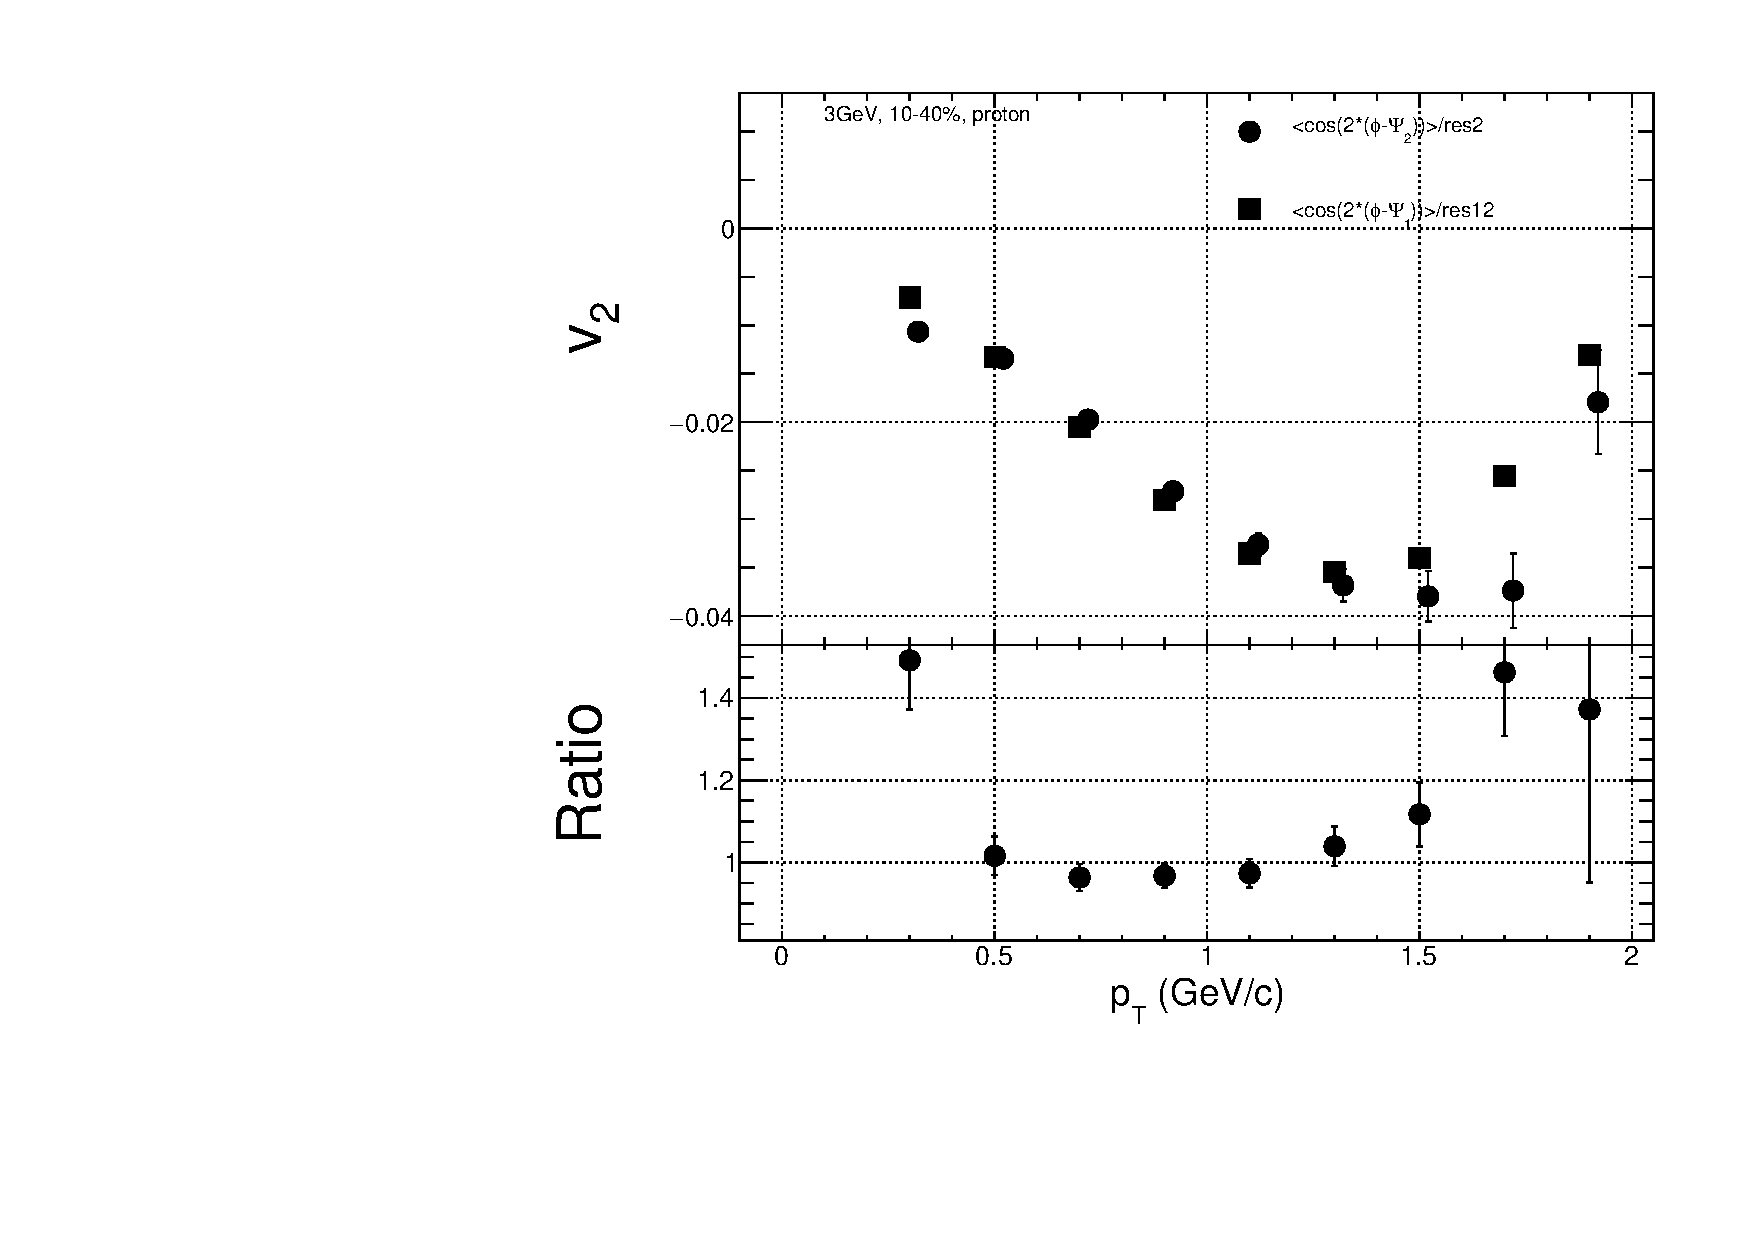
\includegraphics[scale=0.6]{chapter3/fig/second/v2pt_com.pdf}
\caption{\label{v2pt_sec_com} $v_{2}$ as a function of $p_{T}$ in 3GeV Au+Au collisions, 10-40\% centrality from first order and second event plane angle, and their ratio.}
\end{figure}

In order to confirm this, we also do the same analysis (calculate $v_{2}$ using first order and second order event plane angle) using UrQMD model. First, we show the resolution of different order event plane in the figure \ref{urqdm_res2}, we have the same conclusion with data, the second order event plane resolution is quite small than first order event plane resolution, which will induce larger error bar when calculating $v_{2}$. In the figure \ref{v2pt_urqmd_com}, we calculate the $v_{2}$ from first order and second event plane angle and make comparison. 
We found they are consistent within the error bar.

\begin{figure}[h]
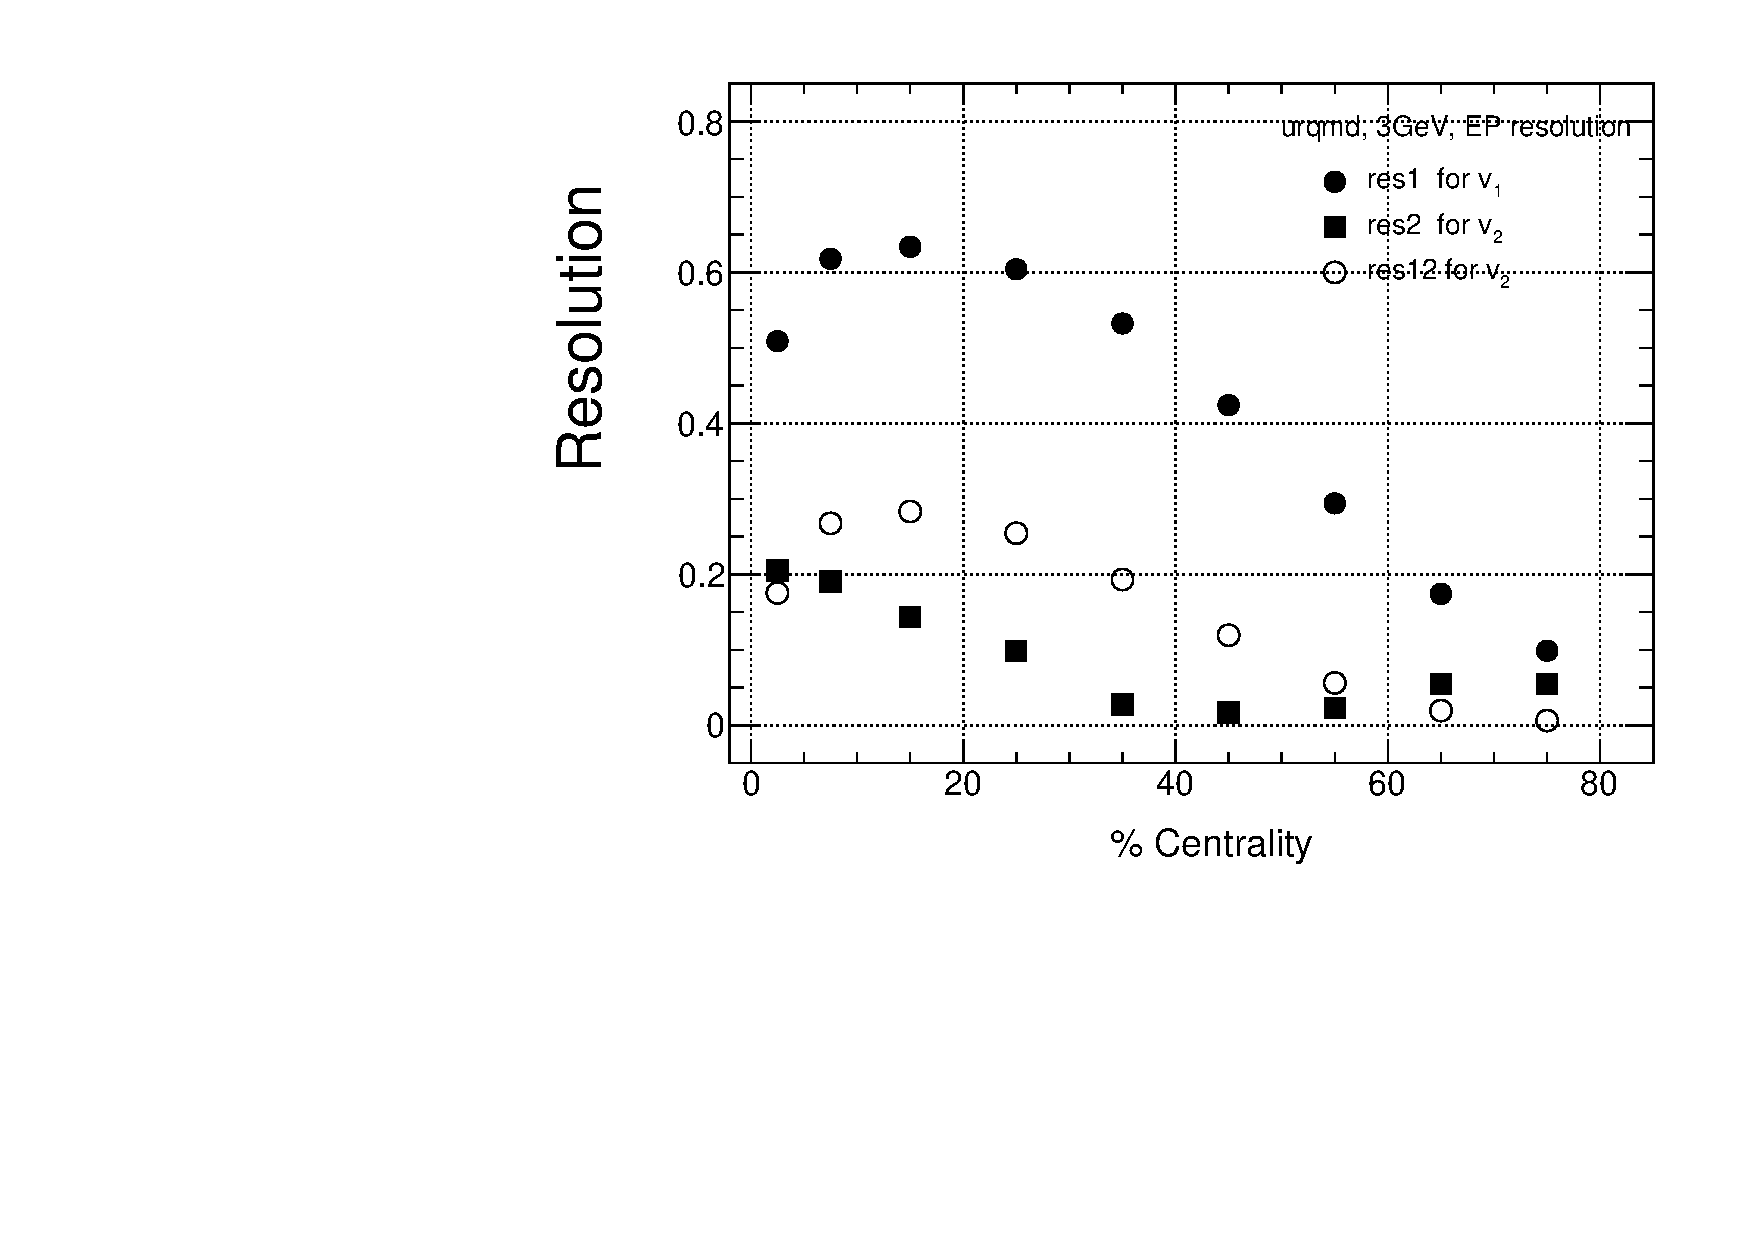
\includegraphics[scale=0.6]{chapter3/fig/second/res_urqmd.pdf}
\caption{\label{urqmd_res2} The event plane resolution as a function collision centrality at 3GeV in UrQMD model for first order second order and converted second order.}
\end{figure}

\begin{figure}[h]
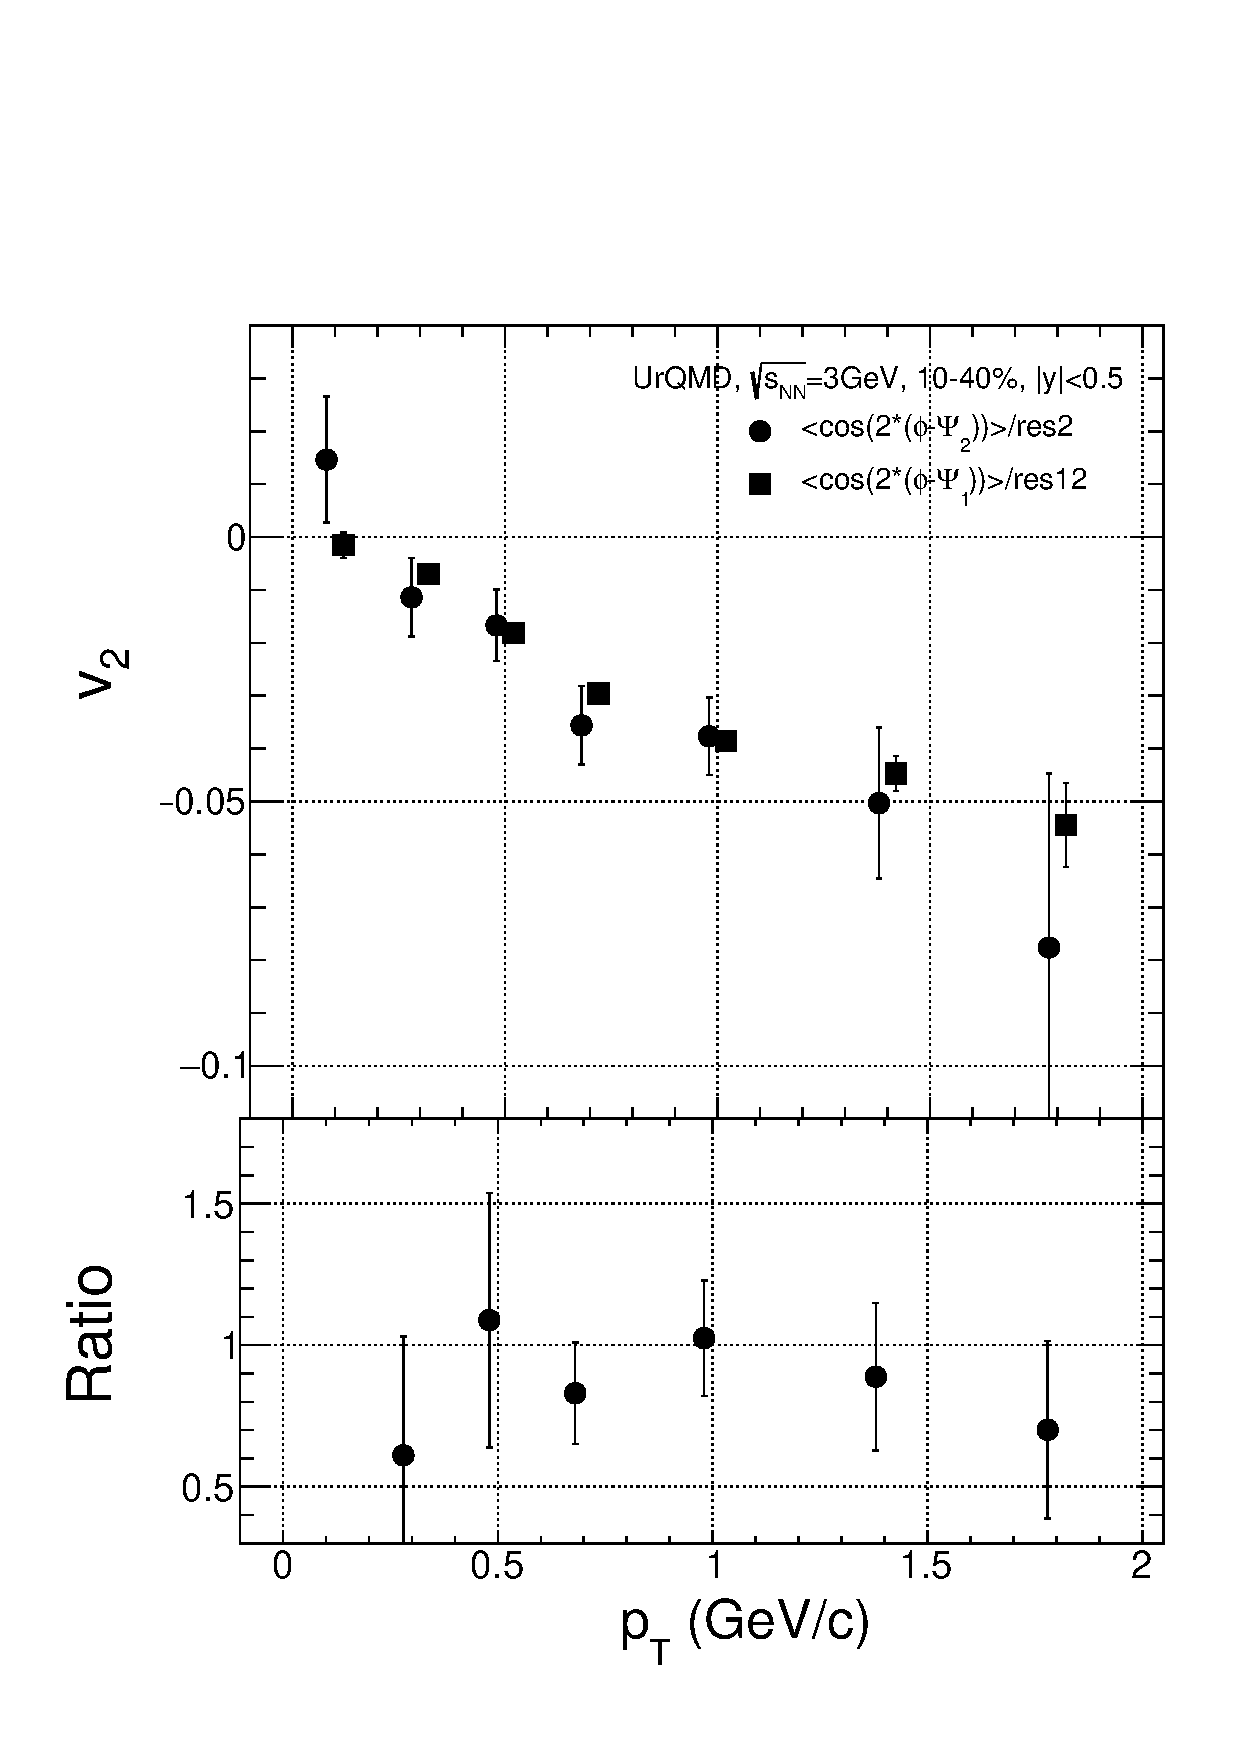
\includegraphics[scale=0.6]{chapter3/fig/second/v2pt_urqdm.pdf}
\caption{\label{v2pt_urqmd_com} $v_{2}$ as a function of $p_{T}$ at 3 GeV 10-40\% in UrQMD model from first order and second event plane angle, and their ratio.}
\end{figure}


\clearpage
\subsection{Systematic Uncertainties}

Point-by-point systematic errors on variables used for tracks cuts and particle identification and resolution. For all systematic checks, the various cuts are changed one at a time. Table \ref{sys_cut_pionkaon} shows the systematic cuts and minimum and maximum values used in the analysis for pions and kaons. Similarly, table \ref{sys_cut_proton} shows the systematic cuts used in the analysis for proton. 
For each cut variable, we choose the maximum deviation from default value, then the total systematic uncertainty can be estimated using in the equation \ref{sys_equation} from different source (dca, nHitsFit, n$\sigma_{particle}$, resolution, efficiency). The systematic uncertainty contribution from event plane or resolution should be constants for all particles. in 10-40\% centrality bin, the systematic uncertainty contribution from event plane is 1.4\% for $v_{1}$ and 3\% for $v_{2}$. \ref{tab:syserr_dv1dy} lists the relative systematic uncertainty contribution from different cut and the total systematic uncertainty for $dv_{1}/dy$.

\begin{equation}
	sys_{total}=\sqrt{(y_{dca}-y_{def})^{2} + (y_{nHit}-y_{def})^{2} + (y_{n\sigma}-y_{def})^{2} + (y_{EP}-y_{def})^{2} + (y_{eff}-y_{def})^{2}}
\label{sys_equation}
\end{equation}

\begin{table}[ht]
\caption{Systematic cuts for pions and kaons}
\label{sys_cut_pionkaon}
\begin{tabular}{cccc}
\hline
Cuts & Default & var1 & var2\\ 
\hline
dca ($<$) & 3 & 1 & 2\\ 
%\hline
nHitFit ($>$) & 15 & 10 & 20\\ 
%\hline
$|$ n$\sigma_{particle}$ $|$ $<$ & 3 & 2 & 2.5 \\ 
%\hline
resolution reference EP & EPD-C & EPD-CD & EPD D\\ 
\hline
\end{tabular} 
\end{table}


\begin{table}[ht]
\caption{Systematic cuts for proton}
\label{sys_cut_proton}
\begin{tabular}{cccc}
\hline
Cuts & Default & var1 & var2\\ 
\hline
dca ($<$) & 3 & 1 & 2\\ 
%\hline
nHitFit ($>$) & 15 & 10 & 20\\ 
%\hline
$|$ n$\sigma_{particle}$ $|$ $<$ & 2 & 3 & 2.5 \\ 
%\hline
resolution reference EP & EPD-C & EPD-CD & EPD D\\ 
\hline
\end{tabular} 
\end{table}

\begin{table}[]
    \centering
    \begin{tabular}{|c|c|c|c|c|c|c|}
    \hline
        particles & DCA & nHitsFit & $n\sigma$ & resolution & efficiency & Total \\ \hline
        $\pi^{+}$ & 3.4\% & 0.3\% & 4.3\% & 1.4\% & 0.08\% & 5.6\% \\ 
        $\pi^{-}$ & 3.5\% &0.14\% & 8.1\% & 1.4\% & 0.08\% & 8.9\% \\ 
        $K^{+}$   & 1.6\% & 0.7\% & 7.5\% & 1.4\% &  0.6\% & 7.9\% \\ 
        $K^{-}$   & 1.2\% & 4.4\% &14.5\% & 1.4\% &  2.0\% &15.4\% \\ 
        p         & 0.8\% & 0.5\% & 1.5\% & 1.4\% & 0.07\% & 2.1\% \\ 
        \hline
    \end{tabular}
    \caption{systematic uncertainty contribution from different cut for $dv_{1}/dy$}
    \label{tab:syserr_dv1dy}
\end{table}

\begin{figure}[h]
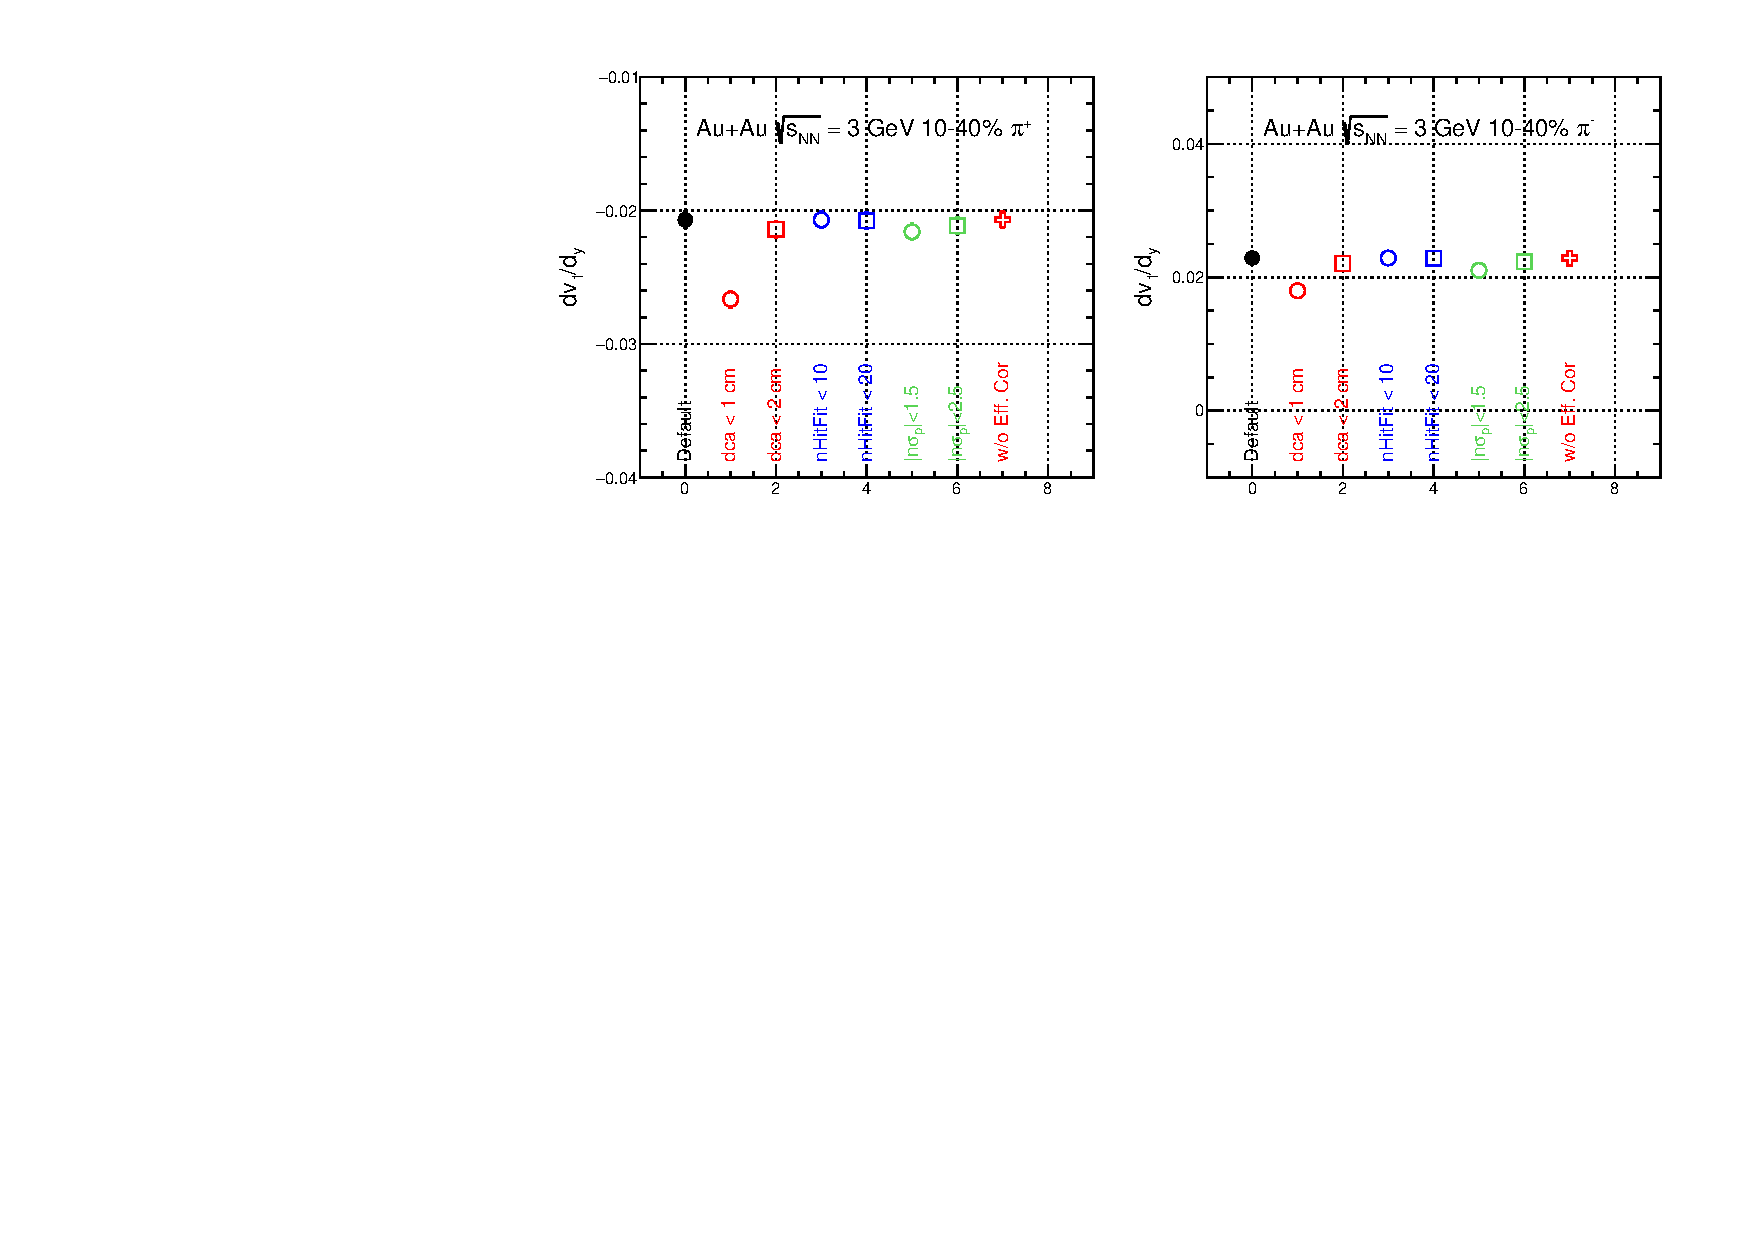
\includegraphics[scale=0.8]{FXT3gev/chapter3/fig/sys/pion/dv1y_pion_sys.pdf}
\caption{Systematic uncertainty study from different source cut for $dv_{1}/dy$ in 10-40\% for pion at $\sqrt{s_{NN}}$ = 3 GeV for $\pi^{+}$ (right) and $\pi^{-}$ (left).}
\label{fig:pion_dv1y_sys}
\end{figure}

\begin{figure}[h]
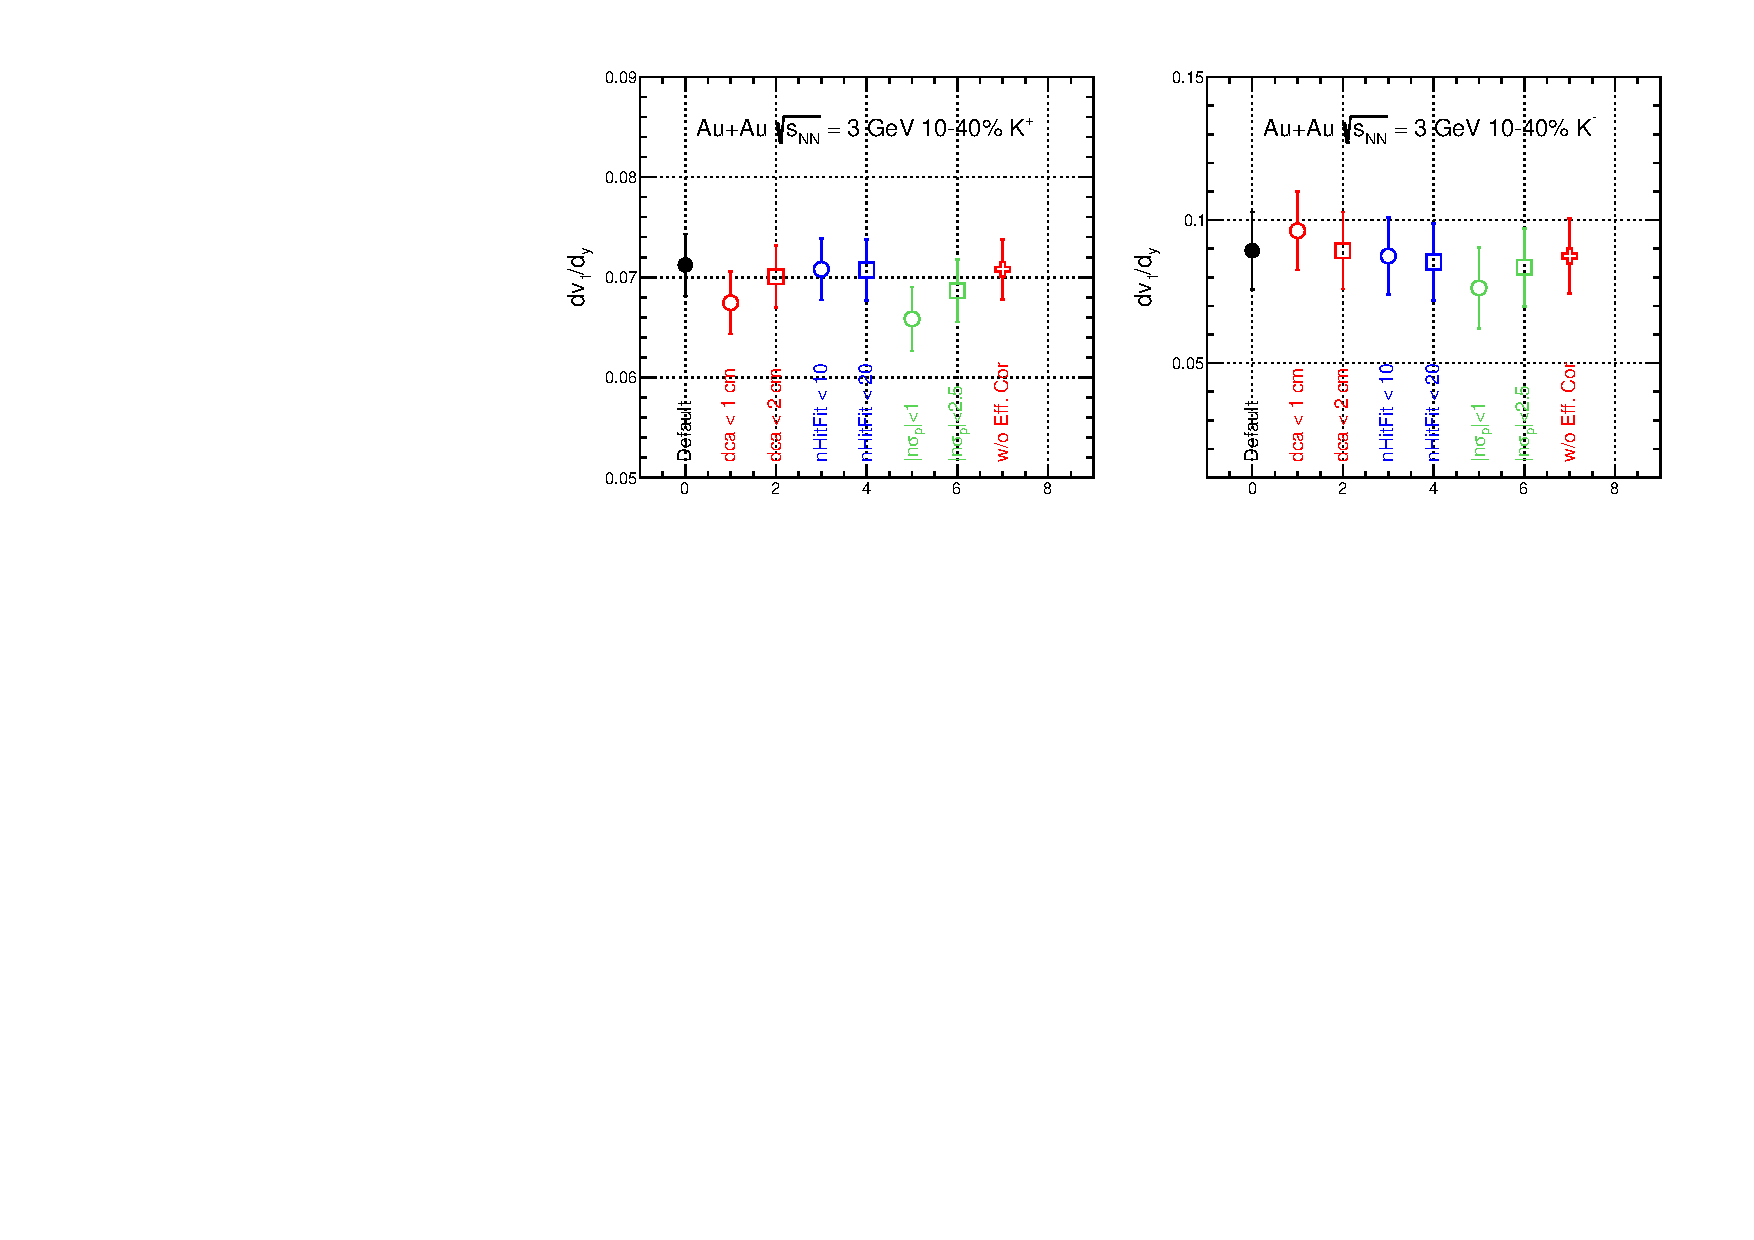
\includegraphics[scale=0.8]{FXT3gev/chapter3/fig/sys/kaon/dv1y_kaon_sys.pdf}
\caption{Systematic uncertainty study from different source cut for $dv_{1}/dy$ in 10-40\% for kaon at $\sqrt{s_{NN}}$ = 3 GeV for $K^{+}$ (right) and $K^{-}$ (left).}
\label{fig:kaon_dv1y_sys}
\end{figure}

\begin{figure}
    \centering
    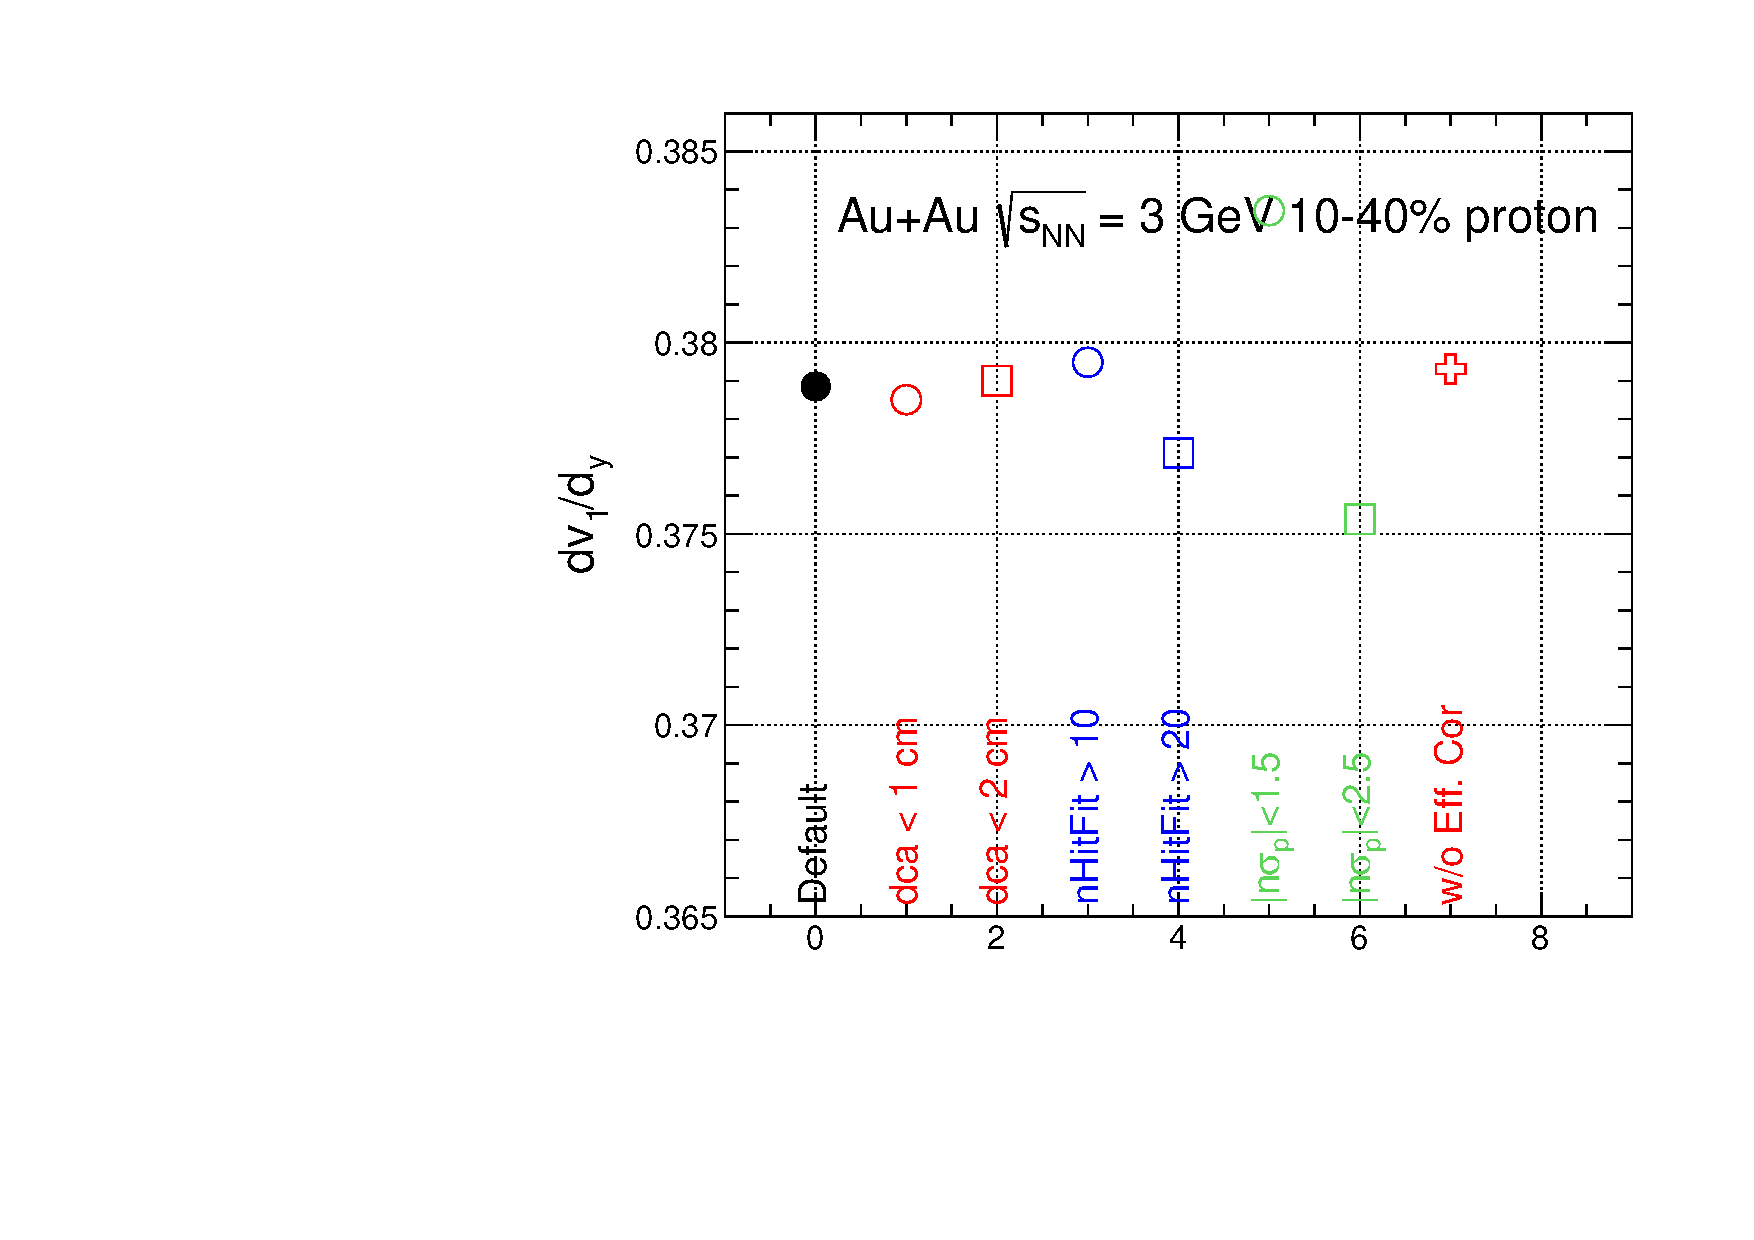
\includegraphics[scale=0.5]{FXT3gev/chapter3/fig/sys/proton/dv1y_proton_sys.pdf}
    \caption{Systematic uncertainty study from different source cut for $dv_{1}/dy$ in 10-40\% for proton at $\sqrt{s_{NN}}$ = 3 GeV}
    \label{fig:proton_dv1_sys}
\end{figure}

\begin{figure}[h]
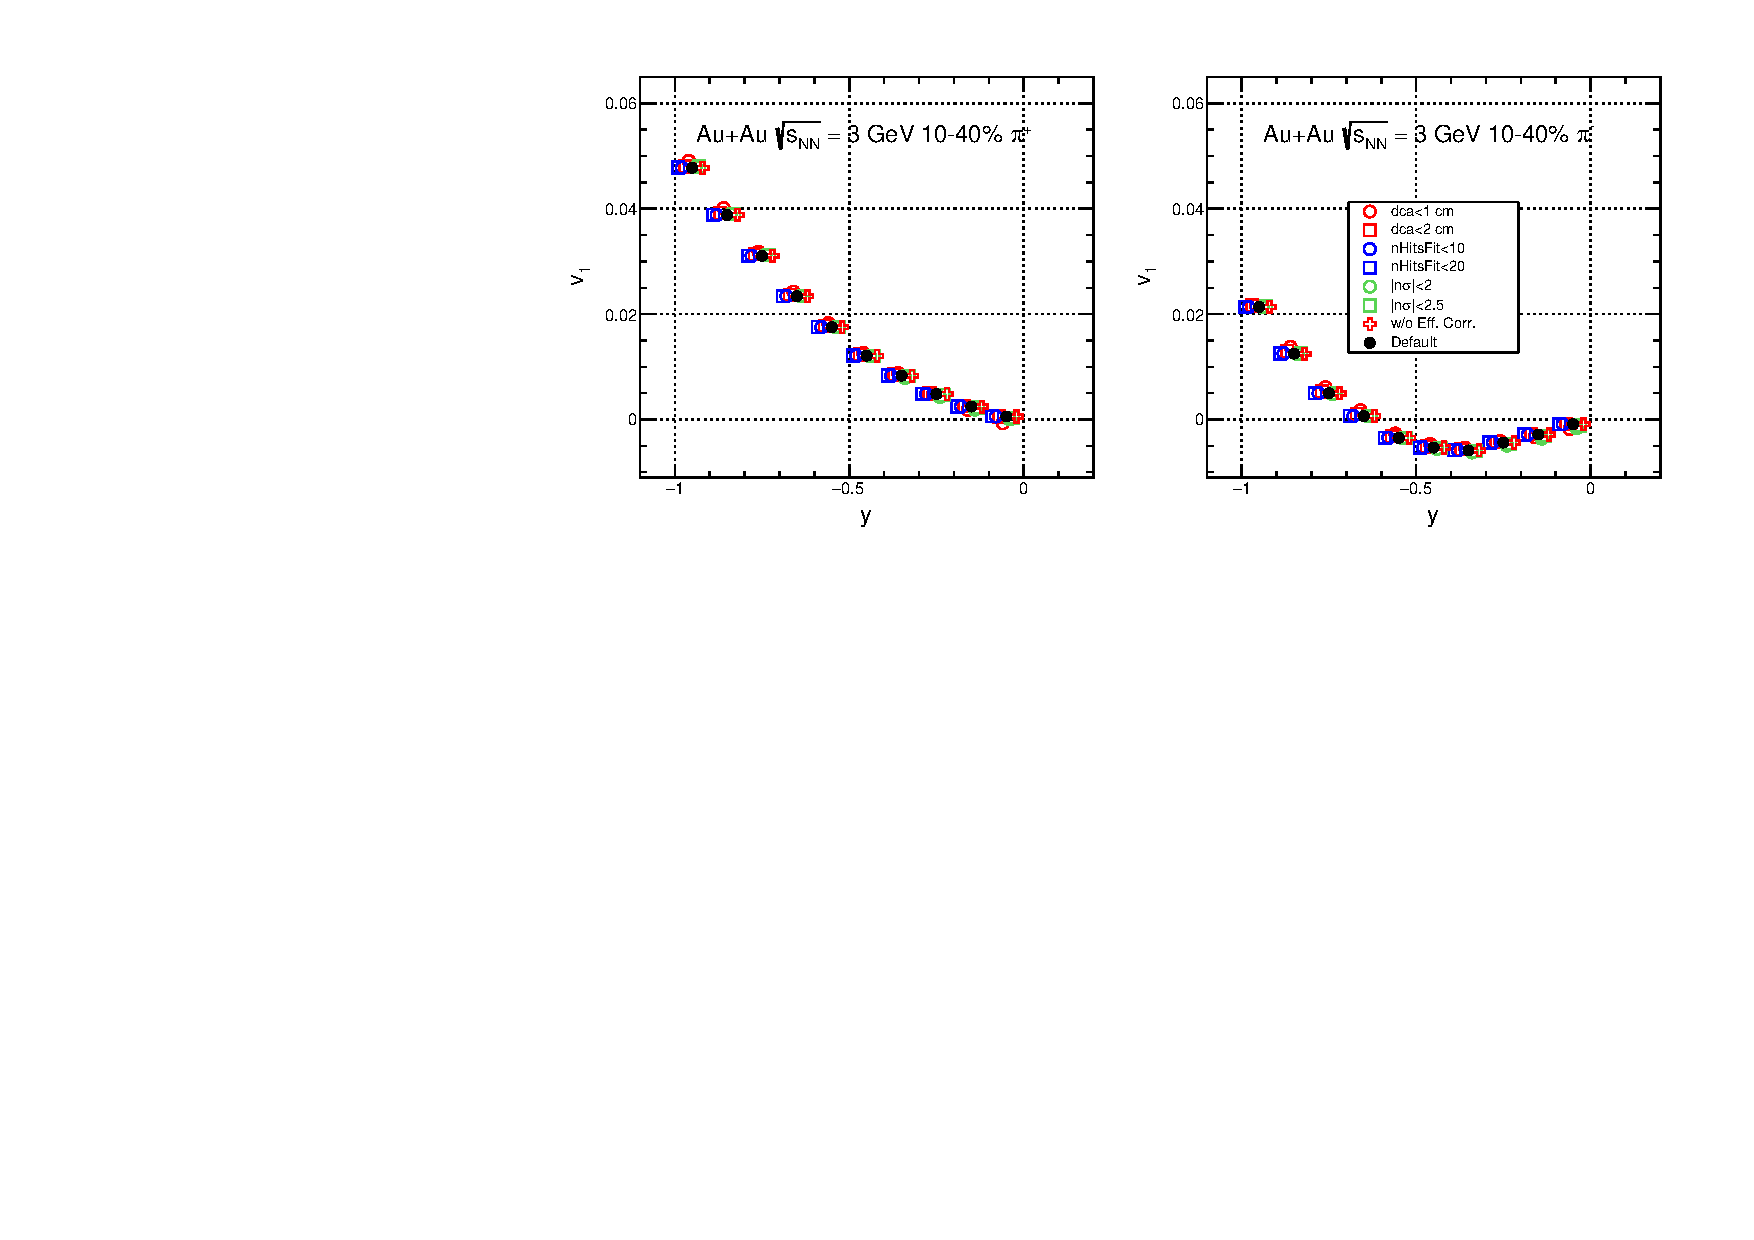
\includegraphics[scale=0.8]{FXT3gev/chapter3/fig/sys/pion/v1y_pion_sys.pdf}
\caption{Systematic uncertainty study for $v_{2}$ as a function of rapidity in 10-40\% for pion at $\sqrt{s_{NN}}$ = 3 GeV.}
\label{fig:pion_v1y_sys}
\end{figure}



\begin{figure}[h]
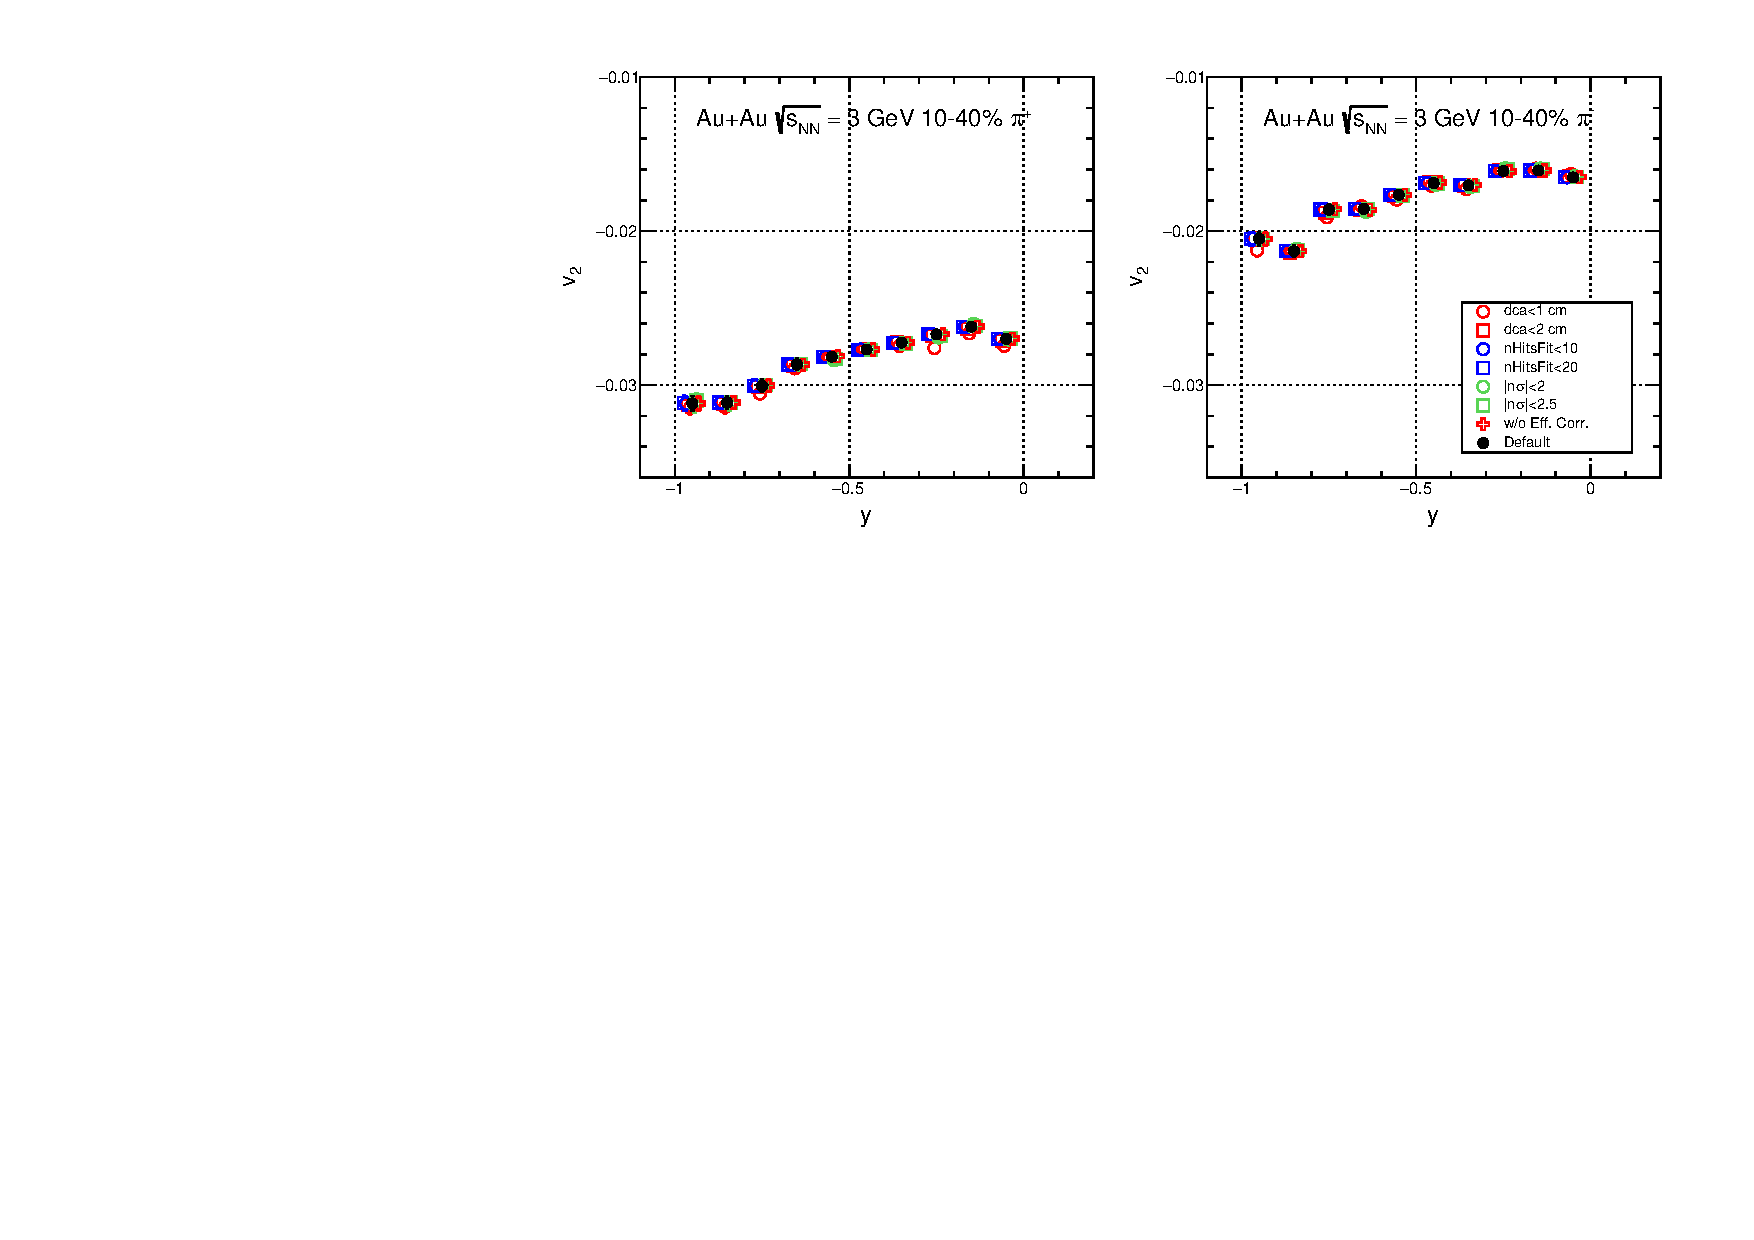
\includegraphics[scale=0.8]{FXT3gev/chapter3/fig/sys/pion/v2y_pion_sys.pdf}
\caption{Systematic uncertainty study for $v_{2}$ as a function of rapidity in 10-40\% for pion at $\sqrt{s_{NN}}$ = 3 GeV.}
\label{fig:pion_v2y_sys}
\end{figure}

\begin{figure}[h]
\includegraphics[scale=0.8]{FXT3gev/chapter3/fig/sys/pion/v1pt_pion_sys.pdf}
\caption{Systematic uncertainty study for $v_{1}$ as a function of $p_{T}$ in 10-40\% for pion at $\sqrt{s_{NN}}$ = 3 GeV}
\label{fig:pion_v1pt_sys}
\end{figure}

\begin{figure}[h]
\includegraphics[scale=0.8]{FXT3gev/chapter3/fig/sys/pion/v2pt_pion_sys.pdf}
\caption{Systematic uncertainty study for $v_{2}$ as a function of $p_{T}$ in 10-40\% for pions at $\sqrt{s_{NN}}$ = 3 GeV.}
\label{fig:pion_v2pt_sys}
\end{figure}


\begin{figure}[h]
\includegraphics[scale=0.8]{FXT3gev/chapter3/fig/sys/kaon/v1y_kaon_sys.pdf}
\caption{Systematic uncertainty study for $v_{1}$ as a function of rapidity in 10-40\% for kaons at $\sqrt{s_{NN}}$ = 3 GeV.}
\label{fig:kaon_v1y_sys}
\end{figure}

\begin{figure}[h]
\includegraphics[scale=0.8]{FXT3gev/chapter3/fig/sys/kaon/v2y_kaon_sys.pdf}
\caption{Systematic uncertainty study for $v_{2}$ as a function of rapidity in 10-40\% for kaons at $\sqrt{s_{NN}}$ = 3 GeV.}
\label{fig:kaon_v2y_sys}
\end{figure}

\begin{figure}[h]
\includegraphics[scale=0.8]{FXT3gev/chapter3/fig/sys/kaon/v1pt_kaon_sys.pdf}
\caption{Systematic uncertainty study for $v_{1}$ as a function of $p_{T}$ in 10-40\% for kaons at $\sqrt{s_{NN}}$ = 3 GeV.}
\label{fig:kaon_v1pt_sys}
\end{figure}

\begin{figure}[h]
\includegraphics[scale=0.8]{FXT3gev/chapter3/fig/sys/kaon/v2pt_kaon_sys.pdf}
\caption{Systematic uncertainty study for $v_{2}$ as a function of $p_{T}$ in 10-40\% for kaons at $\sqrt{s_{NN}}$ = 3 GeV.}
\label{fig:kaon_v2pt_sys}
\end{figure}



\begin{figure}[h]
\includegraphics[scale=0.5]{FXT3gev/chapter3/fig/sys/proton/v1y_proton_sys.pdf}
\caption{Systematic uncertainty study for $v_{1}$ as a function of rapidity in 10-40\% for proton at $\sqrt{s_{NN}}$ = 3 GeV. }
\label{fig:proton_v1y_sys}
\end{figure}

\begin{figure}[h]
\includegraphics[scale=0.5]{FXT3gev/chapter3/fig/sys/proton/v2y_proton_sys.pdf}
\caption{Systematic uncertainty study for $v_{2}$ as a function of rapidity in 10-40\% for proton at $\sqrt{s_{NN}}$ = 3 GeV. }
\label{fig:proton_v2y_sys}
\end{figure}

\begin{figure}[h]
\includegraphics[scale=0.5]{FXT3gev/chapter3/fig/sys/proton/v1pt_proton_sys.pdf}
\caption{Systematic uncertainty study for $v_{1}$ as a function of $p_{T}$ in 10-40\% for proton at $\sqrt{s_{NN}}$ = 3 GeV. }
\label{fig:proton_v1pt_sys}
\end{figure}

\begin{figure}[h]
\includegraphics[scale=0.5]{FXT3gev/chapter3/fig/sys/proton/v2pt_proton_sys.pdf}
\caption{Systematic uncertainty study for $v_{2}$ as a function of $p_{T}$ in 10-40\% for proton at $\sqrt{s_{NN}}$ = 3 GeV. }
\label{fig:proton_v2pt_sys}
\end{figure}


















